%template voor een afstudeerwerk in LaTeX
\documentclass[dutch,11pt,cite,titlepage,oneside]{book}
%''dutch'' voor splitsing en (in emacs) spellingscontrole
\usepackage{babel}   %voor het geval we ook engels nodig hebben
\usepackage{graphicx} %pakket voor includeren figuren
\usepackage{epsfig}
\usepackage[small]{caption}
\usepackage{url}
\usepackage{subfigure}
\usepackage{array}
\usepackage{algorithmic}
\usepackage{multicol}
\usepackage{afterpage}

\usepackage{scriptie}


% lijst met woorden die LaTeX verkeerd splitst
\hyphenation{vaag-ver-za-me-ling L-vaag-ver-za-me-ling} 

\makeindex

\begin{document}

\selectlanguage{dutch}


\newcommand{\auteur}{Klaas Bosteels}
\newcommand{\jaar}{2005--2006}
\newcommand{\titel}{Similariteitsgebaseerd rangschikken van beelden in zoekmachines}
\newcommand{\begeleider}{drs.\ V.\ De Witte en S.\ Schulte}
\newcommand{\richting}{licentiaat in de informatica, optie: software-ontwikkeling}

%de volgende lijn kiest de juiste naam van de vakgroepvoorzitter en de promotor
\newcommand{\vakgroep}{Toegepaste Wiskunde en Informatica}
\newcommand{\voorzitter}{prof.\ dr.\ Guido\ Vanden\ Berghe}
\newcommand{\promotor}{prof.\ dr.\ E.\ E.\ Kerre}


%het titelblad vergt hier en daar enkele manuele ingrepen i.v.m.
%spatiering en dergelijke
\begin{titlepage}
\renewcommand{\baselinestretch}{1.1}
\Large
\begin{center}
\mbox{}\\[0cm]%de volgende lijnen genereren het tempeltje
\unitlength 1mm

\epsfysize 4cm \epsfclipon\epsffile{ruglogo.eps}\\
%\begin{picture}(0,20)
%\centering
%\put(0,11){\makebox(0,0)[b]{\font\aula=aula34 {\aula a}}}
%\put(0,6){\makebox(0,0)[b]{\font\futura=futura scaled 1100
%                 {\futura UNIVERSITEIT}}}
%\put(0,2){\makebox(0,0)[b]{\font\futura=futura scaled 1100
%                 {\futura GENT}}}
%\put(0,0){\makebox(0,0)[b]{\rule{21mm}{1pt}}}
%\end{picture}\\
{\Large 
Faculteit \faculteit\\
Vakgroep \vakgroep\\
Voorzitter: \voorzitter
}\\\vfill
\parbox{14 cm}{
{\Huge\bfseries
\begin{center}
\sf\titel
\end{center}
}
}\\\vfill
door\\ 
{\LARGE \auteur}\\[3.3cm]
%we schrijven ``.\"  i.p.v. ``.'' zodat LaTeX weet dat dit een
%afkorting is (gevolgd door kleine spatie) en niet het einde van een
%zin (gevolgd door lange spatie)
%opmerking: ofwel: prof.\ dr.\ I.\ Lemahieu 
%opmerking: ofwel: prof.\ dr.\ ir.\ W.\ Philips
Promotor: \promotor \\
%Co-promotor: \copromotor \\
Scriptiebegeleiders: \begeleider 
\\\vfill
%        In samenwerking met BARCO GRAPHICS\\
Afstudeerwerk ingediend tot het behalen van de graad van\\
%dit moet uiteraard worden aangepast!
\richting\\[1cm]
Academiejaar \jaar
\end{center}
\renewcommand{\baselinestretch}{1}
\end{titlepage}





%%% Local Variables: 
%%% mode: latex
%%% TeX-master: "total"
%%% End: 
 % de titelpagina


\frontmatter

%\pagenumbering{roman}
%\setcounter{page}{1}

\newpage
\thispagestyle{plain}

\section*{Dankwoord}
Graag zou ik iedereen willen bedanken die heeft bijgedragen tot de
verwezenlijking van dit eindwerk. In het bijzonder dank ik:
\begin{itemize}
  \item mijn promotor \promotor\ en mijn begeleiders \begeleider\ voor het scheppen van de
mogelijkheid dit onderzoek te verrichten
  \item \ldots
\end{itemize}
\vfill

%\newpage
%\thispagestyle{plain}
%\vfill

\section*{Toelating tot bruikleen}
De auteur geeft de toelating dit afstudeerwerk voor consultatie 
beschikbaar te stellen en delen van het afstudeerwerk te kopi\"eren voor
persoonlijk gebruik. Elk ander gebruik valt onder de beperkingen van het 
auteursrecht, in het bijzonder met betrekking tot de verplichting de bron 
uitdrukkelijk te vermelden bij het aanhalen van resultaten uit dit 
afstudeerwerk.
\\[1cm]
\auteur\hfill \today
\\[1cm]             %het voorwoord.
\newpage
\thispagestyle{plain}

\begin{center}
{\sf\huge \titel }\\[3mm]
door\\
{\Large\auteur{}} \\
\end{center}
\noindent Afstudeerwerk ingediend tot het behalen van de graad van
\richting
\vspace{3mm}\\
Academiejaar \jaar
\vspace{3mm}\\
\noindent Universiteit Gent\\
Faculteit Wetenschappen\\
\vspace{3mm}\\
\noindent Promotor: \promotor\\
\noindent Scriptiebegeleiders: \begeleider\\
%\noindent Co-promotor: \copromotor\\
\vfill

%\noindent {\bf\Large Samenvatting}\\[1mm]
\section*{Samenvatting}
De exponenti\"ele groei van het internet geeft aanleiding tot een paradoxale
situatie: hoe meer informatie er beschikbaar komt, hoe moeilijker het wordt
om binnen een redelijke tijd accurate informatie te vinden. Zoekmachines zijn momenteel
de meest gebruikte online service, met miljoenen zoekopdrachten per dag. Naast het zoeken
in teksten, groeit de aandacht voor zogenaamde multimedia zoeksystemen. 

In het bijzonder maken de internetgebruikers steeds meer gebruik van zoekmachines die toelaten om 
gigantische collecties van afbeeldingen te doorzoeken. Deze zoekmachines zijn echter nagenoeg 
allemaal tekst-gebaseerd. Dit houdt in dat het zoeken enkel steunt op het vergelijken van opgegeven 
trefwoorden met tekstuele annotaties die toegekend worden aan elke afbeelding. Het hoeft geen
betoog dat het voor de gebruiker niet altijd gemakkelijk is om op deze manier een aanvaarbaar 
resultaat te vinden. Bovendien worden deze annotaties grotendeels automatisch gegenereerd, 
waardoor ze vaak weinig relevant zijn.

De hierboven genoemde problemen kunnen opgelost worden door het zoeken te baseren op de inhoud 
van de afbeeldingen. De bestaande inhoud-gebaseerde systemen kunnen echter nog altijd niet 
toegepast worden op afbeeldingencollecties van dergelijke grote omvang. In deze scriptie geven 
we daarom een alternatief voor deze meer geavanceerde zoeksystemen, waarbij de grootte van 
te doorzoeken collectie geen probleem vormt. 

Dit alternatief kan gezien worden als een uitbreiding van de tekst-gebaseerde zoeksystemen.
De zoekactie begint nog steeds met het specifi\"eren van \'e\'en of meerdere trefwoorden, waarop
het systeem antwoord met een lijst van relevante afbeeldingen. We zorgen er nu echter voor
dat de gebruiker een aantal voorbeeld-afbeeldingen kan kiezen uit deze lijst, waarna het
systeem de zoekresultaten rangschikt op een manier die de gelijkenis met de voorbeelden uitbuit.

Voor het modelleren van de graduele gelijkenis tussen afbeeldingen, maken we gebruik van 
vaagsimilariteitsmaten. Daarnaast zullen we ook nog beroep doen op aggregatieoperatoren,
zowel voor het combineren van verschillende similariteitsmaten als voor het ondersteunen van
meerdere voorbeeld-afbeeldingen. 
%\vspace{5mm}

%\noindent {\bf\Large Trefwoorden}\\[1mm]
\section*{Trefwoorden}
content-based image retrieval, vaagverzamelingen, similariteitsmaten, aggregatieoperatoren

              %samenvatting  van de thesis

\tableofcontents %genereert de inhoudstafel
%\listoffigures
%\listoftables
%\clearpage


\mainmatter

\chapter{Inleiding}

Op dit eigenste moment zijn er waarschijnlijk enkele honderden \emph{spiders} actief op internet.
Deze computerprogramma's, die soms ook \emph{robots} of \emph{wanderers} worden genoemd, reizen
het internet rond om bepaalde documenten -- in het bijzonder afbeeldingen -- te localiseren. Deze 
documenten worden ge\"indexeerd in een databank, die dan doorzocht kan worden door een zoekmachine. 

Zoekmachines zoals \emph{Google}\footnote{\url{http://www.google.com}} en 
\emph{Yahoo}\footnote{\url{http://www.yahoo.com}} hebben op die manier reeds databanken
opgebouwd die meer dan een miljard afbeeldingen bevatten. Het wordt bijgevolg steeds belangrijker
om manieren te zoeken om deze gigantische collecties van afbeeldingen op een effeci\"ente wijze
te doorzoeken.


\section{Text-based image retrieval}

Nagenoeg alle bestaande zoekmachines bieden \emph{text-based image retrieval} (TBIR) aan. Hierbij
wordt elke afbeelding voorzien van tekstuele annotaties, zoals bijvoorbeeld de 
bestandsnaam of woorden uit de webpagina waarin de afbeelding gebruikt wordt. Deze annotaties
kunnen dan gebruikt worden voor het indexeren van de afbeeldingen in de databank.


\section{Content-based image retrieval}

Omdat de tekst-gebaseerde aanpak in de praktijk dikwijls tekort schiet, is men op zoek gegaan 
naar manier om het zoeken te baseren op de visuele inhoud van de afbeeldingen. Bij 
\emph{content-based image retrieval} (CBIR) maakt men gebruik van een proces dat 
\emph{(visual) feature extraction} genoemd wordt. Dit proces zet een afbeelding om in een 
\emph{feature vector}. Met behulp van multidimensionale indexering kan men deze kenmerkenvector
dan gebruiken als alternatief voor de tekstuele annotaties bij TBIR.


\section{Similariteitsgebaseerd rangschikken}

Door hun grote complexiteit is het vrijwel onmogelijk om \emph{content-based image retrial systems} 
(CBIRSs) te gebruiken voor het doorzoeken van zeer omvangrijke databanken. 
\chapter{Wiskundige fundamenten}

In dit hoofdstuk introduceren we eerst enkele basisbegrippen uit de vaagverzamelingenleer. 
Daarna volgt een overzicht van de vaagsimilariteitsmaten en aggregatieoperatoren waarvan
we later gebruik zullen maken. We hebben dit deel van deze scriptie bewust zo 
bondig mogelijk gehouden. Voor meer informatie verwijzen
we naar \cite{kerre:vaagmodellen}, \cite{vanderweken:similariteitsmaten} en 
\cite{victor:aggregatieoperatoren}.


\section{Basisbegrippen uit de vaagverzamelingenleer}

\subsection{Posets en tralies}
\label{sectie:posets_en_tralies}

In tegenstelling tot de meeste andere gebieden van de wiskunde, wordt in de theorie der 
vaagverzamelingen het begrip ``orde'' ten volle ge\"exploreerd \cite{kerre:vaagmodellen}. Daarom beginnen we deze 
sectie met het defini\"eren van twee ordestructuren: \emph{partieel geordende verzameling} 
(\emph{poset}) en \emph{tralie}. We maken bovendien van de gelegenheid gebruik om enkele 
belangrijke begrippen in verband met posets te introduceren. 

\begin{definitie}
Een partieel geordende verzameling (poset) is een koppel $(P,\le)$ bestaande uit een niet-ledige
verzameling $P$ en een binaire relatie $\le$ over $P$ die reflexief, antisymmetrisch en 
transitief is:
\begin{itemize}
  \item[(P.1)] $(\forall x \in P)(x \le x)$
  \item[(P.2)] $(\forall (x,y) \in P^2)(x \le y \land y \le x \Rightarrow x = y)$
  \item[(P.3)] $(\forall (x,y,z) \in P^3)(x \le y \land y \le z \Rightarrow x \le z)$
\end{itemize}
De relatie $\le$ wordt een (parti\"ele) orderelatie over $P$ genoemd.
\end{definitie} 
\begin{definitie}
Zij $(P,\le)$ een poset en $A \subseteq P$. Een element $b$ van $P$ is een maximaal element
van $A$ als en slechts als $b \in A$ en $(\forall x \in A)(b \le x \Rightarrow x = b)$. 
\end{definitie}
\begin{definitie}
Zij $(P,\le)$ een poset en $A \subseteq P$. Een element $b$ van $P$ is een minimaal element
van $A$ als en slechts als $b \in A$ en $(\forall x \in A)(x \le b \Rightarrow x = b)$. 
\end{definitie}
\begin{definitie}
Zij $(P,\le)$ een poset en $A \subseteq P$. Een element $b$ van $P$ is een bovengrens voor $A$
als en slechts als $(\forall a \in A)(a \le b)$. Als bovendien geldt $b \in A$, dan noemen
we $b$ het grootste element van $A$. De kleinste bovengrens voor $A$ is het
supremum voor $A$.
\end{definitie}
\begin{definitie}
Zij $(P,\le)$ een poset en $A \subseteq P$. Een element $b$ van $P$ is een ondergrens voor $A$
als en slechts als $(\forall a \in A)(b \le a)$. Als bovendien geldt $b \in A$, dan noemen
we $b$ het kleinste element van $A$. De grootste ondergrens voor $A$ is het
infimum voor $A$.
\end{definitie}
\begin{definitie}
Een poset $(L,\le)$ waarin elk doubleton een supremum en een infimum bezit, noemt men een tralie 
(lattice). Als elke niet-ledige deelverzameling van $L$
een supremum en een infimum bezit, dan is $(L, \le)$ een complete tralie.
\end{definitie}
% ALTERNATIEVE DEFINITIE VAN TRALIE
%% enkele nieuwe commando's die we verder in deze sectie nodig zullen hebben
%\newcommand{\dotand}{\ensuremath{\mathaccent\ldotp\land}}
%\newcommand{\dotor}{\ensuremath{\mathaccent\cdotp\lor}}
%\begin{definitie}
%Een algebra\"ische structuur $(L,\dotor,\dotand)$ bestaande uit een niet-ledige
%verzameling $L$ en twee binaire bewerkingen op $L$ wordt een tralie genoemd als en slechts als
%voor elke $a$, $b$ en $c$ uit $L$ geldt:
%\begin{itemize}
%  \item[(L.1)] $a \dotand a = a$ en $a \dotor a = a$
%  \item[(L.2)] $a \dotand b = b \dotand a$ en $a \dotor b = b \dotor a$
%  \item[(L.3)] $a \dotand (b \dotand c) = (a \dotand b) \dotand c$ en $a \dotor (b \dotor c) = (a \dotor b) \dotor c$
%  \item[(L.4)] $a \dotand (a \dotor b) = a$ en $a \dotor (a \dotand b) = a$
%\end{itemize}
%\end{definitie}

\subsection{Vaagverzamelingen}

Het \emph{universum} is de collectie van alle mogelijke elementen (bijvoorbeeld de
natuurlijke getallen). Een verzameling bevat bepaalde elementen uit dat universum (bijvoorbeeld de 
verzameling van de priemgetallen). 

In het geval van een \emph{scherpe (deel)verzameling} behoort elk 
element uit het universum wel of niet tot de verzameling. Andere mogelijkheden zijn er
niet. Een dergelijke verzameling kan bijgevolg 
gerepresenteerd worden door een \emph{karakteristieke afbeelding}, die elk element uit het 
universum afbeeldt op 0 of 1. Dat getal wordt de \emph{lidmaatschapsgraad} van het element 
in kwestie genoemd. De klasse van scherpe verzamelingen in een universum $X$ stellen we voor door 
$\mathcal{P}(X)$.
\begin{definitie}
Zij $X$ een universum. De karakteristieke afbeelding $\mu_A$ van een scherpe verzameling $A$ in $X$
wordt gedefinieerd als de $X - \{0,1\}$ afbeelding:
\begin{displaymath}
\begin{array}{lllll}
\mu_A: 	& X & \to 		& \{0,1\}	& \\
		& x & \mapsto 	& 1,		& \textrm{ als } x \in A \\
		& x & \mapsto 	& 0,		& \textrm{ als } x \notin A
\end{array}
\end{displaymath}
\end{definitie}

Bij een \emph{vaagverzameling} kunnen alle waarden tussen 0 en 1 als lidmaatschapsgraad 
voorkomen. De ``karakteristieke'' afbeelding is in dat geval dus een $X - [0,1]$ afbeelding:
\begin{definitie}
Zij $X$ een universum. Een vaagverzameling $A$ in $X$ wordt gekarakteriseerd door een $X - [0,1]$
afbeelding  $\mu_A$:
\begin{displaymath}
\begin{array}{lllll}
\mu_A: 	& X & \to 		& [0,1]	& \\
		& x & \mapsto 	& \mu_A(x),		& \forall x \in A
\end{array}
\end{displaymath}
\end{definitie}
\noindent
Een element $x \in X$ behoort dus tot de vaagverzameling $A$ met lidmaatschapsgraad $\mu_A(x)$.
Voor de eenvoud noteren we in het vervolg $\mu_A(x)$ steeds als $A(x)$. We maken
met andere woorden geen onderscheid tussen de vaagverzameling en de 
lidmaatschapsfunctie. Voor de klasse van vaagverzamelingen in een universum $X$ gebruiken we
de notatie $\mathcal{F}(X)$.

De \emph{drager} en de \emph{kern} van een vaagverzameling zijn twee belangrijke begrippen: 
\begin{definitie}
De drager van een vaagverzameling $A$ in $X$ wordt gedefinieerd als:
\begin{displaymath}
supp\ A = \{x \in X \mid A(x) > 0\} 
\end{displaymath}
\end{definitie}
\begin{definitie}
De kern van een vaagverzameling $A$ in $X$ wordt als volgt gedefinieerd:
\begin{displaymath}
ker\ A = \{x \in X \mid A(x) = 1\}
\end{displaymath}
\end{definitie}
\noindent
Ook het begrip \emph{cardinaliteit} speelt vaak een belangrijke rol. De cardinaliteit van een 
eindige scherpe verzameling wordt gegeven door het aantal elementen in die verzameling. 
Dat concept kan uitgebreid worden naar vaagverzamelingen door gebruik te maken van het begrip 
\emph{sigma count}:
\begin{definitie}
De sigma count van een vaagverzameling $A$ met eindige drager in een universum $X$ wordt
gedefinieerd door:
\begin{displaymath}
|A|=\sum_{x \in X} A(x)
\end{displaymath}
\end{definitie}

\subsection{Bewerkingen op vaagverzamelingen}
\label{sectie:bew_op_vaagverz}

We beginnen met het defini\"eren van de begrippen \emph{negator}, \emph{conjunctor} en 
\emph{disjunctor}. Die operatoren zijn uitbreidingen van de klassieke logische operatoren
$\lnot$ (negatie), $\land$ (conjunctie) en $\lor$ (disjunctie).
\begin{definitie}
Een negator $\mathcal{N}$ op $[0,1]$ is een dalende $[0,1] - [0,1]$ afbeelding die voldoet
aan de randvoorwaarden $\mathcal{N}(0)=1$ en $\mathcal{N}(1)=0$. 
\end{definitie}
\begin{definitie}
Een conjunctor $\mathcal{C}$ op $[0,1]$ is een stijgende $[0,1]^2 - [0,1]$ afbeelding die voldoet aan de
randvoorwaarden $\mathcal{C}(0,0)=\mathcal{C}(0,1)=\mathcal{C}(1,0)=0$ en $\mathcal{C}(1,1)=1$. 
Als een conjunctor voldoet aan 
$(\forall a \in [0,1])(\mathcal{C}(1,a)=\mathcal{C}(a,1)=a)$ dan is het een semi-norm.
Een driehoeksnorm (t-norm) is een commutatieve en associatieve semi-norm.
\end{definitie}
\begin{definitie}
Een disjunctor $\mathcal{D}$ op $[0,1]$ is een stijgende $[0,1]^2 - [0,1]$ afbeelding die voldoet
aan de randvoorwaarden $\mathcal{D}(1,0)=\mathcal{D}(0,1)=\mathcal{D}(1,1)=1$ en 
$\mathcal{D}(0,0)=0$. Als een disjunctor voldoet aan 
$(\forall a \in [0,1])(\mathcal{D}(0,a)=\mathcal{D}(a,0)=a)$ dan is het een semi-conorm.
Een driehoeksconorm (t-conorm) is een commutatieve en associatieve semi-conorm.
\end{definitie}

De meest gebruikte negator is de standaardnegator $N_s$. Het minimum $T_M$ en het algebra\"isch 
product $T_P$ zijn veelgebruikte t-normen. Bij de t-conormen zijn het maximum $S_M$ en de
probabilistische som $S_P$ dan weer populaire mogelijkheden. Die operatoren worden als 
volgt gedefinieerd:
%\begin{displaymath}
%\begin{array}{r@{\quad=\quad}l}
\begin{align*}
N_s(x) &= 1 - x \\
T_M(x,y) &= \min \{x,y\} \\
T_P(x,y) &= x \cdot y \\
S_M(x,y) &= \max \{x,y\} \\
S_P(x,y) &= x + y - x \cdot y
\end{align*}
%\end{array}
%\end{displaymath}
voor alle $(x,y)$ in $[0,1]^2$.

We kunnen de bovenstaande operatoren nu gebruiken om de klassieke verzameltechnische bewerkingen 
$co$ (complement), $\cap$ (doorsnede) en $\cup$ (unie) te
veralgemenen tot bewerkingen op vaagverzamelingen.
\begin{definitie}
Het $\mathcal{N}$-complement $co_\mathcal{N} A$ van een vaagverzameling $A$ in $X$ wordt gedefinieerd
door de volgende vaagverzameling in X:
\begin{displaymath}
(co_\mathcal{N} A)(x) = \mathcal{N}(A(x)),
\end{displaymath}
voor alle $x$ in $X$, met $\mathcal{N}$ een negator.
\end{definitie}
\begin{definitie}
De $\mathcal{C}$-doorsnede $A \cap_\mathcal{C} B$ van twee vaagverzamelingen $A$ en $B$ in $X$
wordt gedefinieerd door de volgende vaagverzameling in $X$:
\begin{displaymath}
(A \cap_\mathcal{C} B)(x) = \mathcal{C}(A(x),B(x)),
\end{displaymath}
voor alle $x$ in $X$, met $\mathcal{C}$ een conjunctor.
\end{definitie}
\begin{definitie}
De $\mathcal{D}$-unie $A \cup_\mathcal{D} B$ van twee vaagverzamelingen $A$ en $B$ in $X$ wordt gedefinieerd door de
volgende vaagverzameling in $X$:
\begin{displaymath}
(A \cup_\mathcal{D} B)(x) = \mathcal{D}(A(x),B(x)),
\end{displaymath}
voor alle $x$ in $X$, met $\mathcal{D}$ een disjunctor.
\end{definitie}

In het vervolg van deze scriptie zullen we steeds 
$(\mathcal{N},\mathcal{C},\mathcal{D})=(N_s,T_M,S_M)$ kiezen. We voeren daarom de volgende
verkorte notaties in:
\begin{align*}
A^c 			&= co_{N_s} A \\
A \cap B 		&= A \cap_{T_M} B \\
A \cup B		&= A \cup_{S_M} B \\
A \setminus B  	&= A \cap B^c \\
A \triangle B 	&= (A \setminus B) \cup (B \setminus A)
\end{align*}
waarbij $A$ en $B$ vaagverzamelingen in een zelfde universum zijn.


\subsection{L-vaagverzamelingen}

Het begrip vaagverzameling kan op zijn beurt nog eens uitgebreid worden tot 
\emph{L-vaagverzameling}. Die uitbreiding is gebaseerd op het concept \emph{tralie}
uit sectie~\ref{sectie:posets_en_tralies}.
\begin{definitie}
Zij $X$ een universum en $(L,\le)$ een complete tralie. Een L-vaagverzameling $A$ in $X$ wordt
gekarakteriseerd door een $X - L$ afbeelding $\mu_A$:
\begin{displaymath}
\begin{array}{lllll}
\mu_A: 	& X & \to 		& L	& \\
		& x & \mapsto 	& \mu_A(x),		& \forall x \in A
\end{array}
\end{displaymath}
\end{definitie}
\noindent
De klasse van L-vaagverzamelingen in een universum $X$ stellen we voor door 
$\mathcal{F}_L(X)$. Merk op dat die klasse zich herleidt tot $\mathcal{F}(X)$ voor $L = [0,1]$.

\subsection{Bewerkingen op L-vaagverzamelingen}

De begrippen \emph{negator}, \emph{conjunctor} en 
\emph{disjunctor} kunnen uitgebreid worden naar L-vaag\-ver\-za\-me\-ling\-en. Dat heeft als 
gevolg dat de veralgemeende verzameltechnische bewerkingen $co$, $\cap$ en 
$\cup$ uit \ref{sectie:bew_op_vaagverz} eveneens toepasbaar zijn op L-vaagverzamelingen.
We geven hieronder de definities van die uitbreidingen.
Hierbij is $(L,\le)$ een complete tralie die $l$ als kleinste en $u$ als grootste element heeft.
\begin{definitie}
Een negator $\mathcal{N}$ op $L$ is een dalende $L - L$ afbeelding die voldoet
aan de randvoorwaarden $\mathcal{N}(l)=u$ en $\mathcal{N}(u)=l$. 
\end{definitie}
\begin{definitie}
Een conjunctor $\mathcal{C}$ op $L$ is een stijgende $L^2 - L$ afbeelding die voldoet aan de
randvoorwaarden $\mathcal{C}(l,l)=\mathcal{C}(l,u)=\mathcal{C}(u,l)=l$ en $\mathcal{C}(u,u)=u$. 
Als een conjunctor voldoet aan 
$(\forall a \in L)(\mathcal{C}(u,a)=\mathcal{C}(a,u)=a)$ dan is het een semi-norm.
Een driehoeksnorm (t-norm) is een commutatieve en associatieve semi-norm.
\end{definitie}
\begin{definitie}
Een disjunctor $\mathcal{D}$ op $L$ is een stijgende $L^2 - L$ afbeelding die voldoet
aan de randvoorwaarden $\mathcal{D}(u,l)=\mathcal{D}(l,u)=\mathcal{D}(u,u)=u$ en 
$\mathcal{D}(l,l)=l$. Als een disjunctor voldoet aan 
$(\forall a \in L)(\mathcal{D}(l,a)=\mathcal{D}(a,l)=a)$ dan is het een semi-conorm.
Een driehoeksconorm (t-conorm) is een commutatieve en associatieve semi-conorm.
\end{definitie}

\section{Vaagsimilariteitsmaten}
\label{sectie:vaagsimilariteitsmaten}

Het nagaan van de graduele gelijkenis tussen twee vaagverzamelingen -- of tussen twee objecten die 
identificeerbaar zijn met vaagverzamelingen -- kan aan de hand van \emph{vaagsimilariteitsmaten}. 
Een dergelijke similariteitsmaat voor het vergelijken van twee vaagverzamelingen in een 
universum $X$, is niets meer dan een vaagverzameling in $\mathcal{F}(X) \times \mathcal{F}(X)$. De 
lidmaatschapsgraad van een koppel $(A,B) \in (\mathcal{F}(X))^2$ nadert daarbij naar 1 naarmate 
de similariteit tussen de vaagverzamelingen $A$ en $B$ toeneemt.

In \cite{vanderweken:similariteitsmaten} worden er 32 vaagsimilariteitsmaten voorgesteld: $M_1$, $M_2$,
$M_3$, $M_4$, $M_5$, $M_{5c}$, $M_6$, $M_{6c}$, $M_7$, $M_{7c}$, $M_8$, $M_{8c}$, $M_9$, $M_{9c}$,
$M_{10}$, $M_{10c}$, $M_{11}$, $M_{11c}$, $M_{12}$, $M_{13}$, $M_{14a}$, $M_{14b}$, $M_{14c}$, 
$M_{16e}$, $M_{16h}$, $M_{17a}$, $M_{17b}$, $M_{I_3}$, $M_{I_{3c}}$, $M_{18c}$, $M_{20}$ en $M_{20c}$.
We gaan die echter niet allemaal gebruiken. Vooreerst beperken we ons voor
$$
M_1(A,B) = 1 - \left(\frac{1}{|X|} \sum_{x \in X} | A(x) - B(x)|^r\right)^\frac{1}{r} \textrm{ met } 
r \in \{1,2,3,\ldots\}
$$ tot de keuzes
$r=1,2,4$. De overeenkomstige similariteitsmaten noemen we $M_{1a}$, $M_{1b}$ en $M_{1c}$. Vermits
$M_{1a}=M_{18c}$ hoeven we $M_{18c}$ dan niet meer te beschouwen. 
Bovendien zullen we ons enkel
toespitsen op de maten die rechtstreeks uitbreidbaar zijn naar L-vaagverzamelingen met $L=[0,1]^3$. 
Dit houdt in dat we enkel de maten beschouwen die op evidente wijze kunnen veralgemeend worden naar
vaagverzamelingen in $\mathcal{F}_L(X) \times \mathcal{F}_L(X)$. De details van die
uitbreiding behandelen we in \ref{sectie:pixelgeb_kleurbeelden}. 

Zo komen we uiteindelijk tot
de similariteitsmaten die worden weergegeven in tabel~\ref{tab:similatiteitsmaten}. 
Alle vaagsimilariteitsmaten uit die tabel zijn reflexief en symmetrisch. Dat wil zeggen dat 
voor elke maat $M$ geldt: $M(A,A)=1$ en $M(A,B)=M(B,A)$. 

\begin{table}[tbp]
\begin{center}
\begin{tabular}{|l|}
\hline
\\[1pt]
$
\begin{array}{r@{\ }c@{\ }l}
\displaystyle M_{1a}(A,B) & = & \displaystyle 1-\frac{1}{|X|}\sum_{x \in X} | A(x) - B(x) | \\
\displaystyle M_{1b}(A,B) & = & \displaystyle 1-\left(\frac{1}{|X|}\sum_{x \in X} | A(x) - B(x) |^2\right)^\frac{1}{2} \\
\displaystyle M_{1c}(A,B) & = & \displaystyle 1-\left(\frac{1}{|X|}\sum_{x \in X} | A(x) - B(x) |^4\right)^\frac{1}{4} \\
\end{array}
\begin{array}{r@{\ }c@{\ }l}
\displaystyle M_2(A,B) & = & \displaystyle 1 - \max_{x \in X} | A(x) - B(x) | \\[10pt]
\displaystyle M_3(A,B) & = & \displaystyle 1 - \frac{\displaystyle \sum_{x \in X} | A(x) - B(x) |}{\displaystyle |A| + |B|} \\
\end{array}
$
\\
\\[1pt]
\hline
\\[1pt]
$
\begin{array}{r@{\ }c@{\ }l}
\displaystyle M_5(A,B) & = & \displaystyle \frac{\min \{|A|,|B|\}}{\max \{|A|,|B|\}} \\[10pt]
\displaystyle M_{5c}(A,B) & = & \displaystyle \frac{\min \{|A^c|,|B^c|\}}{\max \{|A^c|,|B^c|\}} \\[10pt]
\displaystyle M_6(A,B) & = & \displaystyle \frac{|A \cap B|}{|A \cup B|} \\[10pt]
\displaystyle M_{6c}(A,B) & = & \displaystyle \frac{|A^c \cap B^c|}{|A^c \cup B^c|} \\[10pt]
\displaystyle M_7(A,B) & = & \displaystyle \frac{|A \cap B|}{\max \{|A|,|B|\}} \\[10pt]
\displaystyle M_{7c}(A,B) & = & \displaystyle \frac{|A^c \cap B^c|}{\max \{|A^c|,|B^c|\}} \\[10pt]
\displaystyle M_8(A,B) & = & \displaystyle \frac{|A \cap B|}{\min \{|A|,|B|\}} \\[10pt]
\displaystyle M_{8c}(A,B) & = & \displaystyle \frac{|A^c \cap B^c|}{\min \{|A^c|,|B^c|\}} \\[10pt]
\end{array}
\begin{array}{@{\qquad}r@{\ }c@{\ }l}
\displaystyle M_9(A,B) & = & \displaystyle \frac{\min \{|A|,|B|\}}{|A \cup B|} \\[10pt]
\displaystyle M_{9c}(A,B) & = & \displaystyle \frac{\min \{|A^c|,|B^c|\}}{|A^c \cup B^c|} \\[10pt]
\displaystyle M_{10}(A,B) & = & \displaystyle \frac{\max \{|A|,|B|\}}{|A \cup B|} \\[10pt]
\displaystyle M_{10c}(A,B) & = & \displaystyle \frac{\max \{|A^c|,|B^c|\}}{|A^c \cup B^c|} \\[10pt]
\displaystyle M_{11}(A,B) & = & \displaystyle \frac{\min \{|A \setminus B|,|B \setminus A|\}}{\max \{|A \setminus B|,|B \setminus A|\}} \\[10pt]
\displaystyle M_{11c}(A,B) & = & \displaystyle \frac{\min \{|(A \setminus B)^c|,|(B \setminus A)^c|\}}{\max \{|(A \setminus B)^c|,|(B \setminus A)^c|\}} \\[10pt]
\displaystyle M_{12}(A,B) & = & \displaystyle \frac{|(A \triangle B)^c|}{\max \{|(A \setminus B)^c|,|(B \setminus A)^c|\}} \\[10pt]
\displaystyle M_{13}(A,B) & = & \displaystyle \frac{|(A \triangle B)^c|}{\min \{|(A \setminus B)^c|,|(B \setminus A)^c|\}}
\end{array}
$
\\
\\[1pt]
\hline
\\[1pt]
$
\begin{array}{r@{\ }c@{\ }l}
\displaystyle M_{I_3}(A,B) & = & \displaystyle \frac{|(A \cap B) \cap (A^c \cap B^c)|}{|(A \cup B) \cap (A^c \cup B^c)|}
\end{array}
\begin{array}{@{\qquad}r@{\ }c@{\ }l}
\displaystyle M_{I_{3c}}(A,B) & = & \displaystyle \frac{|(A^c \cap B^c) \cup (A \cap B)|}{|(A^c \cup B^c) \cup (A \cup B)|}
\end{array}
$
\\
\\[1pt]
\hline
\end{tabular}
\caption{\label{tab:similatiteitsmaten}De vaagsimilariteitsmaten die we gaan gebruiken.}
\end{center}
\end{table}



\section{Aggregatieoperatoren} 
\chapter{Enkele begrippen uit beeldverwerking}

We zullen in het vervolg van deze scriptie ook gebruik maken van enkele
begrippen en technieken uit beeldverwerking. In dit hoofdstuk geven we 
een overzicht van die begrippen en beschrijven we kort de corresponderende 
technieken.

\section{Modellering van kleuren en beelden}

\subsection{kleurmodellen}

Een \emph{kleurmodel} is een abstract mathematisch model dat beschrijft hoe kleuren gerepresenteerd 
kunnen worden als $n$-tallen uit $\mathbb{R}^n$. RGB is het meest gebruikte kleurmodel. In dat model is elke kleur
een gewogen som van drie hoofdkleuren: rood, groen en blauw. De gewichten van die som
worden gebruikt als componenten van het drietal dat de kleur voorstelt. 
%Naast RGB zijn ook
%HSV en L*a*b* populaire kleurmodellen \cite{philips:beeldverwerking}.

De kleuren die op basis van een bepaald model kunnen voorgesteld worden, vormen een \emph{kleurruimte}. 
In het geval van RGB is dat een driedimensionale ruimte. De kleuren in die ruimte zijn afhankelijk
van de manier waarop men ``rood'', ``groen'' en ``blauw'' definieert. Veelgebruikte kleurruimtes 
op basis van het RGB model zijn sRGB en Adobe RGB.
Hoewel het strikt gezien niet correct is, wordt de term ``kleurruimte'' vaak ook voor het
kleurmodel gebruikt. Men heeft het dus dikwijls over \emph{de} RGB kleurruimte, terwijl er eigenlijk meerdere
kleurruimtes bestaan die gebaseerd zijn op RGB. 

Ook in het HSV kleurmodel \cite{tkalcic:colour_spaces} wordt elke kleur voorgesteld 
door een drietal. Men noemt de componenten van zo'n drietal respectievelijk 
``hue'', ``saturation'' en ``value''. De eerste van die componenten 
correspondeert met de kleurtint, terwijl de overige componenten de verzadiging 
en de helderheid aangeven. Men kan een kleur $(r,g,b) \in [0,1]^3$ uit het RGB 
model als volgt omzetten naar een kleur $(h,s,v) \in [0,1]^3$ in het HSV model: 
$$
\begin{array}{rcll}
h' & = & 60 \cdot \frac{g - b}{\max \{r,g,b\} - \min \{r,g,b\}}\quad & \textrm{ 
als } \max \{r,g,b\} = r \\[2pt] & = & 60 \cdot \frac{b - r}{\max \{r,g,b\} - 
\min \{r,g,b\}} + 120\quad & \textrm{ als } \max \{r,g,b\} = g \\[2pt] & = & 60 
\cdot \frac{r - g}{\max \{r,g,b\} - \min \{r,g,b\}} + 240\quad & \textrm{ als } 
\max \{r,g,b\} = b \\[6pt] h & = & \frac{h' \bmod 360}{360} & \textrm{ als } h' 
\bmod 360 \geq 0 \\[2pt] & = & \frac{360 - (h' \bmod 360)}{360} & \textrm{ als 
} h' \bmod 360 < 0 \\[6pt] s & = & \frac{\max \{r,g,b\} - \min \{r,g,b\}}{\max 
\{r,g,b\}} & \\[6pt] v & = & \max \{r,g,b\}
\end{array}
$$ Als $s=0$ dan is $h$ niet gedefinieerd. Dat is logisch vermits we dan te 
maken hebben met een grijswaarde. Indien $v=0$ dan is $s$ niet gedefinieerd. We 
hebben het in dat geval dan ook over puur zwart, waarvoor er geen kleurtint of 
verzadiging kan gespecifieerd worden. In de praktische implementatie geven we 
niet gedefinieerde componenten de waarde $0$.

Een kleur in het Irb-model bestaat uit de volgende drie componenten 
\cite{ohta:color_info_for_region_segm}: $$ i = \frac{r+g+b}{3} \qquad r' = 
\frac{r}{r+g+b} \qquad b' = \frac{b}{r+g+b} $$ Hierbij zijn $r,g,b \in [0,1]$ 
de co\"ordinaten van de beschouwde kleur in het RGB-model. 

Het I1I2I3-model, dat werd voorgesteld door Ohta 
\cite{ohta:color_info_for_region_segm}, is een \emph{opponent color space}. 
We zetten een kleur $(r,g,b) \in 
[0,1]^3$ uit het RGB-model als volgt om: $$
%\begin{array}{rcl}
i_1 = \frac{r+g+b}{3} \qquad i_2 = \frac{r-b}{2} \qquad i_3 = \frac{2 \cdot g - 
r - b}{4}
%\end{array}
$$ De eerste component is achromatisch (\emph{white-black}), terwijl de overige 
twee chromatisch zijn (\emph{red-green} en \emph{yellow-blue}).
We gebruiken hier, zoals in \cite{wang:cbir_using_daubechies_wavelets}, een 
genormaliseerde vorm van dit model: $$
%\begin{array}{rcl}
c_1 = \frac{r+g+b}{3} \qquad c_2 = \frac{r + (1 - b)}{2} \qquad c_3 = \frac{r + 
2 \cdot (1 - g) + b}{4}
%\end{array}
$$ 

In het XYZ-model wordt een kleur voorgesteld door de volgende drie componenten: 
$$
\begin{array}{rcl}
x & = & 0.431 \cdot r+0.342 \cdot g+0.178 \cdot b \\ y & = & 0.222 \cdot 
r+0.707 \cdot g+0.071 \cdot b \\ z & = & 0.020 \cdot r+0.130 \cdot g+0.939 
\cdot b
\end{array}
$$ met $(r,g,b) \in [0,1]^3$ de vector van de kleur in het RGB-model. Hierbij 
is $y$ evenredig met de luminantie van de kleur in kwestie. 

De eerste component van een kleur in het Yxy-model is gelijk aan de $y$ 
component van die kleur in het XYZ-model. De overige twee componenten berekenen 
we als volgt: $$ x' = \frac{x}{x+y+z} \qquad y' = \frac{y}{x+y+z} $$ 

Een kleurruimte op basis van het L*a*b*-model is \emph{perceptueel uniform} 
\cite{sharma:digital_color_imaging}. Dat wil zeggen dat, in een dergelijke 
ruimte, de Euclidische afstand een goede maat is voor het waargenomen verschil 
tussen twee kleuren. De co\"ordinaten $(l,a,b)$ van een kleur in het 
L*a*b*-model kunnen als volgt benaderd worden 
\cite{debaets:similariteitsmaten_voor_kleurbeelden, philips:beeldverwerking}: $$
\begin{array}{rcl}
l & = & 116 \cdot f(\frac{100 \cdot y}{y_0}) - 16 \\[5pt] a & = & 500 \cdot 
\left(f(\frac{100 \cdot x}{x_0}) - f(\frac{100 \cdot y}{y_0})\right) \\[5pt] b & = & 200 \cdot 
\left(f(\frac{100 \cdot y}{y_0}) - f(\frac{100 \cdot z}{z_0})\right)
\end{array}
$$ met $$
\begin{array}{rcll}
f(t) & = & t^\frac{1}{3} & \textrm{als } t > 0.008856 \\ & = & 7.787 \cdot t + 
\frac{16}{116} & \textrm{anders}
\end{array}
$$ voor elke re\"ele $t$. Hierbij zijn $x_0$, $y_0$ en $z_0$ de 
XYZ-co\"ordinaten van een wit referentiepunt. We gebruiken hier 
$(x_0,y_0,z_0)=(95.05,100,108.9)$.
We kunnen dan als volgt normaliseren: $$ l' = \frac{l}{100} \qquad a' = \frac{120 + 
\max\{\min\{a,120\},-120\}}{240} \qquad b' = \frac{120 + \max\{\min\{b,120\},-120\}}{240} $$


\subsection{Kleurbeelden}

In een \emph{kleurbeeld} heeft elk beeldpunt een bepaalde kleur, die beschreven wordt met
behulp van een kleurmodel. Met andere woorden: de kleur van een beeldpunt wordt voorgesteld 
als een $n$-tal uit
$\mathbb{R}^n$. Zoals hierboven reeds een aantal keer werd ge\"illustreerd, kunnen dergelijke 
$n$-tallen genormaliseerd worden tot $n$-tallen uit $[0,1]^n$. We kunnen een $m$-dimensionaal 
kleurbeeld dus modelleren als een $\mathbb{R}^m - [0,1]^n$ afbeelding $b$. 
In de praktijk wordt een beeld echter voorgesteld als een rooster bestaande uit een
eindig aantal beeldpunten. Bijgevolg zal $b$ eerder een afbeelding van een deelverzameling van $\mathbb{N}^2$
naar $[0,1]^n$ zijn.

\section{Kleurkwantisatie}
\label{sectie:kleurkwantisatie}

Een kleurruimte bevat meestal een groot aantal 
kleuren. Zo gebruikt men voor een RGB-ruimte bijvoorbeeld typisch 8 bits per 
kleurcomponent. Dit geeft een totaal van 24 bits per kleur, zodat men dus 
$2^{24}=2^4 \cdot 2^{20}=16 \cdot 2^{20} \approx 16 \cdot 10^6$ kleuren kan 
voorstellen.

Om de complexiteit te beperken, kan het dus nodig zijn om het aantal kleuren te 
reduceren. Dat kan door middel van \emph{kleurkwantisatie}. Daarbij groeperen we de kleuren in 
zogenaamde \emph{bins}. We beschouwen dus geen aparte kleuren meer, maar wel 
verzamelingen van kleuren. De kleuren die in dezelfde bin zitten, worden dan 
vervangen door \'e\'en enkele kleur. Het \emph{kleurenpalet} is de verzameling 
van alle bin-kleuren. Bij eenvoudige kwantisatietechnieken wordt steeds 
hetzelfde palet gebruikt, onafhankelijk van de voor te stellen beelden. Meer 
geavanceerde technieken proberen een palet te gebruiken dat optimaal is voor de 
beschouwde beelden.

Wiskundig kunnen we kleurkwantisatie modelleren aan de hand van twee functies: 
$bin$ en $kleur$. De eerste functie associeert met elke kleur $c$, uit de 
kleurruimte $C$, het nummer van de corresponderende bin. Met behulp van de 
tweede functie kan men dan de kleur van die bin bepalen.

\subsection{Uniforme kwantisatie}

Bij \emph{uniforme kwantisatie} wordt elke kleurcomponent uniform verdeeld in een 
aantal intervallen. Als we zorgen dat $C=[0,1]^m$, $m > 0$, dan kunnen we de 
volgende definitie voor $bin$ gebruiken: $$
\begin{array}{lrcll}
bin: & C & \to & \{1,2,...,N\}\\[5pt] & (c_1,c_2,\ldots,c_m) & \mapsto & \left[ 
\sum_{i=1}^m \left( \prod_{j=1}^{i-1} N_j \right) \mathit{fl}(c_i, N_i) \right] 
+ 1, & \forall (c_1,c_2,\ldots,c_m) \in C
\end{array}
$$ met $N_j$ het aantal bins voor de $j$-de component, $N$ het totale aantal 
bins ($N=N_1 \cdot N_2 \cdot \ldots \cdot N_m$) en $$
\begin{array}{rcll}
\mathit{fl}(x,n) & = & \lfloor x \cdot n \rfloor & \textrm{als } x < 1 \\ & = & 
n - 1 & \textrm{als } x = 1
\end{array}
$$ voor alle $x \in [0,1]$ en $n \in \mathbb{N}$. De middelste waarden van de 
intervallen doen hierbij dienst als componenten van de kleur van een bin: $$
\begin{array}{lrcll}
kleur: & \{1,2,\ldots,N\} & \to & C \\ & n & \mapsto & (kleur_1(n), kleur_2(n), 
\dots, kleur_m(n)), & \forall n \in \{1,2,\ldots,N\}
\end{array}
$$ waarbij $$ kleur_i(n) = \frac{n}{\prod_{j=1}^i N_j} + \frac{1}{2 \cdot N_i} 
$$ voor alle $n \in \{1,2,\ldots,N\}$ en $i \in \{1,2,\ldots,m\}$.

Bij image retrieval is doorgaans vooral de kleurtint op zich belangrijk. Door
minder belang te hechten aan de luminantie kan de prestatie zelfs verbeteren,
vermits de similariteitsmaten dan bijvoorbeeld minder afhankelijk zijn van
belichtingsvariaties. Een mogelijke manier om uniform te kwantiseren is dus
het HSV model gebruiken en meer belang hechten aan de eerste kleurcomponent. 
Dat doen we door $N_1=16$, $N_2=4$ en $N_3=4$ te kiezen.
%Bovendien is het discriminerend
%vermogen van dit histogram waarschijnlijk ook beter dan dat van een ongecomprimeerd kleurhistogram.
Die keuzes voor $N_1$, $N_2$ en $N_3$ stemmen overeen met de keuzes die men 
gemaakt heeft voor de \emph{scalable color descriptor} (SCD), die gedefinieerd 
wordt in de MPEG-7 standaard \cite{manjunath:color_and_texture_descriptors}.

Via analoge redeneringen voor de andere kleurmodellen, bekomen we de zes manieren 
uit tabel~\ref{tab:uniforme_kwantisatie} om uniform te kwantiseren met een vast kleurenpalet.
Elk van die manieren gebruikt $256$ bins.

\begin{table}[tbp]
\begin{center}
\begin{tabular}{|c|cccccc|}
\hline
 		& HSV & Irb & I1I2I3 & XYZ & Yxy & L*a*b* \\
\hline
$N_1$ 	& 16 & 4 & 4 & 8 & 4 & 4 \\
$N_2$	& 4  & 8 & 8 & 4 & 8 & 8 \\
$N_3$	& 4  & 8 & 8 & 8 & 8 & 8 \\
\hline
\end{tabular}
\caption{\label{tab:uniforme_kwantisatie}Zes manieren om uniform te kwantiseren met een vast kleurenpalet.}
\end{center}
\end{table}


\subsection{Niet-uniforme kwantisatie}

We hebben reeds vermeld dat bij image retrieval vooral de tinten van de kleuren belangrijk zijn. Daarom 
lijkt het op het eerste zicht geen slecht idee om kleuren met een zelfde kleurtint te groeperen in 
\'e\'en enkele bin. De eerste HSV-component bepaalt dan tot welke bin een kleur behoort. We passen
met andere woorden uniforme HSV-kwantisatie toe met $(N_1,N_2,N_3)=(256,1,1)$. Een probleem daarbij 
is echter dat beelden ook grijswaarden kunnen bevatten. Voor grijswaarden is de ``hue''-component immers 
niet gedefinieerd. De waarde 0 gebruiken voor niet-gedefinieerde kleurtinten lost dit probleem maar 
gedeeltelijk op, want dan komen alle grijswaarden in dezelfde bin terecht. Dat kan wel vermeden worden 
door bijvoorbeeld $(N_1,N_2,N_3)=(64,1,4)$ te kiezen, maar dan kunnen we maar 64 tinten meer onderscheiden.

Met behulp van niet-uniforme kwantisatie komen we tot een betere oplossing. Als we het HSV-model van naderbij
bekijken, dan merken we dat elke kleur getransformeerd kan worden in een grijstint door de verzadiging
voldoende te verlagen. De waarde van de verzadiging waarbij die transformatie plaatsvindt, hangt af
van de helderheid. We gaan daarom als volgt te werk. Als $s > 1 - 0.8 \cdot v$ dan benaderen we de kleur
met de kleurtint en kwantiseren we uniform met $(N_1,N_2,N_3)=(240,1,1)$. In het andere geval hebben we
te maken met een grijstint en kwantiseren we uniform met $(N_1,N_2,N_3)=(1,1,16)$. We combineren dus
twee uniforme kwantisaties tot \'e\'en niet-uniforme. Vermits $240 + 16 = 256$
slagen we er zo in om 240 kleurtinten te onderscheiden, zonder het aantal bins te verhogen. Omdat het
``Perceptually Smooth Color Transition Histogram'' uit \cite{sural:perceptually_smooth_histogram} 
gebaseerd is op deze kwantisatietechniek, spreken we van Smooth Color Transition (SCT) kwantisatie.  

Een andere niet-uniforme manier om te kwantiseren, is het mappen van de kleuren op elf 
\emph{focale kleuren} \cite{van_den_broek:human_color_categorization_for_cbir}: zwart, wit, rood, groen, geen, blauw, bruin, paars, roze, oranje en grijs.
Experimenten hebben aangetoond dat de mens geneigd is om enkel die kleurcategorie\"en te gebruiken bij 
het beredeneren, onthouden en waarnemen van kleuren. We kunnen voor elke kleur de juiste mapping bepalen
door op zoek te gaan naar de focale kleur die in het L*a*b*-model het dichtst bij die gegeven kleur ligt.

\emph{Neural Image Quantization} (NeuQuant) \cite{dekker:neuquant} en de \emph{Wu quantizer} 
\cite{wu:color_quantization_by_dynamic_programming_and_principal_analysis} 
gebruiken, in tegenstelling tot de technieken die we 
tot nu toe bekeken hebben, een variabel kleurenpalet. De eerste techniek is gebaseerd op
Kohonen neurale netwerken, terwijl de tweede gebruik maakt van dynamisch programmeren
en principal analysis. NeuQuant geeft doorgaans iets betere resultaten, maar Wu's techniek is
sneller.

\subsection{Enkele voorbeelden}

\begin{figure}[tbp]
\begin{center}
\subfigure[]{
\includegraphics[height=2.8cm]{images/hsv_constant_s.eps}
\label{fig:hsv_constant_s}
}
\subfigure[]{
\includegraphics[height=2.8cm]{images/hsv_constant_v.eps}
\label{fig:hsv_constant_v}
}
\subfigure[]{
\includegraphics[height=2.8cm]{images/flowers.eps}
\label{fig:flowers}
}
\subfigure[]{
\includegraphics[height=2.8cm]{images/autumn.eps}
\label{fig:autumn}
}
\caption{\label{fig:kwantistatie_originelen}De beelden waarvan we de kleuren gaan kwantiseren op een aantal verschillende manieren.}
\end{center}
\end{figure}

We illustreren de bovenstaande technieken door ze toe te passen op de beelden uit 
figuur~\ref{fig:kwantistatie_originelen}. De eerste twee van die beelden hebben we geconstueerd
door in het HSV-model twee componenten te laten vari\"eren en \'e\'en component constant te houden.
Bij figuur~\ref{fig:hsv_constant_s} is de verzadiging steeds gelijk aan $1$ en laten we de kleurtint 
horizontaal en de helderheid vertikaal vari\"eren. Figuur~\ref{fig:hsv_constant_v} construeren we
op een analoge manier, maar in dit geval is de helderheid constant.

\begin{figure}[tbp]
\begin{center}
\subfigure[]{
\includegraphics[height=2.8cm]{images/uniform_hsv_constant_s.eps}
\includegraphics[height=2.8cm]{images/uniform_hsv_constant_v.eps}
\includegraphics[height=2.8cm]{images/uniform_hsv_flowers.eps}
\includegraphics[height=2.8cm]{images/uniform_hsv_autumn.eps}
\label{fig:uniform_hsv}
}
\subfigure[]{
\includegraphics[height=2.8cm]{images/uniform_irb_constant_s.eps}
\includegraphics[height=2.8cm]{images/uniform_irb_constant_v.eps}
\includegraphics[height=2.8cm]{images/uniform_irb_flowers.eps}
\includegraphics[height=2.8cm]{images/uniform_irb_autumn.eps}
\label{fig:uniform_irb}
}
\subfigure[]{
\includegraphics[height=2.8cm]{images/uniform_i1i2i3_constant_s.eps}
\includegraphics[height=2.8cm]{images/uniform_i1i2i3_constant_v.eps}
\includegraphics[height=2.8cm]{images/uniform_i1i2i3_flowers.eps}
\includegraphics[height=2.8cm]{images/uniform_i1i2i3_autumn.eps}
\label{fig:uniform_i1i2i3}
}
\subfigure[]{
\includegraphics[height=2.8cm]{images/uniform_xyz_constant_s.eps}
\includegraphics[height=2.8cm]{images/uniform_xyz_constant_v.eps}
\includegraphics[height=2.8cm]{images/uniform_xyz_flowers.eps}
\includegraphics[height=2.8cm]{images/uniform_xyz_autumn.eps}
\label{fig:uniform_xyz}
}
\subfigure[]{
\includegraphics[height=2.8cm]{images/uniform_yxy_constant_s.eps}
\includegraphics[height=2.8cm]{images/uniform_yxy_constant_v.eps}
\includegraphics[height=2.8cm]{images/uniform_yxy_flowers.eps}
\includegraphics[height=2.8cm]{images/uniform_yxy_autumn.eps}
\label{fig:uniform_yxy}
}
\subfigure[]{
\includegraphics[height=2.8cm]{images/uniform_lab_constant_s.eps}
\includegraphics[height=2.8cm]{images/uniform_lab_constant_v.eps}
\includegraphics[height=2.8cm]{images/uniform_lab_flowers.eps}
\includegraphics[height=2.8cm]{images/uniform_lab_autumn.eps}
\label{fig:uniform_lab}
}
\caption{\label{fig:kwantistatie_uniform}De resultaten na uniforme kwantisatie op basis van (a) HSV, (b) Irb, (c) I1I2I3, (d) XYZ, (e) Yxy en (f) L*a*b*.}
\end{center}
\end{figure}

Figuur~\ref{fig:kwantistatie_uniform} toont de resultaten die we bekomen door toepassing van de 
zes manieren om uniform te kwantiseren. 

\begin{figure}[tbp]
\begin{center}
\subfigure[]{
\includegraphics[height=2.8cm]{images/sct_constant_s.eps}
\includegraphics[height=2.8cm]{images/sct_constant_v.eps}
\includegraphics[height=2.8cm]{images/sct_flowers.eps}
\includegraphics[height=2.8cm]{images/sct_autumn.eps}
\label{fig:sct}
}
\subfigure[]{
\includegraphics[height=2.8cm]{images/focal_constant_s.eps}
\includegraphics[height=2.8cm]{images/focal_constant_v.eps}
\includegraphics[height=2.8cm]{images/focal_flowers.eps}
\includegraphics[height=2.8cm]{images/focal_autumn.eps}
\label{fig:focal}
}
\subfigure[]{
\includegraphics[height=2.8cm]{images/neuquant_constant_s.eps}
\includegraphics[height=2.8cm]{images/neuquant_constant_v.eps}
\includegraphics[height=2.8cm]{images/neuquant_flowers.eps}
\includegraphics[height=2.8cm]{images/neuquant_autumn.eps}
\label{fig:neuquant}
}
\subfigure[]{
\includegraphics[height=2.8cm]{images/wu_constant_s.eps}
\includegraphics[height=2.8cm]{images/wu_constant_v.eps}
\includegraphics[height=2.8cm]{images/wu_flowers.eps}
\includegraphics[height=2.8cm]{images/wu_autumn.eps}
\label{fig:wu}
}
\caption{\label{fig:kwantistatie_uniform}De resultaten na niet-uniforme kwantisatie op basis van (a) SCT, (b) focale kleuren, (c) NeuQuant en (d) de Wu quantizer.}
\end{center}
\end{figure}

\section{Lineaire filters}

Bij het \emph{filteren} van een 2-dimensionaal beeld $b$ wordt de waarde van elk beeldpunt $(x,y) \in \mathbb{N}^2$ 
vervangen door een nieuwe waarde die afhangt van de originele waarde $b(x,y)$ van het beeldpunt en van de waarden 
van naburige beeldpunten. In het geval van een \emph{lineair filter} is die nieuwe waarde een lineaire combinatie 
van de oude waarden. Het beeld $b'$ dat we bekomen door $b$ lineair te filteren, wordt gegeven door
de volgende correlatie \cite{philips:beeldverwerking}:
$$
b'(x,y) = \sum_{(x',y') \in \Omega_m} b(x+x',y+y')m(x',y')
$$
met $m$ een re\"eelwaardige functie en $\Omega_m = \{ (x,y) \mid m(x,y) \ne 0 \}$. De functie $m$ wordt
het \emph{filtermasker} genoemd.

Het \emph{3x3 binomiaalfilter} is een voorbeeld van een lineair filter. Voor het filtermasker 
$m_{bin}$ van dat filter geldt $m_{bin}(-1,-1)=m_{bin}(-1,1)=m_{bin}(1,-1)=m_{bin}(1,1)=1/16$, 
$m_{bin}(-1,0)=m_{bin}(0,-1)=m_{bin}(1,0)=m_{bin}(0,1)=1/8$, $m_{bin}(0,0)=1/4$ en 
$m_{bin}(x,y)=0$ voor de overige $(x,y)$. Als we veronderstellen dat $m_{bin}(x,y)=0$ voor de 
posities $(x,y)$ die niet weergegeven worden, dan kunnen we dat masker noteren als een matrix:
$$
\frac{1}{16}\left[ \begin{array}{ccc} 1 & 2 & 1\\ 2 & 4 & 2\\ 1 & 2 & 1 \end{array} \right]
= \frac{1}{16}\left[ \begin{array}{c} 1\\ 2\\ 1 \end{array} \right] \cdot 
\left[ \begin{array}{ccc} 1 & 2 & 1 \end{array} \right]
$$
Zoals weergegeven in figuur~\ref{fig:indische_ruizig_en_binom}, kan een binomiaalfilter gebruikt worden om ruis te onderdrukken.

\begin{figure}[tb]
\begin{center}
\subfigure[]{
\includegraphics[width=0.4\textwidth]{images/indische_ruizig.eps}
\label{fig:indische_ruizig}
}
\subfigure[]{
\includegraphics[width=0.4\textwidth]{images/indische_binom.eps}
\label{fig:indische_binom}
}
\caption{\label{fig:indische_ruizig_en_binom}Een ruizig beeld (a) en het resultaat na filteren met een 5x5 binomiaalfilter (b).}
\end{center}
\end{figure}

\section{Eenvoudige randdetectie}

Beeldranden in een 2-dimensionaal beeld $b$ zijn plaatsen waar de luminantiecomponent $l(x,y)$ van $b(x,y)$ 
sterk varieert als functie van $x$ en/of $y$. Op die plaatsen zullen de partieel afgeleiden $D_1 l(x,y)$ en 
$D_2 l(x,y)$ dus groot zijn. Bijgevolg zal de \emph{gradi\"ent} $\nabla l$ daar ook groot zijn. We kunnen 
dus de volgende formule gebruiken om randen te detecteren in $b$: 
$$
|\nabla l(x,y)| = \sqrt{(D_1 l(x,y))^2 + (D_2 l(x,y))^2}
$$ 
met $l$ de $\mathbb{N}^2 - [0,1]$ afbeelding die met elk beeldpunt $(x,y)$ de juiste luminantiecomponent associeert.

Doordat $l$ in de praktijk geen continue maar een discrete functie is, moeten we de partieel afgeleiden benaderen.
De Taylorreeksontwikkeling van een $\mathbb{R} - \mathbb{R}$ functie $f$ rond $x$ geeft
$$
f(x+h) = f(x) + h D f(x) + \frac{h^2}{2!} D^2 f(x) + \ldots
$$
en ook
$$
f(x-h) = f(x) - h D f(x) + \frac{h^2}{2!} D^2 f(x) + \ldots
$$
zodat
$$
\frac{f(x+h) - f(x-h)}{2h} \approx D f(x)
$$
Bijgevolg geldt $D_1 l(x,y) \approx (l(x+1,y) - l(x-1,y))/2$ en $D_2 l(x,y) \approx (l(x,y+1) - l(x,y-1))/2$. We
kunnen de eerste en tweede partieel afgeleiden dus berekenen met behulp van lineaire filters met filtermaskers:
$$
D_1 l(x,y)\textrm{: }\quad \frac{1}{2} \left[ \begin{array}{ccc} -1 & 0 & 1 \end{array} \right] \qquad \textrm{ en } 
\qquad D_2 l(x,y)\textrm{: }\quad \frac{1}{2} \left[ \begin{array}{c} -1 \\ 0 \\ 1 \end{array} \right]
$$
De \emph{Sobel-operator} is een variant hierop die minder ruisgevoelig is doordat er 
extra ruisonderdrukking voorzien wordt via een binomiaalfilter loodrecht op de richting 
van de parti\"ele afleiding:
$$
D_1 l(x,y)\textrm{: }\quad \frac{1}{8} \left[ \begin{array}{c} 1 \\ 2 \\ 1 \end{array} \right] \cdot \left[ \begin{array}{ccc} -1 & 0 & 1 \end{array} \right] \qquad \textrm{ en } 
\qquad D_2 l(x,y)\textrm{: }\quad \frac{1}{8} \left[ \begin{array}{ccc} 1 & 2 & 1 \end{array} \right] \cdot \left[ \begin{array}{c} -1 \\ 0 \\ 1 \end{array} \right]
$$
Uit figuur~\ref{fig:randdetectie} blijkt echter dat beide technieken geen spectaculair verschillende 
resultaten geven.

\begin{figure}[tb]
\begin{center}
\subfigure[]{
\includegraphics[width=0.3\textwidth]{images/lena.eps}
\label{fig:lena}
}
\subfigure[]{
\includegraphics[width=0.3\textwidth]{images/lena_gradient.eps}
\label{fig:lena_gradient}
}
\subfigure[]{
\includegraphics[width=0.3\textwidth]{images/lena_sobel.eps}
\label{fig:lena_sobel}
}
\caption{\label{fig:randdetectie}Het origineel luminantiebeeld (a) en het resultaat na filteren met een gradi\"ent-filter (b) en met een Sobel-filter (c).}
\end{center}
\end{figure}
\chapter{Similariteitsmaten voor beelden}

Een similariteitsmaat voor beelden is een maat die de gelijkenis tussen twee gegeven
beelden uitdrukt als een getal in het eenheidsinterval $[0,1]$. Dat getal nadert naar 1
naarmate de gelijkenis groter is. Bijgevolg kunnen we een dergelijke maat gebruiken om
een lijst van zoekresultaten te herordenen volgens similariteit met een bepaald 
voorbeeld uit die lijst. 

We construeren een similariteitsmaat voor beelden in twee stappen. Eerst identificeren we
een beeld, al dan niet rechtstreeks, met een (L-)vaagverzameling. Daarna maken we gebruik van
de vaagsimilariteitsmaten uit \ref{sectie:vaagsimilariteitsmaten} om die (L-)vaagverzamelingen te
vergelijken. 

In het vervolg van deze scriptie bedoelen we met de term ``similariteitsmaat'' steeds
een similariteitsmaat voor beelden. We gebruiken die term dus niet voor een vaagsimilariteitsmaat
op zich, maar wel voor de combinatie van een dergelijke vaagsimilariteitsmaat met een manier om beelden te 
identificeren met (L-)vaagverzamelingen.

\section{Eigenschappen}

In de volgende hoofdstukken construeren we een aantal similariteitsmaten voor beelden. Daarbij 
eisen we dat al onze similariteitsmaten \defin{reflexief} en \defin{symmetrisch} zijn.

\subsection{Reflexiviteit}

Voor twee identieke beelden verwachten we dat een similariteitsmaat $M$ als resultaat $1$
teruggeeft. Met andere woorden, voor een beeld $A$ moet gelden: $M(A,A)=1$.
Die eigenschap heeft als gevolg dat het voorbeeld zich steeds vooraan in
de geordende lijst van zoekresultaten moet bevinden.

\subsection{Symmetrie}

Het resultaat van een similariteitsmaat $M$ wordt verwacht onafhankelijk te zijn van de 
volgorde waarin de beelden aangeboden worden. Voor beelden $A$ en $B$ moet dus gelden:
$M(A,B)=M(B,A)$.

\subsection{Transitiviteit}

De bovenstaande eigenschappen doen denken aan een klassieke equivalentierelatie. Dergelijke
relaties zijn naast reflexief en symmetrisch ook transitief. In 
\cite{zadeh:similarity_relations_and_fuzzy_orderings} definieert Zadeh
de \defin{similariteitsrelatie} als vage uitbreiding van dat scherpe begrip. Als we zouden
afdwingen dat een similariteitsmaat $M$ een similariteitsrelatie is, dan moet $M$ 
\defin{min-transitief}{$\min$-transitief} zijn: voor drie beelden $A$, $B$ en $C$ moet 
$\min\{M(A,B),M(B,C)\} \le M(A,C)$ gelden. Die
eigenschap komt echter niet overeen met de intu\"itieve betekenis van similariteit
\cite{de_cock:on_unsuitable_relations_for_approx_equal, de_cock:why_fuzzy_relations_do_not_resolve_pointcare_paradox}. 
Beschouw bijvoorbeeld de afzonderlijke beelden $A_i$, $i \in \{1,2,\ldots,n\}$, uit \'e\'en sc\`ene van een video. 
Daarbij zullen opeenvolgende beelden doorgaans zeer similair zijn, met andere woorden: 
$M(A_i,A_{i+1}) \approx 1$ voor $i \in \{1,2,\ldots,n-1\}$. Uit de $\min$-transitiviteit
zou dan volgen dat ook $M(A_1,A_n) \approx 1$, terwijl het eerste en het laatste beeld
van een sc\`ene meestal sterk verschillend zijn.   

\section{Evaluatie van performantie}

\subsection{Globale genormaliseerde gemiddelde rang (GGGR)}

Om uit meerdere similariteitsmaten de meest geschikte te kiezen, 
moeten we een manier vinden om een dergelijke maat objectief te beoordelen. 
Dat doen we door, voor een bepaald voorbeeld, elke maat toe te passen op eenzelfde collectie 
van beelden. Vervolgens beoordelen we de zo bekomen rangschikking met behulp van een performantiemaat.

Figuur~\ref{fig:testcollectie} bevat de collectie van beelden die we gaan 
gebruiken. Die collectie bestaat uit een selectie van beelden uit
de \defin{Columbia object image library} \cite{coil-100}, die gegenereerd werd 
door een aantal roterende objecten op bepaalde vaste momenten te fotograferen. 
Onze testcollectie bestaat uit foto's van elf objecten. Van elk object zijn
er zes momentopnames, wat een totaal van $11 \cdot 6 = 66$ beelden geeft.

\begin{figure}[p]
\vspace{5pt}
\centering

\begin{tabular}{cccccc}

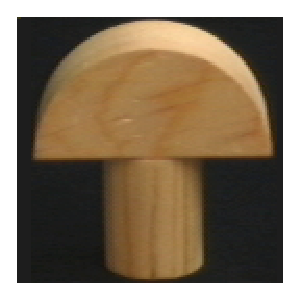
\includegraphics[width=2cm]{coil/beeld-0.eps} &
\includegraphics[width=2cm]{coil/beeld-1.eps} &
\includegraphics[width=2cm]{coil/beeld-2.eps} &
\includegraphics[width=2cm]{coil/beeld-3.eps} &
\includegraphics[width=2cm]{coil/beeld-4.eps} &
\includegraphics[width=2cm]{coil/beeld-5.eps} \\

\includegraphics[width=2cm]{coil/beeld-42.eps} &
\includegraphics[width=2cm]{coil/beeld-43.eps} &
\includegraphics[width=2cm]{coil/beeld-44.eps} &
\includegraphics[width=2cm]{coil/beeld-45.eps} &
\includegraphics[width=2cm]{coil/beeld-46.eps} &
\includegraphics[width=2cm]{coil/beeld-47.eps} \\

\includegraphics[width=2cm]{coil/beeld-12.eps} &
\includegraphics[width=2cm]{coil/beeld-13.eps} &
\includegraphics[width=2cm]{coil/beeld-14.eps} &
\includegraphics[width=2cm]{coil/beeld-15.eps} &
\includegraphics[width=2cm]{coil/beeld-16.eps} &
\includegraphics[width=2cm]{coil/beeld-17.eps} \\

\includegraphics[width=2cm]{coil/beeld-18.eps} &
\includegraphics[width=2cm]{coil/beeld-19.eps} &
\includegraphics[width=2cm]{coil/beeld-20.eps} &
\includegraphics[width=2cm]{coil/beeld-21.eps} &
\includegraphics[width=2cm]{coil/beeld-22.eps} &
\includegraphics[width=2cm]{coil/beeld-23.eps} \\

\includegraphics[width=2cm]{coil/beeld-24.eps} &
\includegraphics[width=2cm]{coil/beeld-25.eps} &
\includegraphics[width=2cm]{coil/beeld-26.eps} &
\includegraphics[width=2cm]{coil/beeld-27.eps} &
\includegraphics[width=2cm]{coil/beeld-28.eps} &
\includegraphics[width=2cm]{coil/beeld-29.eps} \\

\includegraphics[width=2cm]{coil/beeld-54.eps} &
\includegraphics[width=2cm]{coil/beeld-55.eps} &
\includegraphics[width=2cm]{coil/beeld-56.eps} &
\includegraphics[width=2cm]{coil/beeld-57.eps} &
\includegraphics[width=2cm]{coil/beeld-58.eps} &
\includegraphics[width=2cm]{coil/beeld-59.eps} \\

\includegraphics[width=2cm]{coil/beeld-30.eps} &
\includegraphics[width=2cm]{coil/beeld-31.eps} &
\includegraphics[width=2cm]{coil/beeld-32.eps} &
\includegraphics[width=2cm]{coil/beeld-33.eps} &
\includegraphics[width=2cm]{coil/beeld-34.eps} &
\includegraphics[width=2cm]{coil/beeld-35.eps} \\

\includegraphics[width=2cm]{coil/beeld-36.eps} &
\includegraphics[width=2cm]{coil/beeld-37.eps} &
\includegraphics[width=2cm]{coil/beeld-38.eps} &
\includegraphics[width=2cm]{coil/beeld-39.eps} &
\includegraphics[width=2cm]{coil/beeld-40.eps} &
\includegraphics[width=2cm]{coil/beeld-41.eps} \\

\includegraphics[width=2cm]{coil/beeld-6.eps} &
\includegraphics[width=2cm]{coil/beeld-7.eps} &
\includegraphics[width=2cm]{coil/beeld-8.eps} &
\includegraphics[width=2cm]{coil/beeld-9.eps} &
\includegraphics[width=2cm]{coil/beeld-10.eps} &
\includegraphics[width=2cm]{coil/beeld-11.eps} \\

\includegraphics[width=2cm]{coil/beeld-48.eps} &
\includegraphics[width=2cm]{coil/beeld-49.eps} &
\includegraphics[width=2cm]{coil/beeld-50.eps} &
\includegraphics[width=2cm]{coil/beeld-51.eps} &
\includegraphics[width=2cm]{coil/beeld-52.eps} &
\includegraphics[width=2cm]{coil/beeld-53.eps} \\

\includegraphics[width=2cm]{coil/beeld-60.eps} &
\includegraphics[width=2cm]{coil/beeld-61.eps} &
\includegraphics[width=2cm]{coil/beeld-62.eps} &
\includegraphics[width=2cm]{coil/beeld-63.eps} &
\includegraphics[width=2cm]{coil/beeld-64.eps} &
\includegraphics[width=2cm]{coil/beeld-65.eps} \\

\end{tabular}
\vspace{5pt}
\caption{\label{fig:testcollectie}De gebruikte collectie van beelden.}
\end{figure}

Voor het beoordelen van een rangschikking, gebruiken we de \defin{genormaliseerde gemiddelde rang} 
(GGR) \cite{muller:perf_eval}. Die performantiemaat wordt toegepast op een collectie
van $N$ beelden. Voor elk van die beelden bevat de collectie
$N_R$ zogenaamde \defin{relevante beelden}. In het geval van onze testcollectie geldt $N = 66$.
We gaan er in die collectie van uit dat foto's van eenzelfde object relevant zijn ten opzichte
van elkaar: $N_R = 6$. Beschouw nu de vector 
$(r_1,r_2,\ldots,r_{N_R}) \in \{1,2,\ldots,N\}^{N_R}$, waarbij $r_i$ het
rangnummer van het $i$-de relevante beeld voorstelt. De performantiemaat
wordt dan als volgt gedefinieerd:
\begin{definitie}
De genormaliseerde gemiddelde rang wordt gegeven door de volgende afbeelding:
\begin{displaymath}
\begin{array}{lrcl}
\textrm{GGR}: 	& \{1,2,\ldots,N\}^{N_R} & \to 	& [0,1] \\
		& (r_1,r_2,\ldots,r_{N_R}) & \mapsto &
	{\displaystyle\frac{1}{N \cdot N_R}\left[ \left(\sum_{i=1}^{N_R}r_i\right) - \frac{N_R \cdot (N_R + 1)}{2} \right]},\\[15pt]
	& & & \qquad \quad \forall (r_1, r_2, ..., r_{N_R}) \in \{1,2,\ldots,N\}^{N_R}
\end{array}
\end{displaymath}
\end{definitie}
\noindent
Deze maat nadert naar 1 naarmate de performantie slechter wordt.

Tot nu toe hebben we er nog geen rekening mee gehouden dat de performantie van
een similariteitsmaat afhankelijk kan zijn van het gekozen voorbeeld. Dat probleem lossen we
op door de GGR te berekenen voor meerdere voorbeelden en het gemiddelde van de bekomen waarden
te beschouwen. We kiezen daarbij de beelden uit de linker kolom van 
figuur~\ref{fig:testcollectie} als voorbeeld. De waarde die we zo bekomen noemen we de
\defin{genormaliseerde gemiddelde rang!globale}{globale genormaliseerde gemiddelde rang} 
(GGGR). Het is die waarde die we zullen gebruiken
om de performantie van een similariteitsmaat te evalueren. We zullen dus met andere woorden op
zoek gaan naar similariteitsmaten waarvan de GGGR zo klein mogelijk is.

\subsection{Rekentijd}

Voor elke similariteitsmaat die we construeren meten we ook hoe lang het duurt om
de rangschikkingen, die nodig zijn om de GGGR te bepalen, te berekenen. Aan die 
rekentijd hechten we echter niet zoveel belang als aan de GGGR, vermits het in onze
praktische implementatie niet absoluut noodzakelijk is dat de similariteitsmaten zo weinig
mogelijk rekentijd vereisen. De collecties van beelden waarop ze daarbij toegepast worden,
zijn immers beperkt in grootte. Bovendien worden de berekeningen aan de kant van de client
uitgevoerd, waardoor er geen gevaar is voor overbelasting van de server.

Indien we de similariteitsmaten zouden construeren voor een zuiver CBIR-systeem, zoals weergegeven
in figuur~\ref{fig:cbir}, dan zou de rekentijd wel zeer belangrijk zijn. Hoewel het aantal
beelden beperkt wordt door het gebruik van multidimensionale indexering, zal een dergelijk
systeem de similariteitsmaten immers toch nog moeten toepassen op een groot aantal
beelden. Anderzijds laat een zuiver CBIR-systeem wel toe om berekeningen op voorhand te doen
en de resultaten ervan samen met de beelden op te slaan in de databank. Bij het similariteitsgebaseerd
rangschikken van de zoekresultaten is dat niet mogelijk, omdat de databank daarbij niet rechtstreeks
toegankelijk is.

Als we het bepalen van de similariteiten vergelijken met het studeren voor een examen, dan 
heeft de student in het geval van echte CBIR op voorhand meer dan voldoende tijd om de leerstof
te verwerken. Vlak voor het examen is er echter maar net genoeg tijd om alles nog eens 
te herhalen. Bij het similariteitsgebaseerd rangschikken van de zoekresultaten kan er niet vooraf 
gestudeerd worden, maar juist voor het examen heeft de student wel nog enkele dagen ter beschikking 
om alles in te studeren.


\section{Beperken van de rekentijd}
\label{sectie:beperken_rekentijd}

Hoewel de rekentijd voor onze praktische toepassing niet van cruciaal belang is, kan het beperken 
ervan uiteraard geen kwaad. Door toch voldoende aandacht te schenken aan de rekentijd kunnen
we er zelfs voor zorgen dat similariteitsmaten waarvoor we zonder extra inspanning veel te lang zouden 
moeten rekenen, toch nog bruikbaar zijn.

Stel dat $A$ en $B$ twee vaagverzamelingen zijn in een zelfde universum $X$. Het kan dan voorkomen dat 
$X'= supp\ A \cup supp\ B$ veel minder elementen bevat dan $X$. In dat geval kunnen we de rekentijd sterk
reduceren door het bereik van de sommaties in de vaagsimilariteitsmaten te beperken tot $X'$. Doordat
$A(x)=B(x)=0$ voor alle $x \in X \setminus X'$ geldt er dan immers zowel
\begin{align*}
\displaystyle \sum_{x \in X} | A(x) - B(x) | 
&= \displaystyle \sum_{x \in X \setminus X'} | A(x) - B(x) | + \displaystyle \sum_{x \in X'} | A(x) - B(x) | \\
&= \displaystyle \sum_{x \in X \setminus X'} | 0 - 0 | + \displaystyle \sum_{x \in X'} | A(x) - B(x) | \\
&= \displaystyle \sum_{x \in X'} | A(x) - B(x) |
\end{align*}
als $|A| = \sum_{x \in X} A(x) = \sum_{x \in X \setminus X'} 0 + \sum_{x \in X'} A(x) 
= \sum_{x \in X'} A(x)$.
% \begin{displaymath}
% |A| = \sum_{x \in X} A(x) = \sum_{x \in X \setminus X'} A(x) + \sum_{x \in X'} A(x) 
% = \sum_{x \in X \setminus X'} 0 + \sum_{x \in X'} A(x) = \sum_{x \in X'} A(x)
% \end{displaymath}
Wanneer we 
\begin{displaymath}
||A|| = \sum_{x \in X'} A(x)
\end{displaymath} 
defini\"eren, dan geldt dus $|A| = ||A||$ en ook:
\begin{align*}
| A \cap B | 
&= \displaystyle \sum_{x \in X} T_M(A(x),B(x)) & & \\
&= \displaystyle \sum_{x \in X'} T_M(A(x),B(x)) & & (T_M(0,0)=0) \\
&= ||A \cap B|| & & \displaybreak[0] \\ %[5pt]
| A \cup B | 
&= \displaystyle \sum_{x \in X} S_M(A(x),B(x)) & & \\
&= \displaystyle \sum_{x \in X'} S_M(A(x),B(x)) & & (S_M(0,0)=0) \\
&=  ||A \cup B|| & & \displaybreak[0] \\ %[5pt]
| A \setminus B | = | A \cap B^c | 
&= \displaystyle \sum_{x \in X} T_M(A(x),1-B(x)) & & \\
&= \displaystyle \sum_{x \in X'} T_M(A(x),1-B(x)) & & (T_M(0,1-0)=T_M(0,1)=0) \\
&= || A \cap B^c || = ||A \setminus B|| & & %\\[5pt]
\end{align*}
Doordat $T_M(0,1)=0$ en $S_M(0,0)=0$ geldt eveneens
% \begin{align*}
% | A \triangle B | 
% &= | (A \setminus B) \cup (B \setminus A) | & & \\
% &= || (A \setminus B) \cup (B \setminus A) || & & (T_M(0,1)=0 \textrm{ en } S_M(0,0)=0) \\
% &= || A \triangle B || & & \\
% \end{align*}
\begin{displaymath}
| A \triangle B | = | (A \setminus B) \cup (B \setminus A) | = || (A \setminus B) \cup (B \setminus A) || = || A \triangle B ||
\end{displaymath}
% \end{align*}
en uit $T_M(0,1)=0$ volgt dat 
% \begin{align*}
% |(A \cap B) \cap (A^c \cap B^c)| &= ||(A \cap B) \cap (A^c \cap B^c)|| & & (T_M(0,1)=0)\\ %[5pt]
% |(A \cup B) \cap (A^c \cup B^c)| &= ||(A \cup B) \cap (A^c \cup B^c)|| & & (T_M(0,1)=0)
% \end{align*}
$|(A \cap B) \cap (A^c \cap B^c)| = ||(A \cap B) \cap (A^c \cap B^c)||$ en
$|(A \cup B) \cap (A^c \cup B^c)| = ||(A \cup B) \cap (A^c \cup B^c)||$.
Met behulp van de eigenschap
\begin{displaymath}
|A^c| = \sum_{x \in X} (1 - A(x)) = \sum_{x \in X} 1 - \sum_{x \in X} A(x) = |X| - |A|
\end{displaymath}
vinden we bovendien:
\begin{displaymath}
\begin{array}{l@{\ =\ }l@{\ =\ }l@{\ =\ }l}
|A^c \cap B^c| & |(A \cup B)^c| & |X| - |A \cup B| & |X| - ||A \cup B|| \\[4pt]
|A^c \cup B^c| & |(A \cap B)^c| & |X| - |A \cap B| & |X| - ||A \cap B||
\end{array}
\end{displaymath}
\begin{displaymath}
\begin{array}{l@{\ =\ }l@{\ =\ }l}
| (A \setminus B)^c | & |X| - |A \setminus B| & |X| - ||A \setminus B|| \\[4pt]
| (A \triangle B)^c | & |X| - |A \triangle B| & |X| - ||A \triangle B||
\end{array}
\end{displaymath}
\begin{displaymath}
\begin{array}{l@{\ =\ }l@{\ =\ }l}
|(A^c \cap B^c) \cup (A \cap B)| & |((A \cup B) \cap (A^c \cup B^c))^c| & |X| - ||(A \cup B) \cap (A^c \cup B^c)|| \\[4pt]
|(A^c \cup B^c) \cup (A \cup B)| & |((A \cap B) \cap (A^c \cap B^c))^c| & |X| - ||(A \cap B) \cap (A^c \cap B^c)||
\end{array}
\end{displaymath}
We kunnen tabel~\ref{tab:similatiteitsmaten} bijgevolg herschrijven tot tabel~\ref{tab:beperkte_similatiteitsmaten}.
\begin{table}[!bp]
\vspace{10pt}
\centering
\begin{tabular}{l}
%\hline
%\\[1pt]
$
\begin{array}{r@{\ }c@{\ }l}
\displaystyle M_{1a}(A,B) & = & \displaystyle 1-\frac{1}{|X|}\sum_{x \in X'} | A(x) - B(x) | \\
\displaystyle M_{1b}(A,B) & = & \displaystyle 1-\left(\frac{1}{|X|}\sum_{x \in X'} | A(x) - B(x) |^2\right)^\frac{1}{2} \\
\displaystyle M_{1c}(A,B) & = & \displaystyle 1-\left(\frac{1}{|X|}\sum_{x \in X'} | A(x) - B(x) |^4\right)^\frac{1}{4} \\
\end{array}
\begin{array}{r@{\ }c@{\ }l}
\displaystyle M_2(A,B) & = & \displaystyle 1 - \max_{x \in X'} | A(x) - B(x) | \\[10pt]
\displaystyle M_3(A,B) & = & \displaystyle 1 - \frac{\displaystyle \sum_{x \in X'} | A(x) - B(x) |}{\displaystyle ||A|| + ||B||} \\
\end{array}
$
\\
\\[1pt]
\hline
\\[1pt]
$
\begin{array}{r@{\ }c@{\ }l}
\displaystyle M_5(A,B) & = & \displaystyle \frac{\min \{||A||,||B||\}}{\max \{||A||,||B||\}} \\[10pt]
\displaystyle M_{5c}(A,B) & = & \displaystyle \frac{|X|-\max \{||A||,||B||\}}{|X|-\min \{||A||,||B||\}} \\[10pt]
\displaystyle M_6(A,B) & = & \displaystyle \frac{||A \cap B||}{||A \cup B||} \\[10pt]
\displaystyle M_{6c}(A,B) & = & \displaystyle \frac{|X|-||A \cup B||}{|X|-||A \cap B||} \\[10pt]
\displaystyle M_7(A,B) & = & \displaystyle \frac{||A \cap B||}{\max \{||A||,||B||\}} \\[10pt]
\displaystyle M_{7c}(A,B) & = & \displaystyle \frac{|X|-||A \cup B||}{|X|-\min \{||A||,||B||\}} \\[10pt]
\displaystyle M_8(A,B) & = & \displaystyle \frac{||A \cap B||}{\min \{||A||,||B||\}} \\[10pt]
\displaystyle M_{8c}(A,B) & = & \displaystyle \frac{|X|-||A \cup B||}{|X|-\max \{||A||,||B||\}} \\[10pt]
\end{array}
\begin{array}{@{\qquad}r@{\ }c@{\ }l}
\displaystyle M_9(A,B) & = & \displaystyle \frac{\min \{||A||,||B||\}}{||A \cup B||} \\[10pt]
\displaystyle M_{9c}(A,B) & = & \displaystyle \frac{|X| - \max \{||A||,||B||\}}{|X| - ||A \cap B||} \\[10pt]
\displaystyle M_{10}(A,B) & = & \displaystyle \frac{\max \{||A||,||B||\}}{||A \cup B||} \\[10pt]
\displaystyle M_{10c}(A,B) & = & \displaystyle \frac{|X| - \min \{||A||,||B||\}}{|X| - ||A \cap B||} \\[10pt]
\displaystyle M_{11}(A,B) & = & \displaystyle \frac{\min \{||A \setminus B||,||B \setminus A||\}}{\max \{||A \setminus B||,||B \setminus A||\}} \\[10pt]
\displaystyle M_{11c}(A,B) & = & \displaystyle \frac{|X| - \max \{||A \setminus B||,||B \setminus A||\}}{|X| - \min \{||A \setminus B||,||B \setminus A||\}} \\[10pt]
\displaystyle M_{12}(A,B) & = & \displaystyle \frac{|X| - ||A \triangle B||}{|X|-\min \{||A \setminus B||,||B \setminus A||\}} \\[10pt]
\displaystyle M_{13}(A,B) & = & \displaystyle \frac{|X|-||A \triangle B||}{|X|-\max \{||A \setminus B||,||B \setminus A||\}}
\end{array}
$
\\
\\[1pt]
\hline
\\[1pt]
$
\begin{array}{r@{\ }c@{\ }l}
\displaystyle M_{I_3}(A,B) & = & \displaystyle \frac{||(A \cap B) \cap (A^c \cap B^c)||}{||(A \cup B) \cap (A^c \cup B^c)||}
\end{array}
\begin{array}{@{\qquad}r@{\ }c@{\ }l}
\displaystyle M_{I_{3c}}(A,B) & = & \displaystyle \frac{|X| - ||(A \cup B) \cap (A^c \cup B^c)||}{|X|-||(A \cap B) \cap (A^c \cap B^c)||}
\end{array}
$
%\\
%\\[1pt]
%\hline
\end{tabular}
\vspace{10pt}
\caption{\label{tab:beperkte_similatiteitsmaten}De vaagsimilariteitsmaten geschreven met 
sommaties waarvan het bereik beperkt is.}
\end{table}
% beter geen nieuwe paragraaf volgens Valerie
Beschouw bijvoorbeeld $M_{5}$:
\begin{displaymath}
M_{5} = \frac{\min\{|A|,|B|\}}{\max\{|A|,|B|\}} = \frac{\min\{||A||,||B||\}}{\max\{||A||,||B||\}}
\end{displaymath}
Bij de oude formule zijn er eerst $2 \cdot (|X|-1)$ optellingen nodig
om $|A|$ en $|B|$ te berekenen. Daarna moeten de zo bekomen getallen met elkaar vergeleken worden
om $\min\{|A|,|B|\}$ en $\max\{|A|,|B|\}$ te bepalen en moet er tenslotte ook nog \'e\'en deling
uitgevoerd worden. De herschreven vorm vereist $ 2 \cdot (|X'|-1)$ optellingen, \'e\'en vergelijking
en \'e\'en deling. Vermits $|X'| \ll |X|$ impliceert 
dat $2 \cdot (|X'|-1) + 2 \ll 2 \cdot (|X|-1) + 2$, zal de nieuwe formule inderdaad een stuk sneller kunnen 
berekend worden dan de oude als $X'$ veel minder elementen bevat dan $X$. Bovendien zijn de rekentijden
gelijk als $X'=X$. De nieuwe vorm is dus steeds minstens even snel als de oude.

Bij de vaagsimilariteitsmaten die gebruik maken van het complement, boeken we nog meer winst.
We bekijken $M_{5c}$ als voorbeeld. De oorspronkelijke vorm wordt als volgt herschreven:
\begin{align*}
\displaystyle M_{5c}(A,B) = \displaystyle \frac{\min \{|A^c|,|B^c|\}}{\max \{|A^c|,|B^c|\}} 
& = \displaystyle \frac{\min \{|X|-||A||,|X|-||B||\}}{\max \{|X|-||A||,|X|-||B||\}} \\
& = \displaystyle \frac{|X| + \min \{-||A||,-||B||\}}{|X| + \max \{-||A||,-||B||\}} \\
& = \displaystyle \frac{|X| - \max \{||A||,||B||\}}{|X| - \min \{||A||,||B||\}}
\end{align*}
Voor de oude formule zijn er $2\cdot |X|$ aftrekkingen nodig om $A^c$ en $B^c$ te bepalen,
bovenop de $2 \cdot (|X|-1) + 2$ bewerkingen die nodig zijn voor het berekenen van 
%$\min\{|A|,|B|\} / \max\{|A|,|B|\}$. 
de originele vorm van $M_5$. De nieuwe formule daarentegen vereist slechts twee bewerkingen
meer dan de herschreven vorm van $M_5$. Zelfs voor $|X'| = |X|$ zal 
$2 \cdot |X| + 2 \cdot (|X|-1) + 2 = 4 \cdot |X|$ doorgaans een stuk groter zijn dan
$2 \cdot (|X'|-1) + 4 = 2 \cdot |X'| + 2$. Als $|X'| \ll |X|$ dan wordt het verschil in rekentijd
uiteraard nog significanter.

Merk op dat we in de bovenstaande redeneringen enkel gesteund hebben op $T_M(0,0)=T_M(0,1)=0$ en 
$S_M(0,0)=0$. 
De bekomen eigenschappen blijven dus gelden indien we $T_M$ en $S_M$ vervangen door respectievelijk 
een willekeurige conjunctor $\mathcal{C}$ en een willekeurige disjunctor $\mathcal{D}$, waarvoor per 
definitie geldt: $\mathcal{C}(0,0)=\mathcal{C}(0,1)=\mathcal{C}(1,0)=0$ en $\mathcal{D}(0,0)=0$. 
\chapter{Pixelgebaseerde similariteitsmaten}

De similariteitsmaten die we in dit hoofdstuk beschouwen,
meten de gelijkenis tussen twee beelden door hun beeldpunten met elkaar te vergelijken.
We identificeren de beelden dus met vaagverzamelingen in een universum $P$ dat bestaat uit 
beeldpunten. Die beeldpunten worden ook \defin{picture elements} of kortweg \defin{pixels} genoemd. 
Vandaar dat we spreken van \definas{pixelgebaseerde similariteitsmaat}{pixelgebaseerde} maten.

\section{Grijswaardebeelden}

\subsection{Representatie}

Een \defin{binair beeld} is een beeld dat enkel witte en zwarte beeldpunten bevat. We kunnen een 
$n$-dimensionaal binair beeld dus modelleren als een scherpe verzameling $A$ in $\mathbb{R}^n$, met:
\begin{displaymath}
\begin{array}{rcl}
p \in A & \iff & p \textrm{ is een wit punt in het beeld} \\
p \notin A & \iff & p \textrm{ is een zwart punt in het beeld}
\end{array}
\end{displaymath}
Vermits een binair beeld in de praktijk voorgesteld wordt als een rooster bestaande uit een
eindig aantal beeldpunten, zal het universum doorgaans eerder een deelverzameling van $\mathbb{N}^2$ zijn.

Behalve wit en zwart, kan een \defin{grijswaardebeeld} ook grijstinten bevatten. Die grijstinten
kunnen voorgesteld worden aan de hand van waarden uit het open eenheidsinterval $]0,1[$, waarbij
geldt: hoe groter de grijswaarde, hoe lichter de grijstint. Een $n$-dimensionaal grijswaardebeeld
kan dus gemodelleerd worden als een vaagverzameling $A$ in $\mathbb{R}^n$ bepaald door:
\begin{displaymath}
\begin{array}{rcl}
A(p) = 1 & \iff & p \textrm{ is een wit punt in het beeld} \\
A(p) = 0 & \iff & p \textrm{ is een zwart punt in het beeld} \\
A(p) \in\ ]0,1[ & \iff & p \textrm{ is een beeldpunt met een grijstint}
\end{array}
\end{displaymath}
Ook bij grijswaardebeelden is het universum in de praktijk eerder een deelverzameling van $\mathbb{N}^2$.

\subsection{Similariteitsmaten}

Door de bovenstaande representatie te combineren met de vaagsimilariteitsmaten uit 
\ref{sectie:vaagsimilariteitsmaten}, bekomen we 23 similariteitsmaten voor grijswaardebeelden.
Daarmee kunnen we in onze praktische implementatie echter weinig aanvangen, vermits de
meeste beelden op internet kleurbeelden zijn. 


\section{Kleurbeelden}
\label{sectie:pixelgeb_kleurbeelden}

\subsection{Representatie}
\label{sectie:kleurbeeld_repr}

We beperken ons tot het RGB-model en we beschouwen de ordening $\leq_{RGB,lex}$, die
gebaseerd is op de lexicografische ordening $\leq_{lex}$ en op de ordening voor kleuren in het 
RGB-model uit \cite{dewitte:vect_morph_ops}:
% \begin{displaymath}
% \begin{array}{rcl}
% c <_{RGB} c' & \iff & d(c,Bl) < d(c',Bl)\ \lor \\
% 			   &	  & \quad(d(c,Bl) = d(c',Bl) \land d(c,Wh) > d(c',Wh)) \\[5pt]
% c >_{RGB} c' & \iff & d(c,Wh) < d(c',Wh)\ \lor \\
% 			   &	  & \quad(d(c,Wh) = d(c',Wh) \land d(c,Bl) > d(c',Bl)) \\[5pt]
% c =_{RGB} c'   & \iff & (d(c,Bl) = d(c',Bl) \land d(c,Wh) = d(c',Wh)) \\[10pt]
% c \leq_{lex} c' & \iff & r < r' \lor (r = r' \land g < g') \lor (r = r' \land g = g' \land b \leq b') \\[10pt]
% c \leq_{RGB,lex} c' & \iff & c <_{RGB} c' \lor (c =_{RGB} c' \land c \leq_{lex} c')
% \end{array}
% \end{displaymath}
\begin{align*}
c <_{RGB} c' & \iff d(c,Bl) < d(c',Bl)\ \lor \\
			 & \qquad (d(c,Bl) = d(c',Bl) \land d(c,Wh) > d(c',Wh)) \\
c >_{RGB} c' & \iff d(c,Wh) < d(c',Wh)\ \lor \\
			 & \qquad(d(c,Wh) = d(c',Wh) \land d(c,Bl) > d(c',Bl)) \\
c =_{RGB} c' & \iff (d(c,Bl) = d(c',Bl) \land d(c,Wh) = d(c',Wh)) \\
c \leq_{lex} c' & \iff r < r' \lor (r = r' \land g < g') \lor (r = r' \land g = g' \land b \leq b') \\
c \leq_{RGB,lex} c' & \iff c <_{RGB} c' \lor (c =_{RGB} c' \land c \leq_{lex} c')
\end{align*}
waarbij $Bl = (0,0,0)$, $Wh = (1,1,1)$ en $d$ de Euclidische afstand.
Het koppel $([0,1]^3,\leq_{RGB,lex})$ is een complete tralie, met:
\begin{align*}
\inf \{c,c'\} = \min \{c,c'\} &= \begin{cases}
c & \textrm{als } c <_{RGB} c' \lor (c =_{RGB} c' \land c \leq_{lex} c') \\
c' & \textrm{anders}
\end{cases} \\
\sup \{c,c'\} = \max \{c,c'\} & = \begin{cases}
c' & \textrm{als } c <_{RGB} c' \lor (c =_{RGB} c' \land c \leq_{lex} c') \\
c & \textrm{anders}
\end{cases}
\end{align*}
Een $n$-dimensionaal RGB-kleurbeeld kan dus gemodelleerd worden als een L-vaagverzameling in 
$\mathbb{R}^n$, waarbij $L=[0,1]^3$. Net zoals bij grijswaardebeelden, is 
het universum in de praktijk echter eerder een deelverzameling van $\mathbb{N}^2$.

Merk op dat er gelijkaardige representaties kunnen gedefineerd worden voor het HSV- en L*a*b*-model
\cite{vanderweken:construction_of_quality_measures}.

\subsection{Similariteitsmaten}
\label{sectie:kleurbeelden_similariteitsmaten}

De meest eenvoudige manier om twee kleurbeelden met elkaar te vergelijken, is de beelden eerst omzetten naar 
grijswaardebeelden en er vervolgens een similariteitsmaat voor grijswaardebeelden op toepassen. Die omzetting 
kan bijvoorbeeld aan de hand van de formule $y = 0.3 \cdot r + 0.59 \cdot g + 0.11 \cdot b$ 
\cite{debaets:similariteitsmaten_voor_kleurbeelden} gebeuren.

Bij de klassieke manier om kleurbeelden te vergelijken, wordt een similariteitsmaat 
voor grijswaardebeelden toegepast op elk van de kleurcomponenten. De resultaten voor de
verschillende componenten worden daarna samengevoegd. Een kleurbeeld in het RGB-model wordt daarbij
dus ge\"interpreteerd als een combinatie van drie grijswaardebeelden. Meestal wordt
het rekenkundig gemiddelde gebruikt om de similariteiten van de componenten samen te voegen,
maar er kunnen uiteraard ook andere aggregatieoperatoren aangewend worden. Door een t-norm
te gebruiken, kan er afgedwongen worden dat beelden enkel similair kunnen
zijn indien \emph{alle} kleurcomponenten goed op elkaar lijken. Aggregatieoperatoren
die toelaten om bepaalde componenten meer te laten doorwegen, kunnen ook nuttig
kunnen zijn. Als er in het HSV-model gewerkt wordt, dan kan er op die manier 
bijvoorbeeld meer belang gehecht worden aan de kleurtint-component.

De componentsgewijze aanpak behandelt de verschillende kleurcomponenten dus los van
elkaar. In het RGB-model zijn de componenten van een kleur echter sterk gecorreleerd 
\cite{sharma:digital_color_imaging}, waardoor er
informatie verloren gaat als we ze elk afzonderlijk beschouwen. Dat verlies van informatie kan vermeden
worden door gebruik te maken van een traliegebaseerde aanpak,
op basis van de bovenstaande representatie.
We hebben in \ref{sectie:vaagsimilariteitsmaten} reeds vermeld dat de beschouwde 
vaagsimilariteitsmaten uitbreidbaar zijn naar L-vaag\-ver\-za\-me\-ling\-en met
$L=[0,1]^3$. Daarvoor moeten we de bewerkingen waarvan die maten gebruik maken, veralgemenen van 
$[0,1]$ naar $[0,1]^3$. 
Voor de vaagsimilariteitsmaten $M_1$ tot $M_3$ betekent dat concreet dat we een zinvolle betekenis 
moeten geven aan $c - c'$ en $|c|$, voor alle $c(r,g,b),c'(r',g',b') \in [0,1]^3$. We gebruiken
daarvoor 
\begin{displaymath}
c - c' = (r-r',g-g',b-b') \quad \textrm{ en } \quad |c| = \frac{1}{\sqrt{3}} \cdot \sqrt{r^2 + g^2 + b^2}.
\end{displaymath}
Om de overige vaagsimilariteitsmaten te veralgemenen, hebben we een uitbreiding van het
begrip sigma count nodig. Dat kan door
\begin{displaymath}
|A|=\frac{1}{\sqrt{3}}\sum_{p \in P}\sqrt{(A_1(p))^2+(A_2(p))^2+(A_3(p))^2}
\end{displaymath}
te defini\"eren, waarbij $A(p)=(A_1(p),A_2(p),A_3(p))$ voor alle $p$ uit het
universum der beeldpunten $P$. Die overige maten maken 
bovendien ook gebruik van de bewerkingen $co$ (complement), 
$\cap$ (doorsnede) en $\cup$ (unie). Doordat we 
$(\mathcal{N},\mathcal{C},\mathcal{D})=(N_s,T_M,S_M)$ gekozen hebben, moeten we
dus $1 - c$, $\max \{c,c'\}$ en $\min \{c,c'\}$ kunnen bepalen voor alle 
$c(r,g,b),c'(r',g',b') \in [0,1]^3$. Daarvoor kunnen we $1 - c = (1,1,1) - (r,g,b)$ en de
definities voor $\max$ en $\min$ uit \ref{sectie:kleurbeeld_repr} gebruiken.


\section{Resolutie-onafhankelijke similariteitsmaten}
\label{sectie:res-onafh}

Het aantal pixels in een beeld wordt de \defin{resolutie} van dat beeld genoemd.
Een belangrijke beperking van de bovenstaande pixelgebaseerde similariteitsmaten, is dat
ze enkel kunnen toegepast worden op beelden die dezelfde resolutie hebben.
We kunnen dat oplossen door ofwel intermediaire beelden ofwel beeldonderdelen te beschouwen.

\subsection{Intermediaire beelden}

\begin{figure}[bp]
\vspace{10pt}
\centering
\subfigure[]{
\includegraphics[height=3cm]{images/rescale.eps}
\label{fig:rescale}
}
\qquad
\subfigure[]{
\includegraphics[height=3cm]{images/dominant_colors.eps}
\label{fig:dominant_colors}
}
\qquad
\subfigure[]{
\includegraphics[height=3cm]{images/moments.eps}
\label{fig:moments}
}
\caption{\label{fig:intermediaire_beelden}Constructie van een resolutie-onafhankelijke 
similariteitsmaat door gebruik van intermediaire beelden op basis van (a) herschaling, 
(b) kleurkwantisatie en (c) kleurmomenten.}
\end{figure}

De meest voor de hand liggende manier om het probleem met betrekking tot de resolutie van de beelden
te verhelpen, is (\'e\'en van) beide beelden te herschalen. Op die manier kunnen we er immers gemakkelijk 
voor zorgen dat we twee beelden met dezelfde resolutie bekomen. Een nadeel hierbij is echter dat de
herschaling sterk vervormde intermediaire beelden kan opleveren. Figuur~\ref{fig:rescale} illustreert
het gebruik van herschaling. Het berekenen van de similariteit tussen twee beelden stellen we grafisch
voor door de beelden met elkaar te verbinden. 

We kunnen ook volledig nieuwe intermediaire beelden construeren. Een mogelijkheid is bijvoorbeeld om
eerst kleurkwantisatie met een variabel kleurenpalet toe te passen en vervolgens een
nieuw beeld te construeren op basis van de kleuren van het bekomen palet. Die mogelijkheid wordt getoond
in figuur~\ref{fig:dominant_colors}.  We construeren de beelpunten 
van het nieuwe beeld van links naar rechts en van boven naar onder. Daarbij is de kleur van een beeldpunt 
telkens de nog niet gebruikte kleur die het meest voorkomt in het gekwantiseerde beeld. 
%Voor een 
%intermediair beeld van $M$ bij $N$ pixels krijgt het beeldpunt $(0,0)$ dus de kleur die het meest
%voorkomt in het gekwantiseerde beeld, terwijl we voor positie $(M,N)$ de minst voorkomende kleur gebruiken.
De pixel in de linker bovenhoek van een intermediair beeld krijgt dus de kleur die het meest voorkomt
in het gekwantiseerde beeld, terwijl we voor het beeldpunt rechts onderaan de minst voorkomende kleur
gebruiken. 

Figuur\ref{fig:moments} illustreert een derde optie, waarbij \defin{kleurmomenten} gebruikt
worden om nieuwe intermediaire beelden te construeren. Het \definas{moment}{moment van de $k$-de orde rond $a$} ($a
\in \mathbb{R}$) van een discrete toevalsveranderlijke $T$ met
probabiliteitsfunctie $prob_T$ wordt als volgt gedefinieerd
\cite{demeyer:statistiek}: 
\begin{displaymath}
\mu_k(a) = \sum_{t \in W} (t-a)^k prob_T(t)
\end{displaymath}
met $W$ de aftelbare verzameling van re\"ele waarden die $T$ kan aannemen. Het
moment
van de eerste orde rond $0$ is de \emph{verwachtingswaarde} en wordt doorgaans kortweg als
$\mu$ genoteerd. Bij de \emph{centrale momenten} is $a=\mu$. De centrale 
momenten van de tweede en derde orde zijn beter bekend als respectievelijk de
\emph{variantie} en de \emph{scheefheid}. We construeren het intermediair beeld
voor een beeld $A$ dan als volgt. Zij $A(p)=(A_1(p),A_2(p),A_3(p))$ voor
alle $p \in P$. Voor de componenten $c_{1,i}$, $i \in \{1,2,3\}$, van de
kleur $c_1 \in [0,1]^3$ van de eerste pixel gebruiken we de verwachtingswaarde
\begin{displaymath}
c_{1,i} = \frac{1}{|P|} \sum_{p \in P} A_i(p)  
\end{displaymath}
die in dit geval overeenkomt met de gemiddelde kleur van de pixels.
De componenten $c_{j,i}$, $i \in \{1,2,3\}$, van de kleuren $c_j$, $j \in
\{2,\ldots,M-1\}$, van de overige pixels worden gegeven door de $j$-de
machtswortel van het centrale moment van de $j$-de orde:
\begin{displaymath}
c_{j,i} = \left( \frac{1}{|P|} \sum_{p \in P} (A_i(p) - c_{1,i})^j \right)^{1/j}
\end{displaymath}
Op die manier construeren we een intermediair beeld dat de
belangrijkste informatie uit de distributie van de kleuren van het origineel beeld
destilleert. Net zoals in \cite{stricker:similarity_of_color_images} kiezen we 
in deze scriptie steeds $M = 3$. We vullen het gemiddelde dus aan met twee
centrale momenten.

\subsection{Beeldonderdelen}

Een andere manier om resolutie-onafhankelijkheid te bekomen is door similariteitsmaten te construeren 
op een manier die ge\"inspireerd is op de constructie van de zogenaamde \emph{omgeving-gebaseerde 
similariteitsmaten} in \cite{vanderweken:similariteitsmaten}. 

Stel dat we twee beelden $A$ en $B$ willen
vergelijken. We verdelen
die beelden eerst in partities, die respectievelijk bestaan uit
$m$ en $n$ beeldonderdelen. Daarbij zorgen we ervoor dat de onderdelen
van die beide partities allemaal dezelfde resolutie hebben. We kunnen die onderdelen bijgevolg 
opvatten als kleine beelden, waarvan de onderlinge similariteit kan nagegaan worden met behulp 
van de pixelgebaseerde similariteitsmaten die we in \ref{sectie:kleurbeelden_similariteitsmaten}
besproken hebben.
Vervolgens bepalen we de gemiddelde kleur van elk beeldonderdeel. Die kleur gebruiken we om
de collecties van beeldonderdelen voor te stellen als twee geordende lijsten, waarbij de 
helderheid van de geassocieerde kleur afneemt naarmate de lijsten verder doorlopen worden.
Dat doen we met behulp van de ordening $\leq_{RGB,lex}$. 
De elementen van de lijst die correspondeert met $A$ noemen 
we $A_i$, $i \in \{1,2,\ldots,m\}$, en die van de andere lijst $B_j$, $j \in \{1,2,\ldots,n\}$.
Figuur~\ref{fig:multires} illustreert de constructie van die lijsten voor twee concrete
kleurbeelden. In die figuur is de kleur van een beeldonderdeel gelijk aan de gemiddelde 
kleur van dat onderdeel.

De twee geordende lijsten die we zo bekomen, gebruiken we vervolgens voor het bepalen van 
de similariteit tussen $A$ en $B$. Daartoe overlopen we de elementen van de 
lijst die correspondeert met $B$. Voor
elk element dat we tegenkomen, bepalen we de similariteit met $A_1$. Dat blijven we doen
tot we een similariteit vinden die kleiner is dan de vorige. We stoppen dus na $i$ iteraties 
indien $A_1$ en $B_i$ minder gelijkenis vertonen dan $A_1$ en $B_{i-1}$. Op dat moment voegen
we de similariteit tussen $A_1$ en $B_{i-1}$ toe aan de lijst van similariteiten $S$. Daarna
beginnen we bij $B_i$ en herhalen we die procedure voor $A_2$. We voegen dus opnieuw de vorige
similariteit toe aan $S$ als ze groter is dan de huidige. Zo gaan we verder tot we bij
$B_m$ komen. Als we de procedure $j$ keer kunnen herhalen, dan
is de similariteit tussen $A_j$ en $B_m$ dus de laatste die we berekenen. Die similariteit
voegen we ook nog toe aan $S$. Tenslotte bepalen we de globale similarteit tussen $A$ en $B$ 
door het gemiddelde van de waarden uit $S$ te berekenen. De waarde $M(A,B)$ van een 
similariteitsmaat $M$ op basis van beeldonderdelen, die gebruik maakt van een 
pixelgebaseerde maat $M'$, wordt dus als volgt bepaald uit de geordende lijsten:
\begin{multicols}{2}
\begin{algorithmic}[1]
%\STATE partitioneer $A$ en $B$ zodanig dat alle beeldonderdelen dezelfde resolutie hebben
%\STATE orden de beide collecties van beeldonderdelen volgens dalende helderheid van de gemiddelde 
%kleur, met behulp van $\leq_{RGB,lex}$
%\STATE $(i,j) \leftarrow (1,1)$
%\STATE $(prev,curr) \leftarrow (0,0)$
\STATE $i \leftarrow 1$
\STATE $j \leftarrow 1$
\WHILE{$i \leq m \land j \leq n$}
\STATE $prev \leftarrow 0$
\STATE $curr \leftarrow M'(A_i,B_j)$
\WHILE{$prev < curr$}
\STATE $j \leftarrow j+1$
\STATE $prev \leftarrow curr$
\STATE $curr \leftarrow M'(A_i,B_j)$
\ENDWHILE
\STATE voeg $\max \{prev, curr\}$ toe aan $S$
\STATE $i \leftarrow i+1$
%\STATE $sum \leftarrow sum + prev$
\ENDWHILE
\IF{$prev \geq curr \land i \leq m$}
\STATE $curr \leftarrow M'(A_i,B_j)$
\STATE voeg $curr$ toe aan $S$
%\STATE $sum \leftarrow sum + sim$
\ENDIF
\RETURN gemiddelde van de waarden in $S$
\end{algorithmic}
\end{multicols}
\noindent
De similariteitsmaat die we op die manier bekomen is echter niet noodzakelijk symmetrisch. Om dat 
probleem op te lossen, bepalen we zowel $M(A,B)$ als $M(B,A)$ en gebruiken we het gemiddelde van 
die waarden.

%Tabel~\ref{tab:multires} geeft een overzicht van de 
%verschillende similariteiten die berekend worden indien we de bovenstaande constructie
%toepassen op de kleurbeelden uit figuur~\ref{fig:multires}. We hebben hierbij gebruik gemaakt 
%van de vaagsimilariteitsmaat $M_3$ en de traliegebaseerde aanpak uit \ref{sectie:pixelgeb_kleurbeelden}.
%De similariteiten die  
%toegevoegd worden aan $S$ staan in het vet. 

\begin{figure}[bp]
\vspace{10pt}
\centering
\includegraphics[width=10cm]{images/multires.eps}
\caption{\label{fig:multires}Constructie van een resolutie-onafhankelijke similariteitsmaat 
door gebruik van beeldonderdelen.}
\end{figure}

\begin{figure}[!bp]
\vspace{10pt}
\centering
\subfigure[]{
\includegraphics[width=0.3\textwidth]{images/multires_sim-matrix_1.eps}
\label{fig:multires_sim-matrix_1}
}
\subfigure[]{
\includegraphics[width=0.3\textwidth]{images/multires_sim-matrix_2.eps}
\label{fig:multires_sim-matrix_2}
}
\subfigure[]{
\includegraphics[width=0.3\textwidth]{images/multires_sim-matrix_beide.eps}
\label{fig:multires_sim-matrix_beide}
}
\caption{\label{fig:multires_sim-matrices}Het pad in de similariteitsmatrix van de beelden uit 
figuur~\ref{fig:multires} voor (a) $M(A,B)$, (b) $M(B,A)$ en (c) beide.}
\end{figure}

%\begin{table}
%\begin{center}
%\begin{tabular}{|c|ccccccccc|}
%\hline
%$\scriptstyle M_3(A_i,B_j)$	& $B_1$ & $B_2$ & $B_3$ & $B_4$ & $B_5$ & $B_6$ & $B_7$ & $B_8$ & $B_9$  \\
%\hline
%$A_1$ 	& $\mathbf{\scriptstyle 0.5198}$ & $\scriptstyle 0.4496$ & & & & & & & \\
%$A_2$ 	& & $\mathbf{\scriptstyle 0.4691}$ & $\scriptstyle 0.3859$ & & & & & & \\
%$A_3$ 	& & & $\scriptstyle 0.4133$ & $\mathbf{\scriptstyle 0.4404}$ & $\scriptstyle 0.3298$ & & & & \\
%$A_4$ 	& & & & & $\scriptstyle 0.3277$ & $\mathbf{\scriptstyle 0.4330}$ & $\scriptstyle 0.3648$ & & \\
%$A_5$ 	& & & & & & & $\mathbf{\scriptstyle 0.3849}$ & $\scriptstyle 0.3134$ & \\
%$A_6$ 	& & & & & & & & $\mathbf{\scriptstyle 0.3438}$ & $\scriptstyle 0.3427$ \\
%$A_7$ 	& & & & & & & & & $\mathbf{\scriptstyle 0.5066}$ \\
%\hline
%\end{tabular}
%\caption{\label{tab:multires}De similariteiten die berekend worden in de constructie die ge\"illustreerd wordt door figuur~\ref{fig:multires}.}
%\end{center}
%\end{table}

We kunnen de similariteiten tussen de verschillende beeldonderdelen van twee beelden
samenbrengen in een \defin{similariteitsmatrix}. Een dergelijke matrix kan grafisch 
voorgesteld worden als een grijswaardebeeld, waarbij de waarde van een beeldpunt evenredig is met
de overeenkomstige similariteit. Figuur~\ref{fig:multires_sim-matrix_1} toont het pad in de 
similariteitsmatrix van de beelden $A$ en $B$ uit figuur~\ref{fig:multires}, dat afgelopen wordt
bij het bepalen van $M(A,B)$.
De similariteiten die effectief berekend worden, hebben in die figuur een volle rand. Diegene 
die toegevoegd worden aan $S$ hebben een dikkere rand. Die laatste similariteiten 
worden in figuur~\ref{fig:multires} weergegeven als volle verbindingen tussen de
geordende beeldonderdelen. In figuur~\ref{fig:multires_sim-matrix_2} wordt het
pad voor het bepalen van $M(B,A)$ getoond. De similariteiten die daarbij toegevoegd 
worden aan $S$, worden in figuur~\ref{fig:multires} weergegeven met stippellijnen.
Figuur~\ref{fig:multires_sim-matrix_beide} toont beide paden tegelijkertijd. In die 
figuur zien we duidelijk dat het gemiddelde van $M(A,B)$ en $M(B,A)$ moet gebruikt 
worden om een symmetrische maat te bekomen.


\section{Experimentele observaties}

%In figuur~\ref{fig:pixelgeb_gggrs_en_cputimes} 
Tot slot van dit hoofdstuk vergelijken we enkele pixelgebaseerde similariteitsmaten.
Hoewel de beelden in onze testcollectie allemaal dezelfde resolutie hebben, zullen de
resoluties van de beelden die we in de praktijk gaan vergelijken vrijwel altijd verschillend zijn.
We beperken ons daarom tot resolutie-onafhankelijke similariteitsmaten. Die maten construeren
we op basis van een pixelgebaseerde maat, zoals besproken in \ref{sectie:res-onafh}. 
Voor het toepassen van de vaagsimilariteitsmaten op
intermediaire beelden of op beeldonderdelen, beschouwen we de drie manieren uit \ref{sectie:kleurbeelden_similariteitsmaten}:
(1) eerst omzetten naar grijswaardebeelden, 
(2) toepassen op de afzonderlijke kleurcomponenten en 
(3) traliegebaseerd. We gebruiken het gemiddelde om de similariteiten te aggregeren
bij de componentsgewijze aanpak.

\subsection{Resultaten van experimenten}

Figuur~\ref{fig:scaling_gggrs_en_cputimes} toont de GGGRs en de rekentijden voor de 
similariteitsmaten op basis van herschaling. De beste GGGR-waarde bekomen we 
bij componentsgewijze toepassing van $M_7$. In figuur~\ref{fig:results_beste_scaling} worden de resultaten van die maat
weergegeven. Die resultaten zijn vrij goed, maar dat is slechts een vertekend beeld van de
werkelijkheid. De beelden in onze testcollectie hebben immers allemaal dezelfde resolutie,
waardoor er nooit herschaling nodig is. Als er wel herschaald moet worden, dan kunnen
eventuele vervormingen zorgen voor slechtere performantie. 

Als we de similariteiten berekenen op intermediaire beelden van 8 pixels die 
geconstrueerd worden met behulp van NeuQuant en Wu kwantisatie, dan bekomen we
de meetresultaten die in figuur~\ref{fig:dom_colors_gggrs_en_cputimes} worden weergegeven.
De maten op basis van NeuQuant geven duidelijk minder goede resultaten. Dat is wellicht te wijten
aan het feit dat NeuQuant minder geschikt is voor kwantistatie naar een zeer klein aantal 
kleuren. Door $M_5$ componentsgewijs toe te passen, bekomen we in dit geval de beste resultaten. 
Figuur~\ref{fig:results_beste_dom_colors} toont de resultaten van de componentgebaseerde aanpak
in combinatie met Wu kwantisatie en $M_5$.

Intermediaire beelden op basis van kleurmomenten leiden tot de meetresultaten uit 
figuur \ref{fig:moments_gggrs_en_cputimes}. Hoewel het eigenlijk een zeer eenvoudige
techniek is, blijkt hij toch verrassend goed te werken. Ook hier leidt de
componentsgewijze aanpak tot de laagste GGGR-waarden. De combinatie met $M_9$ presteert
deze keer het best. Figuur~\ref{fig:results_beste_moments_pixelgeb} toont de resultaten
die we met die similariteitsmaat bekomen.

In figuur~\ref{fig:multires_gggrs_en_cputimes} worden de GGGRs en de rekentijden van
de similariteitsmaten op basis van beeldonderdelen van $8 \cdot 8$ pixels getoond.
De componentgebaseerde aanpak samen met
$M_{I_{3c}}$ geeft daarbij de beste GGGR-waarde. Zoals blijkt uit
figuur~\ref{fig:results_beste_multires_pixelgeb}, zijn de resultaten van die
maat niet zo overtuigend.

Uit de grafieken blijkt dat we de beste resultaten bekomen bij de similariteitsmaten 
die intermediaire beelden componentsgewijs vergelijken. Voor die maten proberen we, naast 
het rekenkundig gemiddelde, ook nog het minimum en het product voor het aggregeren 
van de similariteiten van de verschillende componenten. Figuur~\ref{fig:dom_colors_wu_comps_gggrs_en_cputimes}
en figuur~\ref{fig:moments_comps_gggrs_en_cputimes} tonen de resultaten van
die experimenten. We merken dat het minimum in bepaalde
gevallen beter werkt. Bovendien zien we in 
figuur~\ref{fig:results_beste_dom_colors_wu_comps_pixelgeb} en
figuur~\ref{fig:results_beste_moments_comps_pixelgeb} dat de beelden
die na de relevante beelden gerangschikt worden, vaak beter lijken op het voorbeeld als
we het minimum gebruiken. Beschouw bijvoorbeeld de resultaten voor het ``grijs bootje'' 
voorbeeld in figuur~\ref{fig:results_beste_moments_comps_pixelgeb}.
De beelden van de grijze tas, die deel uitmaken van die resultaten, zijn intu\"itief meer correct
dan de beelden die op dezelfde plaats gerangschikt worden in 
figuur~\ref{fig:results_beste_moments_pixelgeb}. 
\afterpage{\begin{figure}[p]
\centering
\includegraphics[width=\textwidth]{plots/scaling_gggrs_en_cputimes_filled.eps}
\vspace{1pt}
\caption{\label{fig:scaling_gggrs_en_cputimes}De GGGR-waarde en de rekentijd in ms 
voor elk van de similariteitsmaten op basis van herschaalde beelden.}
\end{figure}

\begin{figure}[p]
\vspace{5pt}
\centering
\begin{tabular}{m{11cm} | m{3cm} |}
\textbf{Eerste tien resultaten:} & \textbf{GGR:} \\
\vspace{4pt}
\includegraphics[width=1cm]{coil/beeld-0.eps}
\includegraphics[width=1cm]{coil/beeld-1.eps}
\includegraphics[width=1cm]{coil/beeld-3.eps}
\includegraphics[width=1cm]{coil/beeld-4.eps}
\includegraphics[width=1cm]{coil/beeld-2.eps}
\includegraphics[width=1cm]{coil/beeld-5.eps}
\includegraphics[width=1cm]{coil/beeld-46.eps}
\includegraphics[width=1cm]{coil/beeld-42.eps}
\includegraphics[width=1cm]{coil/beeld-44.eps}
\includegraphics[width=1cm]{coil/beeld-47.eps}
& {\scriptsize 0.0}
\\
\includegraphics[width=1cm]{coil/beeld-18.eps}
\includegraphics[width=1cm]{coil/beeld-19.eps}
\includegraphics[width=1cm]{coil/beeld-22.eps}
\includegraphics[width=1cm]{coil/beeld-21.eps}
\includegraphics[width=1cm]{coil/beeld-20.eps}
\includegraphics[width=1cm]{coil/beeld-23.eps}
\includegraphics[width=1cm]{coil/beeld-32.eps}
\includegraphics[width=1cm]{coil/beeld-30.eps}
\includegraphics[width=1cm]{coil/beeld-33.eps}
\includegraphics[width=1cm]{coil/beeld-63.eps}
& {\scriptsize 0.0}
\\
\includegraphics[width=1cm]{coil/beeld-24.eps}
\includegraphics[width=1cm]{coil/beeld-25.eps}
\includegraphics[width=1cm]{coil/beeld-28.eps}
\includegraphics[width=1cm]{coil/beeld-27.eps}
\includegraphics[width=1cm]{coil/beeld-26.eps}
\includegraphics[width=1cm]{coil/beeld-29.eps}
\includegraphics[width=1cm]{coil/beeld-37.eps}
\includegraphics[width=1cm]{coil/beeld-41.eps}
\includegraphics[width=1cm]{coil/beeld-40.eps}
\includegraphics[width=1cm]{coil/beeld-38.eps}
& {\scriptsize 0.0}
\\
\includegraphics[width=1cm]{coil/beeld-30.eps}
\includegraphics[width=1cm]{coil/beeld-34.eps}
\includegraphics[width=1cm]{coil/beeld-32.eps}
\includegraphics[width=1cm]{coil/beeld-33.eps}
\includegraphics[width=1cm]{coil/beeld-35.eps}
\includegraphics[width=1cm]{coil/beeld-31.eps}
\includegraphics[width=1cm]{coil/beeld-60.eps}
\includegraphics[width=1cm]{coil/beeld-63.eps}
\includegraphics[width=1cm]{coil/beeld-61.eps}
\includegraphics[width=1cm]{coil/beeld-62.eps}
& {\scriptsize 0.0}
\\
\includegraphics[width=1cm]{coil/beeld-48.eps}
\includegraphics[width=1cm]{coil/beeld-50.eps}
\includegraphics[width=1cm]{coil/beeld-51.eps}
\includegraphics[width=1cm]{coil/beeld-52.eps}
\includegraphics[width=1cm]{coil/beeld-53.eps}
\includegraphics[width=1cm]{coil/beeld-49.eps}
\includegraphics[width=1cm]{coil/beeld-29.eps}
\includegraphics[width=1cm]{coil/beeld-26.eps}
\includegraphics[width=1cm]{coil/beeld-27.eps}
\includegraphics[width=1cm]{coil/beeld-28.eps}
& {\scriptsize 0.0}
\\
\includegraphics[width=1cm]{coil/beeld-54.eps}
\includegraphics[width=1cm]{coil/beeld-55.eps}
\includegraphics[width=1cm]{coil/beeld-57.eps}
\includegraphics[width=1cm]{coil/beeld-58.eps}
\includegraphics[width=1cm]{coil/beeld-56.eps}
\includegraphics[width=1cm]{coil/beeld-59.eps}
\includegraphics[width=1cm]{coil/beeld-35.eps}
\includegraphics[width=1cm]{coil/beeld-34.eps}
\includegraphics[width=1cm]{coil/beeld-30.eps}
\includegraphics[width=1cm]{coil/beeld-33.eps}
& {\scriptsize 0.0}
\\
\includegraphics[width=1cm]{coil/beeld-6.eps}
\includegraphics[width=1cm]{coil/beeld-9.eps}
\includegraphics[width=1cm]{coil/beeld-8.eps}
\includegraphics[width=1cm]{coil/beeld-10.eps}
\includegraphics[width=1cm]{coil/beeld-11.eps}
\includegraphics[width=1cm]{coil/beeld-2.eps}
\includegraphics[width=1cm]{coil/beeld-36.eps}
\includegraphics[width=1cm]{coil/beeld-5.eps}
\includegraphics[width=1cm]{coil/beeld-7.eps}
\includegraphics[width=1cm]{coil/beeld-47.eps}
& {\scriptsize 0.007142857142857143}
\\
\includegraphics[width=1cm]{coil/beeld-60.eps}
\includegraphics[width=1cm]{coil/beeld-63.eps}
\includegraphics[width=1cm]{coil/beeld-61.eps}
\includegraphics[width=1cm]{coil/beeld-62.eps}
\includegraphics[width=1cm]{coil/beeld-30.eps}
\includegraphics[width=1cm]{coil/beeld-64.eps}
\includegraphics[width=1cm]{coil/beeld-32.eps}
\includegraphics[width=1cm]{coil/beeld-65.eps}
\includegraphics[width=1cm]{coil/beeld-33.eps}
\includegraphics[width=1cm]{coil/beeld-31.eps}
& {\scriptsize 0.007142857142857143}
\\
\includegraphics[width=1cm]{coil/beeld-36.eps}
\includegraphics[width=1cm]{coil/beeld-40.eps}
\includegraphics[width=1cm]{coil/beeld-39.eps}
\includegraphics[width=1cm]{coil/beeld-38.eps}
\includegraphics[width=1cm]{coil/beeld-10.eps}
\includegraphics[width=1cm]{coil/beeld-41.eps}
\includegraphics[width=1cm]{coil/beeld-3.eps}
\includegraphics[width=1cm]{coil/beeld-11.eps}
\includegraphics[width=1cm]{coil/beeld-6.eps}
\includegraphics[width=1cm]{coil/beeld-24.eps}
& {\scriptsize 0.016666666666666666}
\\
\includegraphics[width=1cm]{coil/beeld-42.eps}
\includegraphics[width=1cm]{coil/beeld-43.eps}
\includegraphics[width=1cm]{coil/beeld-46.eps}
\includegraphics[width=1cm]{coil/beeld-0.eps}
\includegraphics[width=1cm]{coil/beeld-45.eps}
\includegraphics[width=1cm]{coil/beeld-3.eps}
\includegraphics[width=1cm]{coil/beeld-1.eps}
\includegraphics[width=1cm]{coil/beeld-4.eps}
\includegraphics[width=1cm]{coil/beeld-2.eps}
\includegraphics[width=1cm]{coil/beeld-10.eps}
& {\scriptsize 0.0380952380952381}
\\
\includegraphics[width=1cm]{coil/beeld-12.eps}
\includegraphics[width=1cm]{coil/beeld-13.eps}
\includegraphics[width=1cm]{coil/beeld-16.eps}
\includegraphics[width=1cm]{coil/beeld-15.eps}
\includegraphics[width=1cm]{coil/beeld-21.eps}
\includegraphics[width=1cm]{coil/beeld-22.eps}
\includegraphics[width=1cm]{coil/beeld-18.eps}
\includegraphics[width=1cm]{coil/beeld-19.eps}
\includegraphics[width=1cm]{coil/beeld-30.eps}
\includegraphics[width=1cm]{coil/beeld-33.eps}
& {\scriptsize 0.15}
\\
\end{tabular}
\vspace{5pt}
\caption{\label{fig:results_beste_scaling}De GGR-waarde en de eerste tien resultaten voor elk 
voorbeeld bij de similariteitsmaat die we bekomen door herschaalde beelden componentsgewijs 
te vergelijken met behulp van $M_7$ en het gemiddelde.}
\end{figure}

\begin{figure}[p]
\vspace{5pt}
\centering
\subfigure[]{
\begin{minipage}{\textwidth}
\includegraphics[width=\textwidth]{plots/dom_colors_neuquant_gggrs_en_cputimes_filled.eps}
\vspace{2pt}
\end{minipage}
\label{fig:dom_colors_neuquant_gggrs_en_cputimes}
}
\subfigure[]{
\begin{minipage}{\textwidth}
\includegraphics[width=\textwidth]{plots/dom_colors_wu_gggrs_en_cputimes_filled.eps}
\vspace{2pt}
\end{minipage}
\label{fig:dom_colors_wu_gggrs_en_cputimes}
}
\caption{\label{fig:dom_colors_gggrs_en_cputimes}De GGGR-waarde en de rekentijd in ms 
voor elk van de similariteitsmaten die gebruik maken 
van op basis van (a) NeuQuant en (b) Wu kwantisatie geconstrueerde intermediaire beelden.}
\end{figure}

\begin{figure}[p]
\vspace{5pt}
\centering
\begin{tabular}{m{11cm} | m{3cm} |}
\textbf{Eerste tien resultaten:} & \textbf{GGR:} \\
\vspace{4pt}
\includegraphics[width=1cm]{coil/beeld-12.eps}
\includegraphics[width=1cm]{coil/beeld-17.eps}
\includegraphics[width=1cm]{coil/beeld-13.eps}
\includegraphics[width=1cm]{coil/beeld-15.eps}
\includegraphics[width=1cm]{coil/beeld-14.eps}
\includegraphics[width=1cm]{coil/beeld-16.eps}
\includegraphics[width=1cm]{coil/beeld-42.eps}
\includegraphics[width=1cm]{coil/beeld-5.eps}
\includegraphics[width=1cm]{coil/beeld-4.eps}
\includegraphics[width=1cm]{coil/beeld-1.eps}
& {\scriptsize 0.0}
\\
\includegraphics[width=1cm]{coil/beeld-18.eps}
\includegraphics[width=1cm]{coil/beeld-20.eps}
\includegraphics[width=1cm]{coil/beeld-23.eps}
\includegraphics[width=1cm]{coil/beeld-22.eps}
\includegraphics[width=1cm]{coil/beeld-21.eps}
\includegraphics[width=1cm]{coil/beeld-19.eps}
\includegraphics[width=1cm]{coil/beeld-45.eps}
\includegraphics[width=1cm]{coil/beeld-31.eps}
\includegraphics[width=1cm]{coil/beeld-30.eps}
\includegraphics[width=1cm]{coil/beeld-33.eps}
& {\scriptsize 0.0}
\\
\includegraphics[width=1cm]{coil/beeld-30.eps}
\includegraphics[width=1cm]{coil/beeld-31.eps}
\includegraphics[width=1cm]{coil/beeld-33.eps}
\includegraphics[width=1cm]{coil/beeld-32.eps}
\includegraphics[width=1cm]{coil/beeld-35.eps}
\includegraphics[width=1cm]{coil/beeld-34.eps}
\includegraphics[width=1cm]{coil/beeld-61.eps}
\includegraphics[width=1cm]{coil/beeld-60.eps}
\includegraphics[width=1cm]{coil/beeld-63.eps}
\includegraphics[width=1cm]{coil/beeld-62.eps}
& {\scriptsize 0.0}
\\
\includegraphics[width=1cm]{coil/beeld-54.eps}
\includegraphics[width=1cm]{coil/beeld-58.eps}
\includegraphics[width=1cm]{coil/beeld-59.eps}
\includegraphics[width=1cm]{coil/beeld-56.eps}
\includegraphics[width=1cm]{coil/beeld-55.eps}
\includegraphics[width=1cm]{coil/beeld-57.eps}
\includegraphics[width=1cm]{coil/beeld-35.eps}
\includegraphics[width=1cm]{coil/beeld-34.eps}
\includegraphics[width=1cm]{coil/beeld-32.eps}
\includegraphics[width=1cm]{coil/beeld-33.eps}
& {\scriptsize 0.0}
\\
\includegraphics[width=1cm]{coil/beeld-24.eps}
\includegraphics[width=1cm]{coil/beeld-28.eps}
\includegraphics[width=1cm]{coil/beeld-29.eps}
\includegraphics[width=1cm]{coil/beeld-25.eps}
\includegraphics[width=1cm]{coil/beeld-27.eps}
\includegraphics[width=1cm]{coil/beeld-37.eps}
\includegraphics[width=1cm]{coil/beeld-41.eps}
\includegraphics[width=1cm]{coil/beeld-26.eps}
\includegraphics[width=1cm]{coil/beeld-48.eps}
\includegraphics[width=1cm]{coil/beeld-51.eps}
& {\scriptsize 0.004761904761904762}
\\
\includegraphics[width=1cm]{coil/beeld-48.eps}
\includegraphics[width=1cm]{coil/beeld-51.eps}
\includegraphics[width=1cm]{coil/beeld-50.eps}
\includegraphics[width=1cm]{coil/beeld-52.eps}
\includegraphics[width=1cm]{coil/beeld-26.eps}
\includegraphics[width=1cm]{coil/beeld-49.eps}
\includegraphics[width=1cm]{coil/beeld-27.eps}
\includegraphics[width=1cm]{coil/beeld-53.eps}
\includegraphics[width=1cm]{coil/beeld-37.eps}
\includegraphics[width=1cm]{coil/beeld-25.eps}
& {\scriptsize 0.007142857142857143}
\\
\includegraphics[width=1cm]{coil/beeld-60.eps}
\includegraphics[width=1cm]{coil/beeld-63.eps}
\includegraphics[width=1cm]{coil/beeld-62.eps}
\includegraphics[width=1cm]{coil/beeld-61.eps}
\includegraphics[width=1cm]{coil/beeld-7.eps}
\includegraphics[width=1cm]{coil/beeld-64.eps}
\includegraphics[width=1cm]{coil/beeld-8.eps}
\includegraphics[width=1cm]{coil/beeld-9.eps}
\includegraphics[width=1cm]{coil/beeld-65.eps}
\includegraphics[width=1cm]{coil/beeld-0.eps}
& {\scriptsize 0.009523809523809525}
\\
\includegraphics[width=1cm]{coil/beeld-6.eps}
\includegraphics[width=1cm]{coil/beeld-10.eps}
\includegraphics[width=1cm]{coil/beeld-40.eps}
\includegraphics[width=1cm]{coil/beeld-65.eps}
\includegraphics[width=1cm]{coil/beeld-11.eps}
\includegraphics[width=1cm]{coil/beeld-38.eps}
\includegraphics[width=1cm]{coil/beeld-9.eps}
\includegraphics[width=1cm]{coil/beeld-39.eps}
\includegraphics[width=1cm]{coil/beeld-8.eps}
\includegraphics[width=1cm]{coil/beeld-64.eps}
& {\scriptsize 0.0380952380952381}
\\
\includegraphics[width=1cm]{coil/beeld-0.eps}
\includegraphics[width=1cm]{coil/beeld-2.eps}
\includegraphics[width=1cm]{coil/beeld-46.eps}
\includegraphics[width=1cm]{coil/beeld-44.eps}
\includegraphics[width=1cm]{coil/beeld-45.eps}
\includegraphics[width=1cm]{coil/beeld-1.eps}
\includegraphics[width=1cm]{coil/beeld-43.eps}
\includegraphics[width=1cm]{coil/beeld-47.eps}
\includegraphics[width=1cm]{coil/beeld-3.eps}
\includegraphics[width=1cm]{coil/beeld-4.eps}
& {\scriptsize 0.04523809523809524}
\\
\includegraphics[width=1cm]{coil/beeld-36.eps}
\includegraphics[width=1cm]{coil/beeld-11.eps}
\includegraphics[width=1cm]{coil/beeld-40.eps}
\includegraphics[width=1cm]{coil/beeld-39.eps}
\includegraphics[width=1cm]{coil/beeld-38.eps}
\includegraphics[width=1cm]{coil/beeld-10.eps}
\includegraphics[width=1cm]{coil/beeld-6.eps}
\includegraphics[width=1cm]{coil/beeld-46.eps}
\includegraphics[width=1cm]{coil/beeld-41.eps}
\includegraphics[width=1cm]{coil/beeld-47.eps}
& {\scriptsize 0.047619047619047616}
\\
\includegraphics[width=1cm]{coil/beeld-42.eps}
\includegraphics[width=1cm]{coil/beeld-5.eps}
\includegraphics[width=1cm]{coil/beeld-4.eps}
\includegraphics[width=1cm]{coil/beeld-3.eps}
\includegraphics[width=1cm]{coil/beeld-43.eps}
\includegraphics[width=1cm]{coil/beeld-47.eps}
\includegraphics[width=1cm]{coil/beeld-1.eps}
\includegraphics[width=1cm]{coil/beeld-46.eps}
\includegraphics[width=1cm]{coil/beeld-44.eps}
\includegraphics[width=1cm]{coil/beeld-2.eps}
& {\scriptsize 0.047619047619047616}
\\
\end{tabular}
\vspace{5pt}
\caption{\label{fig:results_beste_dom_colors}De GGR-waarde en de eerste tien resultaten voor elk 
voorbeeld bij de similariteitsmaat die we bekomen door op basis van Wu 
kwantisatie geconstrueerde intermediaire beelden componentsgewijs te vergelijken met behulp van 
$M_5$ en het gemiddelde.}
\end{figure}

\clearpage

\begin{figure}[p]
% \caption{\label{fig:moments_gggrs_en_cputimes}De GGGR-waarde en de gebruikte rekentijd in ms 
% voor elk van de resolutie-onafhankelijke pixelgebaseerde similariteitsmaten die gebruik maken 
% van op basis van kleurmomenten geconstrueerde intermediaire beelden.}
\centering
\includegraphics[width=\textwidth]{plots/moments_gggrs_en_cputimes_filled.eps}
\vspace{1pt}
\caption{\label{fig:moments_gggrs_en_cputimes}De GGGR-waarde en de rekentijd in ms
voor elk van de similariteitsmaten die gebruik maken
van op basis van kleurmomenten geconstrueerde intermediaire beelden.}
\end{figure}

\begin{figure}[p]
\vspace{5pt}
\centering
\begin{tabular}{m{11cm} | m{3cm} |}
\textbf{Eerste tien resultaten:} & \textbf{GGR:} \\
\vspace{4pt}
\includegraphics[width=1cm]{coil/beeld-12.eps}
\includegraphics[width=1cm]{coil/beeld-13.eps}
\includegraphics[width=1cm]{coil/beeld-16.eps}
\includegraphics[width=1cm]{coil/beeld-15.eps}
\includegraphics[width=1cm]{coil/beeld-17.eps}
\includegraphics[width=1cm]{coil/beeld-14.eps}
\includegraphics[width=1cm]{coil/beeld-44.eps}
\includegraphics[width=1cm]{coil/beeld-1.eps}
\includegraphics[width=1cm]{coil/beeld-5.eps}
\includegraphics[width=1cm]{coil/beeld-4.eps}
& {\scriptsize 0.0}
\\
\includegraphics[width=1cm]{coil/beeld-6.eps}
\includegraphics[width=1cm]{coil/beeld-9.eps}
\includegraphics[width=1cm]{coil/beeld-8.eps}
\includegraphics[width=1cm]{coil/beeld-10.eps}
\includegraphics[width=1cm]{coil/beeld-7.eps}
\includegraphics[width=1cm]{coil/beeld-11.eps}
\includegraphics[width=1cm]{coil/beeld-65.eps}
\includegraphics[width=1cm]{coil/beeld-64.eps}
\includegraphics[width=1cm]{coil/beeld-4.eps}
\includegraphics[width=1cm]{coil/beeld-43.eps}
& {\scriptsize 0.0}
\\
\includegraphics[width=1cm]{coil/beeld-18.eps}
\includegraphics[width=1cm]{coil/beeld-22.eps}
\includegraphics[width=1cm]{coil/beeld-23.eps}
\includegraphics[width=1cm]{coil/beeld-21.eps}
\includegraphics[width=1cm]{coil/beeld-20.eps}
\includegraphics[width=1cm]{coil/beeld-19.eps}
\includegraphics[width=1cm]{coil/beeld-12.eps}
\includegraphics[width=1cm]{coil/beeld-13.eps}
\includegraphics[width=1cm]{coil/beeld-16.eps}
\includegraphics[width=1cm]{coil/beeld-15.eps}
& {\scriptsize 0.0}
\\
\includegraphics[width=1cm]{coil/beeld-24.eps}
\includegraphics[width=1cm]{coil/beeld-25.eps}
\includegraphics[width=1cm]{coil/beeld-28.eps}
\includegraphics[width=1cm]{coil/beeld-27.eps}
\includegraphics[width=1cm]{coil/beeld-26.eps}
\includegraphics[width=1cm]{coil/beeld-29.eps}
\includegraphics[width=1cm]{coil/beeld-8.eps}
\includegraphics[width=1cm]{coil/beeld-7.eps}
\includegraphics[width=1cm]{coil/beeld-9.eps}
\includegraphics[width=1cm]{coil/beeld-6.eps}
& {\scriptsize 0.0}
\\
\includegraphics[width=1cm]{coil/beeld-30.eps}
\includegraphics[width=1cm]{coil/beeld-31.eps}
\includegraphics[width=1cm]{coil/beeld-32.eps}
\includegraphics[width=1cm]{coil/beeld-33.eps}
\includegraphics[width=1cm]{coil/beeld-34.eps}
\includegraphics[width=1cm]{coil/beeld-35.eps}
\includegraphics[width=1cm]{coil/beeld-61.eps}
\includegraphics[width=1cm]{coil/beeld-63.eps}
\includegraphics[width=1cm]{coil/beeld-62.eps}
\includegraphics[width=1cm]{coil/beeld-60.eps}
& {\scriptsize 0.0}
\\
\includegraphics[width=1cm]{coil/beeld-36.eps}
\includegraphics[width=1cm]{coil/beeld-39.eps}
\includegraphics[width=1cm]{coil/beeld-40.eps}
\includegraphics[width=1cm]{coil/beeld-41.eps}
\includegraphics[width=1cm]{coil/beeld-37.eps}
\includegraphics[width=1cm]{coil/beeld-38.eps}
\includegraphics[width=1cm]{coil/beeld-11.eps}
\includegraphics[width=1cm]{coil/beeld-10.eps}
\includegraphics[width=1cm]{coil/beeld-3.eps}
\includegraphics[width=1cm]{coil/beeld-46.eps}
& {\scriptsize 0.0}
\\
\includegraphics[width=1cm]{coil/beeld-48.eps}
\includegraphics[width=1cm]{coil/beeld-49.eps}
\includegraphics[width=1cm]{coil/beeld-50.eps}
\includegraphics[width=1cm]{coil/beeld-51.eps}
\includegraphics[width=1cm]{coil/beeld-53.eps}
\includegraphics[width=1cm]{coil/beeld-52.eps}
\includegraphics[width=1cm]{coil/beeld-37.eps}
\includegraphics[width=1cm]{coil/beeld-40.eps}
\includegraphics[width=1cm]{coil/beeld-41.eps}
\includegraphics[width=1cm]{coil/beeld-38.eps}
& {\scriptsize 0.0}
\\
\includegraphics[width=1cm]{coil/beeld-54.eps}
\includegraphics[width=1cm]{coil/beeld-55.eps}
\includegraphics[width=1cm]{coil/beeld-57.eps}
\includegraphics[width=1cm]{coil/beeld-58.eps}
\includegraphics[width=1cm]{coil/beeld-56.eps}
\includegraphics[width=1cm]{coil/beeld-59.eps}
\includegraphics[width=1cm]{coil/beeld-35.eps}
\includegraphics[width=1cm]{coil/beeld-32.eps}
\includegraphics[width=1cm]{coil/beeld-31.eps}
\includegraphics[width=1cm]{coil/beeld-33.eps}
& {\scriptsize 0.0}
\\
\includegraphics[width=1cm]{coil/beeld-60.eps}
\includegraphics[width=1cm]{coil/beeld-63.eps}
\includegraphics[width=1cm]{coil/beeld-61.eps}
\includegraphics[width=1cm]{coil/beeld-62.eps}
\includegraphics[width=1cm]{coil/beeld-64.eps}
\includegraphics[width=1cm]{coil/beeld-65.eps}
\includegraphics[width=1cm]{coil/beeld-43.eps}
\includegraphics[width=1cm]{coil/beeld-7.eps}
\includegraphics[width=1cm]{coil/beeld-1.eps}
\includegraphics[width=1cm]{coil/beeld-32.eps}
& {\scriptsize 0.0}
\\
\includegraphics[width=1cm]{coil/beeld-0.eps}
\includegraphics[width=1cm]{coil/beeld-42.eps}
\includegraphics[width=1cm]{coil/beeld-1.eps}
\includegraphics[width=1cm]{coil/beeld-4.eps}
\includegraphics[width=1cm]{coil/beeld-44.eps}
\includegraphics[width=1cm]{coil/beeld-43.eps}
\includegraphics[width=1cm]{coil/beeld-2.eps}
\includegraphics[width=1cm]{coil/beeld-5.eps}
\includegraphics[width=1cm]{coil/beeld-46.eps}
\includegraphics[width=1cm]{coil/beeld-3.eps}
& {\scriptsize 0.02857142857142857}
\\
\includegraphics[width=1cm]{coil/beeld-42.eps}
\includegraphics[width=1cm]{coil/beeld-0.eps}
\includegraphics[width=1cm]{coil/beeld-1.eps}
\includegraphics[width=1cm]{coil/beeld-43.eps}
\includegraphics[width=1cm]{coil/beeld-4.eps}
\includegraphics[width=1cm]{coil/beeld-44.eps}
\includegraphics[width=1cm]{coil/beeld-2.eps}
\includegraphics[width=1cm]{coil/beeld-5.eps}
\includegraphics[width=1cm]{coil/beeld-3.eps}
\includegraphics[width=1cm]{coil/beeld-45.eps}
& {\scriptsize 0.06428571428571428}
\\
\end{tabular}
\vspace{5pt}
\caption{\label{fig:results_beste_moments_pixelgeb}De GGR-waarde en de eerste tien resultaten 
voor elk voorbeeld bij de similariteitsmaat die we bekomen door op 
basis van kleurmomenten geconstrueerde intermediaire beelden componentsgewijs te vergelijken 
met behulp van $M_{9}$ en het gemiddelde.}
\end{figure}

%\clearpage

\begin{figure}[p]
\centering
\includegraphics[width=\textwidth]{plots/multires_gggrs_en_cputimes_filled.eps}
\vspace{1pt}
\caption{\label{fig:multires_gggrs_en_cputimes}De GGGR-waarde en de rekentijd in ms 
voor elk van de similariteitsmaten op basis van 
beeldonderdelen.}
\end{figure}

\begin{figure}[p]
\vspace{5pt}
\centering
\begin{tabular}{m{11cm} | m{3cm} |}
\textbf{Eerste tien resultaten:} & \textbf{GGR:} \\
\vspace{4pt}
\includegraphics[width=1cm]{coil/beeld-18.eps}
\includegraphics[width=1cm]{coil/beeld-22.eps}
\includegraphics[width=1cm]{coil/beeld-21.eps}
\includegraphics[width=1cm]{coil/beeld-19.eps}
\includegraphics[width=1cm]{coil/beeld-20.eps}
\includegraphics[width=1cm]{coil/beeld-23.eps}
\includegraphics[width=1cm]{coil/beeld-61.eps}
\includegraphics[width=1cm]{coil/beeld-63.eps}
\includegraphics[width=1cm]{coil/beeld-62.eps}
\includegraphics[width=1cm]{coil/beeld-60.eps}
& {\scriptsize 0.0}
\\
\includegraphics[width=1cm]{coil/beeld-24.eps}
\includegraphics[width=1cm]{coil/beeld-25.eps}
\includegraphics[width=1cm]{coil/beeld-28.eps}
\includegraphics[width=1cm]{coil/beeld-27.eps}
\includegraphics[width=1cm]{coil/beeld-26.eps}
\includegraphics[width=1cm]{coil/beeld-29.eps}
\includegraphics[width=1cm]{coil/beeld-10.eps}
\includegraphics[width=1cm]{coil/beeld-38.eps}
\includegraphics[width=1cm]{coil/beeld-11.eps}
\includegraphics[width=1cm]{coil/beeld-9.eps}
& {\scriptsize 0.0}
\\
\includegraphics[width=1cm]{coil/beeld-30.eps}
\includegraphics[width=1cm]{coil/beeld-34.eps}
\includegraphics[width=1cm]{coil/beeld-35.eps}
\includegraphics[width=1cm]{coil/beeld-31.eps}
\includegraphics[width=1cm]{coil/beeld-33.eps}
\includegraphics[width=1cm]{coil/beeld-32.eps}
\includegraphics[width=1cm]{coil/beeld-55.eps}
\includegraphics[width=1cm]{coil/beeld-61.eps}
\includegraphics[width=1cm]{coil/beeld-54.eps}
\includegraphics[width=1cm]{coil/beeld-60.eps}
& {\scriptsize 0.0}
\\
\includegraphics[width=1cm]{coil/beeld-36.eps}
\includegraphics[width=1cm]{coil/beeld-38.eps}
\includegraphics[width=1cm]{coil/beeld-41.eps}
\includegraphics[width=1cm]{coil/beeld-37.eps}
\includegraphics[width=1cm]{coil/beeld-27.eps}
\includegraphics[width=1cm]{coil/beeld-39.eps}
\includegraphics[width=1cm]{coil/beeld-4.eps}
\includegraphics[width=1cm]{coil/beeld-40.eps}
\includegraphics[width=1cm]{coil/beeld-24.eps}
\includegraphics[width=1cm]{coil/beeld-11.eps}
& {\scriptsize 0.007142857142857143}
\\
\includegraphics[width=1cm]{coil/beeld-48.eps}
\includegraphics[width=1cm]{coil/beeld-27.eps}
\includegraphics[width=1cm]{coil/beeld-53.eps}
\includegraphics[width=1cm]{coil/beeld-50.eps}
\includegraphics[width=1cm]{coil/beeld-52.eps}
\includegraphics[width=1cm]{coil/beeld-51.eps}
\includegraphics[width=1cm]{coil/beeld-49.eps}
\includegraphics[width=1cm]{coil/beeld-26.eps}
\includegraphics[width=1cm]{coil/beeld-28.eps}
\includegraphics[width=1cm]{coil/beeld-29.eps}
& {\scriptsize 0.011904761904761904}
\\
\includegraphics[width=1cm]{coil/beeld-12.eps}
\includegraphics[width=1cm]{coil/beeld-13.eps}
\includegraphics[width=1cm]{coil/beeld-15.eps}
\includegraphics[width=1cm]{coil/beeld-16.eps}
\includegraphics[width=1cm]{coil/beeld-30.eps}
\includegraphics[width=1cm]{coil/beeld-20.eps}
\includegraphics[width=1cm]{coil/beeld-34.eps}
\includegraphics[width=1cm]{coil/beeld-31.eps}
\includegraphics[width=1cm]{coil/beeld-17.eps}
\includegraphics[width=1cm]{coil/beeld-14.eps}
& {\scriptsize 0.01904761904761905}
\\
\includegraphics[width=1cm]{coil/beeld-54.eps}
\includegraphics[width=1cm]{coil/beeld-55.eps}
\includegraphics[width=1cm]{coil/beeld-57.eps}
\includegraphics[width=1cm]{coil/beeld-58.eps}
\includegraphics[width=1cm]{coil/beeld-34.eps}
\includegraphics[width=1cm]{coil/beeld-31.eps}
\includegraphics[width=1cm]{coil/beeld-30.eps}
\includegraphics[width=1cm]{coil/beeld-35.eps}
\includegraphics[width=1cm]{coil/beeld-59.eps}
\includegraphics[width=1cm]{coil/beeld-56.eps}
& {\scriptsize 0.01904761904761905}
\\
\includegraphics[width=1cm]{coil/beeld-60.eps}
\includegraphics[width=1cm]{coil/beeld-61.eps}
\includegraphics[width=1cm]{coil/beeld-63.eps}
\includegraphics[width=1cm]{coil/beeld-62.eps}
\includegraphics[width=1cm]{coil/beeld-30.eps}
\includegraphics[width=1cm]{coil/beeld-34.eps}
\includegraphics[width=1cm]{coil/beeld-31.eps}
\includegraphics[width=1cm]{coil/beeld-64.eps}
\includegraphics[width=1cm]{coil/beeld-35.eps}
\includegraphics[width=1cm]{coil/beeld-33.eps}
& {\scriptsize 0.02142857142857143}
\\
\includegraphics[width=1cm]{coil/beeld-0.eps}
\includegraphics[width=1cm]{coil/beeld-1.eps}
\includegraphics[width=1cm]{coil/beeld-42.eps}
\includegraphics[width=1cm]{coil/beeld-5.eps}
\includegraphics[width=1cm]{coil/beeld-43.eps}
\includegraphics[width=1cm]{coil/beeld-2.eps}
\includegraphics[width=1cm]{coil/beeld-44.eps}
\includegraphics[width=1cm]{coil/beeld-4.eps}
\includegraphics[width=1cm]{coil/beeld-64.eps}
\includegraphics[width=1cm]{coil/beeld-3.eps}
& {\scriptsize 0.023809523809523808}
\\
\includegraphics[width=1cm]{coil/beeld-6.eps}
\includegraphics[width=1cm]{coil/beeld-64.eps}
\includegraphics[width=1cm]{coil/beeld-7.eps}
\includegraphics[width=1cm]{coil/beeld-8.eps}
\includegraphics[width=1cm]{coil/beeld-65.eps}
\includegraphics[width=1cm]{coil/beeld-9.eps}
\includegraphics[width=1cm]{coil/beeld-25.eps}
\includegraphics[width=1cm]{coil/beeld-24.eps}
\includegraphics[width=1cm]{coil/beeld-60.eps}
\includegraphics[width=1cm]{coil/beeld-61.eps}
& {\scriptsize 0.06190476190476191}
\\
\includegraphics[width=1cm]{coil/beeld-42.eps}
\includegraphics[width=1cm]{coil/beeld-0.eps}
\includegraphics[width=1cm]{coil/beeld-1.eps}
\includegraphics[width=1cm]{coil/beeld-5.eps}
\includegraphics[width=1cm]{coil/beeld-43.eps}
\includegraphics[width=1cm]{coil/beeld-3.eps}
\includegraphics[width=1cm]{coil/beeld-2.eps}
\includegraphics[width=1cm]{coil/beeld-44.eps}
\includegraphics[width=1cm]{coil/beeld-4.eps}
\includegraphics[width=1cm]{coil/beeld-64.eps}
& {\scriptsize 0.1}
\\
\end{tabular}
\vspace{5pt}
\caption{\label{fig:results_beste_multires_pixelgeb}De GGR-waarde en de eerste tien resultaten 
voor elk voorbeeld bij de similariteitsmaat die we bekomen door 
beeldonderdelen componentsgewijs te vergelijken met behulp van $M_{I_{3c}}$ en het gemiddelde.}
\end{figure}

\begin{figure}[p]
\centering
\includegraphics[width=\textwidth]{plots/dom_colors_wu_comps_gggrs_en_cputimes_filled.eps}
\vspace{1pt}
\caption{\label{fig:dom_colors_wu_comps_gggrs_en_cputimes}De GGGR-waarde en de rekentijd in ms 
voor enkele similariteitsmaten die
op basis van Wu kwantisatie geconstrueerde intermediaire beelden componentsgewijs vergelijken.}
\end{figure}

\begin{figure}[p]
\vspace{5pt}
\centering
\begin{tabular}{m{11cm} | m{3cm} |}
\textbf{Eerste tien resultaten:} & \textbf{GGR:} \\
\vspace{4pt}
\includegraphics[width=1cm]{coil/beeld-12.eps}
\includegraphics[width=1cm]{coil/beeld-13.eps}
\includegraphics[width=1cm]{coil/beeld-15.eps}
\includegraphics[width=1cm]{coil/beeld-17.eps}
\includegraphics[width=1cm]{coil/beeld-14.eps}
\includegraphics[width=1cm]{coil/beeld-16.eps}
\includegraphics[width=1cm]{coil/beeld-30.eps}
\includegraphics[width=1cm]{coil/beeld-31.eps}
\includegraphics[width=1cm]{coil/beeld-18.eps}
\includegraphics[width=1cm]{coil/beeld-33.eps}
& {\scriptsize 0.0}
\\
\includegraphics[width=1cm]{coil/beeld-18.eps}
\includegraphics[width=1cm]{coil/beeld-20.eps}
\includegraphics[width=1cm]{coil/beeld-23.eps}
\includegraphics[width=1cm]{coil/beeld-22.eps}
\includegraphics[width=1cm]{coil/beeld-21.eps}
\includegraphics[width=1cm]{coil/beeld-19.eps}
\includegraphics[width=1cm]{coil/beeld-30.eps}
\includegraphics[width=1cm]{coil/beeld-61.eps}
\includegraphics[width=1cm]{coil/beeld-60.eps}
\includegraphics[width=1cm]{coil/beeld-62.eps}
& {\scriptsize 0.0}
\\
\includegraphics[width=1cm]{coil/beeld-30.eps}
\includegraphics[width=1cm]{coil/beeld-31.eps}
\includegraphics[width=1cm]{coil/beeld-33.eps}
\includegraphics[width=1cm]{coil/beeld-32.eps}
\includegraphics[width=1cm]{coil/beeld-35.eps}
\includegraphics[width=1cm]{coil/beeld-34.eps}
\includegraphics[width=1cm]{coil/beeld-61.eps}
\includegraphics[width=1cm]{coil/beeld-62.eps}
\includegraphics[width=1cm]{coil/beeld-63.eps}
\includegraphics[width=1cm]{coil/beeld-60.eps}
& {\scriptsize 0.0}
\\
\includegraphics[width=1cm]{coil/beeld-54.eps}
\includegraphics[width=1cm]{coil/beeld-58.eps}
\includegraphics[width=1cm]{coil/beeld-59.eps}
\includegraphics[width=1cm]{coil/beeld-55.eps}
\includegraphics[width=1cm]{coil/beeld-56.eps}
\includegraphics[width=1cm]{coil/beeld-57.eps}
\includegraphics[width=1cm]{coil/beeld-35.eps}
\includegraphics[width=1cm]{coil/beeld-30.eps}
\includegraphics[width=1cm]{coil/beeld-34.eps}
\includegraphics[width=1cm]{coil/beeld-31.eps}
& {\scriptsize 0.0}
\\
\includegraphics[width=1cm]{coil/beeld-24.eps}
\includegraphics[width=1cm]{coil/beeld-28.eps}
\includegraphics[width=1cm]{coil/beeld-29.eps}
\includegraphics[width=1cm]{coil/beeld-25.eps}
\includegraphics[width=1cm]{coil/beeld-27.eps}
\includegraphics[width=1cm]{coil/beeld-37.eps}
\includegraphics[width=1cm]{coil/beeld-26.eps}
\includegraphics[width=1cm]{coil/beeld-51.eps}
\includegraphics[width=1cm]{coil/beeld-48.eps}
\includegraphics[width=1cm]{coil/beeld-50.eps}
& {\scriptsize 0.002380952380952381}
\\
\includegraphics[width=1cm]{coil/beeld-60.eps}
\includegraphics[width=1cm]{coil/beeld-63.eps}
\includegraphics[width=1cm]{coil/beeld-62.eps}
\includegraphics[width=1cm]{coil/beeld-61.eps}
\includegraphics[width=1cm]{coil/beeld-7.eps}
\includegraphics[width=1cm]{coil/beeld-65.eps}
\includegraphics[width=1cm]{coil/beeld-64.eps}
\includegraphics[width=1cm]{coil/beeld-8.eps}
\includegraphics[width=1cm]{coil/beeld-9.eps}
\includegraphics[width=1cm]{coil/beeld-6.eps}
& {\scriptsize 0.004761904761904762}
\\
\includegraphics[width=1cm]{coil/beeld-51.eps}
\includegraphics[width=1cm]{coil/beeld-48.eps}
\includegraphics[width=1cm]{coil/beeld-50.eps}
\includegraphics[width=1cm]{coil/beeld-52.eps}
\includegraphics[width=1cm]{coil/beeld-26.eps}
\includegraphics[width=1cm]{coil/beeld-49.eps}
\includegraphics[width=1cm]{coil/beeld-27.eps}
\includegraphics[width=1cm]{coil/beeld-53.eps}
\includegraphics[width=1cm]{coil/beeld-25.eps}
\includegraphics[width=1cm]{coil/beeld-24.eps}
& {\scriptsize 0.007142857142857143}
\\
\includegraphics[width=1cm]{coil/beeld-6.eps}
\includegraphics[width=1cm]{coil/beeld-10.eps}
\includegraphics[width=1cm]{coil/beeld-9.eps}
\includegraphics[width=1cm]{coil/beeld-11.eps}
\includegraphics[width=1cm]{coil/beeld-40.eps}
\includegraphics[width=1cm]{coil/beeld-38.eps}
\includegraphics[width=1cm]{coil/beeld-8.eps}
\includegraphics[width=1cm]{coil/beeld-65.eps}
\includegraphics[width=1cm]{coil/beeld-64.eps}
\includegraphics[width=1cm]{coil/beeld-36.eps}
& {\scriptsize 0.016666666666666666}
\\
\includegraphics[width=1cm]{coil/beeld-36.eps}
\includegraphics[width=1cm]{coil/beeld-39.eps}
\includegraphics[width=1cm]{coil/beeld-11.eps}
\includegraphics[width=1cm]{coil/beeld-10.eps}
\includegraphics[width=1cm]{coil/beeld-41.eps}
\includegraphics[width=1cm]{coil/beeld-38.eps}
\includegraphics[width=1cm]{coil/beeld-40.eps}
\includegraphics[width=1cm]{coil/beeld-6.eps}
\includegraphics[width=1cm]{coil/beeld-65.eps}
\includegraphics[width=1cm]{coil/beeld-9.eps}
& {\scriptsize 0.02619047619047619}
\\
\includegraphics[width=1cm]{coil/beeld-0.eps}
\includegraphics[width=1cm]{coil/beeld-2.eps}
\includegraphics[width=1cm]{coil/beeld-46.eps}
\includegraphics[width=1cm]{coil/beeld-1.eps}
\includegraphics[width=1cm]{coil/beeld-44.eps}
\includegraphics[width=1cm]{coil/beeld-45.eps}
\includegraphics[width=1cm]{coil/beeld-43.eps}
\includegraphics[width=1cm]{coil/beeld-3.eps}
\includegraphics[width=1cm]{coil/beeld-47.eps}
\includegraphics[width=1cm]{coil/beeld-4.eps}
& {\scriptsize 0.0380952380952381}
\\
\includegraphics[width=1cm]{coil/beeld-42.eps}
\includegraphics[width=1cm]{coil/beeld-5.eps}
\includegraphics[width=1cm]{coil/beeld-4.eps}
\includegraphics[width=1cm]{coil/beeld-1.eps}
\includegraphics[width=1cm]{coil/beeld-3.eps}
\includegraphics[width=1cm]{coil/beeld-47.eps}
\includegraphics[width=1cm]{coil/beeld-43.eps}
\includegraphics[width=1cm]{coil/beeld-46.eps}
\includegraphics[width=1cm]{coil/beeld-2.eps}
\includegraphics[width=1cm]{coil/beeld-0.eps}
& {\scriptsize 0.05714285714285714}
\\
\end{tabular}
\vspace{5pt}
\caption{\label{fig:results_beste_dom_colors_wu_comps_pixelgeb}De GGR-waarde en de eerste tien 
resultaten voor elk voorbeeld bij de similariteitsmaat die we 
bekomen door op basis van Wu kwantisatie geconstrueerde intermediaire beelden componentsgewijs 
te vergelijken met behulp van $M_{5}$ en het minimum.}
\end{figure}

\begin{figure}[p]
\centering
\includegraphics[width=\textwidth]{plots/moments_comps_gggrs_en_cputimes_filled.eps}
\vspace{1pt}
\caption{\label{fig:moments_comps_gggrs_en_cputimes}De GGGR-waarde en de rekentijd in ms voor 
enkele similariteitsmaten die
op basis van kleurmomenten geconstrueerde intermediaire beelden componentsgewijs vergelijken.}
\end{figure}

\begin{figure}[p]
\vspace{5pt}
\centering
\begin{tabular}{m{11cm} | m{3cm} |}
\textbf{Eerste tien resultaten:} & \textbf{GGR:} \\
\vspace{4pt}
\includegraphics[width=1cm]{coil/beeld-12.eps}
\includegraphics[width=1cm]{coil/beeld-13.eps}
\includegraphics[width=1cm]{coil/beeld-16.eps}
\includegraphics[width=1cm]{coil/beeld-15.eps}
\includegraphics[width=1cm]{coil/beeld-17.eps}
\includegraphics[width=1cm]{coil/beeld-14.eps}
\includegraphics[width=1cm]{coil/beeld-32.eps}
\includegraphics[width=1cm]{coil/beeld-33.eps}
\includegraphics[width=1cm]{coil/beeld-31.eps}
\includegraphics[width=1cm]{coil/beeld-30.eps}
& {\scriptsize 0.0}
\\
\includegraphics[width=1cm]{coil/beeld-6.eps}
\includegraphics[width=1cm]{coil/beeld-9.eps}
\includegraphics[width=1cm]{coil/beeld-8.eps}
\includegraphics[width=1cm]{coil/beeld-10.eps}
\includegraphics[width=1cm]{coil/beeld-7.eps}
\includegraphics[width=1cm]{coil/beeld-11.eps}
\includegraphics[width=1cm]{coil/beeld-65.eps}
\includegraphics[width=1cm]{coil/beeld-64.eps}
\includegraphics[width=1cm]{coil/beeld-38.eps}
\includegraphics[width=1cm]{coil/beeld-39.eps}
& {\scriptsize 0.0}
\\
\includegraphics[width=1cm]{coil/beeld-18.eps}
\includegraphics[width=1cm]{coil/beeld-22.eps}
\includegraphics[width=1cm]{coil/beeld-21.eps}
\includegraphics[width=1cm]{coil/beeld-20.eps}
\includegraphics[width=1cm]{coil/beeld-23.eps}
\includegraphics[width=1cm]{coil/beeld-19.eps}
\includegraphics[width=1cm]{coil/beeld-63.eps}
\includegraphics[width=1cm]{coil/beeld-61.eps}
\includegraphics[width=1cm]{coil/beeld-62.eps}
\includegraphics[width=1cm]{coil/beeld-60.eps}
& {\scriptsize 0.0}
\\
\includegraphics[width=1cm]{coil/beeld-24.eps}
\includegraphics[width=1cm]{coil/beeld-25.eps}
\includegraphics[width=1cm]{coil/beeld-28.eps}
\includegraphics[width=1cm]{coil/beeld-27.eps}
\includegraphics[width=1cm]{coil/beeld-26.eps}
\includegraphics[width=1cm]{coil/beeld-29.eps}
\includegraphics[width=1cm]{coil/beeld-49.eps}
\includegraphics[width=1cm]{coil/beeld-50.eps}
\includegraphics[width=1cm]{coil/beeld-48.eps}
\includegraphics[width=1cm]{coil/beeld-51.eps}
& {\scriptsize 0.0}
\\
\includegraphics[width=1cm]{coil/beeld-30.eps}
\includegraphics[width=1cm]{coil/beeld-33.eps}
\includegraphics[width=1cm]{coil/beeld-31.eps}
\includegraphics[width=1cm]{coil/beeld-32.eps}
\includegraphics[width=1cm]{coil/beeld-34.eps}
\includegraphics[width=1cm]{coil/beeld-35.eps}
\includegraphics[width=1cm]{coil/beeld-62.eps}
\includegraphics[width=1cm]{coil/beeld-61.eps}
\includegraphics[width=1cm]{coil/beeld-63.eps}
\includegraphics[width=1cm]{coil/beeld-60.eps}
& {\scriptsize 0.0}
\\
\includegraphics[width=1cm]{coil/beeld-36.eps}
\includegraphics[width=1cm]{coil/beeld-39.eps}
\includegraphics[width=1cm]{coil/beeld-41.eps}
\includegraphics[width=1cm]{coil/beeld-40.eps}
\includegraphics[width=1cm]{coil/beeld-38.eps}
\includegraphics[width=1cm]{coil/beeld-37.eps}
\includegraphics[width=1cm]{coil/beeld-11.eps}
\includegraphics[width=1cm]{coil/beeld-10.eps}
\includegraphics[width=1cm]{coil/beeld-6.eps}
\includegraphics[width=1cm]{coil/beeld-9.eps}
& {\scriptsize 0.0}
\\
\includegraphics[width=1cm]{coil/beeld-48.eps}
\includegraphics[width=1cm]{coil/beeld-49.eps}
\includegraphics[width=1cm]{coil/beeld-50.eps}
\includegraphics[width=1cm]{coil/beeld-53.eps}
\includegraphics[width=1cm]{coil/beeld-51.eps}
\includegraphics[width=1cm]{coil/beeld-52.eps}
\includegraphics[width=1cm]{coil/beeld-29.eps}
\includegraphics[width=1cm]{coil/beeld-26.eps}
\includegraphics[width=1cm]{coil/beeld-27.eps}
\includegraphics[width=1cm]{coil/beeld-28.eps}
& {\scriptsize 0.0}
\\
\includegraphics[width=1cm]{coil/beeld-54.eps}
\includegraphics[width=1cm]{coil/beeld-55.eps}
\includegraphics[width=1cm]{coil/beeld-57.eps}
\includegraphics[width=1cm]{coil/beeld-58.eps}
\includegraphics[width=1cm]{coil/beeld-59.eps}
\includegraphics[width=1cm]{coil/beeld-56.eps}
\includegraphics[width=1cm]{coil/beeld-35.eps}
\includegraphics[width=1cm]{coil/beeld-34.eps}
\includegraphics[width=1cm]{coil/beeld-30.eps}
\includegraphics[width=1cm]{coil/beeld-31.eps}
& {\scriptsize 0.0}
\\
\includegraphics[width=1cm]{coil/beeld-60.eps}
\includegraphics[width=1cm]{coil/beeld-63.eps}
\includegraphics[width=1cm]{coil/beeld-61.eps}
\includegraphics[width=1cm]{coil/beeld-62.eps}
\includegraphics[width=1cm]{coil/beeld-64.eps}
\includegraphics[width=1cm]{coil/beeld-65.eps}
\includegraphics[width=1cm]{coil/beeld-7.eps}
\includegraphics[width=1cm]{coil/beeld-8.eps}
\includegraphics[width=1cm]{coil/beeld-9.eps}
\includegraphics[width=1cm]{coil/beeld-6.eps}
& {\scriptsize 0.0}
\\
\includegraphics[width=1cm]{coil/beeld-0.eps}
\includegraphics[width=1cm]{coil/beeld-1.eps}
\includegraphics[width=1cm]{coil/beeld-42.eps}
\includegraphics[width=1cm]{coil/beeld-43.eps}
\includegraphics[width=1cm]{coil/beeld-4.eps}
\includegraphics[width=1cm]{coil/beeld-44.eps}
\includegraphics[width=1cm]{coil/beeld-3.eps}
\includegraphics[width=1cm]{coil/beeld-5.eps}
\includegraphics[width=1cm]{coil/beeld-2.eps}
\includegraphics[width=1cm]{coil/beeld-45.eps}
& {\scriptsize 0.02619047619047619}
\\
\includegraphics[width=1cm]{coil/beeld-42.eps}
\includegraphics[width=1cm]{coil/beeld-0.eps}
\includegraphics[width=1cm]{coil/beeld-1.eps}
\includegraphics[width=1cm]{coil/beeld-43.eps}
\includegraphics[width=1cm]{coil/beeld-45.eps}
\includegraphics[width=1cm]{coil/beeld-44.eps}
\includegraphics[width=1cm]{coil/beeld-2.eps}
\includegraphics[width=1cm]{coil/beeld-4.eps}
\includegraphics[width=1cm]{coil/beeld-3.eps}
\includegraphics[width=1cm]{coil/beeld-5.eps}
& {\scriptsize 0.04285714285714286}
\\
\end{tabular}
\vspace{5pt}
\caption{\label{fig:results_beste_moments_comps_pixelgeb}De GGR-waarde en de eerste tien 
resultaten voor elk voorbeeld bij de similariteitsmaat die we 
bekomen door op basis van kleurmomenten geconstrueerde intermediaire beelden componentsgewijs 
te vergelijken met behulp van $M_{6}$ en het minimum.}
\end{figure}

\clearpage}

Er zijn echter ook similariteitsmaten waarbij het minimum
duidelijk minder goed werkt. Het product kan gezien worden als een soort van compromis
tussen het gemiddelde en het minimum. Als het minimum slechter werkt dan het gemiddelde,
dan zijn de resultaten van het product meestal ook minder goed dan die van het gemiddelde.
Maar het product doet het in die gevallen doorgaans wel beter dan het minimum. Omgekeerd
is de winst die we boeken door het gemiddelde te vervangen door het minimum vrijwel altijd
groter dan de winst die het product oplevert.

\subsection{Verklaringen voor observaties}

Een opvallende observatie is dat de componentgebaseerde aanpak blijkbaar betere resultaten 
geeft dan de traliegebaseerde. Verkeerdelijk hoge similariteiten tussen sterk verschillende 
beelden zijn de oorzaak daarvan. Bij het vergelijken
van beelden die niet sterk verschillen kunnen dergelijke \defin{valse positieven} niet optreden.
Vandaar dat de traliegebaseerde aanpak wel goed kan presteren bij de constructie van
kwaliteitsmaten voor beelden \cite{debaets:similariteitsmaten_voor_kleurbeelden}.
Beschouw bijvoorbeeld twee beelden $A$ en $B$ die elk uit \'e\'en enkele pixel bestaan. De pixel 
van $A$ is rood en die van $B$ is groen, met andere woorden: $A(0,0)=(1,0,0)$ en 
$B(0,0)=(0,1,0)$. Er geldt dan: 
\begin{displaymath}
|A_1|=1 \quad |A_2|=0 \quad |A_3|=0 \qquad |B_1|=0 \quad |B_2|=1 \quad |B_3|=0 \qquad |A|=|B|=\frac{\sqrt{1}}{\sqrt{3}}
\end{displaymath}
met $A(p)=(A_1(p),A_2(p),A_3(p))$ en $B(p)=(B_1(p),B_2(p),B_3(p))$ voor elke $p$ uit het universum. Als we
$\frac{0}{0} = 0$ veronderstellen, dan geeft rechtstreekse componentgebaseerde toepassing van 
$M_5$ dus
\begin{align*}
\displaystyle\frac{M_5(A_1,B_1)+M_5(A_2,B_2)+M_5(A_3,B_3)}{3} 
&= \displaystyle\frac{\frac{\min\{|A_1|,|B_1|\}}{\max\{|A_1|,|B_1|\}}+\frac{\min\{|A_2|,|B_2|\}}{\max\{|A_2|,|B_2|\}}+\frac{\min\{|A_3|,|B_3|\}}{\max\{|A_3|,|B_3|\}}}{3} \\
&= \displaystyle\frac{\frac{0}{1}+\frac{0}{1}+0}{3} = 0
\end{align*}
terwijl we via de traliegebaseerde aanpak
\begin{displaymath}
M_5(A,B) = \frac{\min\{|A|,|B|\}}{\max\{|A|,|B|\}} = \frac{\scriptstyle \sqrt{1} / \sqrt{3}}{\scriptstyle \sqrt{1} / \sqrt{3}} = 1
\end{displaymath}
bekomen. Als $A$ en $B$ meerdere respectievelijk rode en groene pixels bevatten, dan moeten de cardinaliteiten
vermenigvuldigd worden met het aantal pixels. We bekomen in dat geval dus dezelfde similariteiten. Zoals
ge\"illustreerd wordt in figuur~\ref{fig:valse_positieven_M5}, 
\begin{figure}[!bp]
\subfigure[]{
\begin{minipage}{\textwidth}
\vspace{10pt}
\centering
\begin{tabular}{cccccc}
\includegraphics[width=1.5cm]{coil/beeld-18.eps} & 
\includegraphics[width=1.5cm]{coil/beeld-54.eps} &
\includegraphics[width=1.5cm]{coil/beeld-55.eps} &
\includegraphics[width=1.5cm]{coil/beeld-19.eps} &
\includegraphics[width=1.5cm]{coil/beeld-21.eps} &
\includegraphics[width=1.5cm]{coil/beeld-57.eps} \\
{\scriptsize 1.0} & 
{\scriptsize 0.979455} & 
{\scriptsize 0.954748} & 
{\scriptsize 0.952282} & 
{\scriptsize 0.923282} &
{\scriptsize 0.910956} 
\end{tabular}
\end{minipage}
\label{fig:valse_positieven_M5}
}
\subfigure[]{
\begin{minipage}{\textwidth}
\vspace{6pt}
\centering
\begin{tabular}{cccccc}
\includegraphics[width=1.5cm]{coil/beeld-18.eps} &
\includegraphics[width=1.5cm]{coil/beeld-26.eps} &
\includegraphics[width=1.5cm]{coil/beeld-29.eps} &
\includegraphics[width=1.5cm]{coil/beeld-27.eps} &
\includegraphics[width=1.5cm]{coil/beeld-24.eps} &
\includegraphics[width=1.5cm]{coil/beeld-28.eps} \\
{\scriptsize 1.0} & 
{\scriptsize 0.999472} & 
{\scriptsize 0.998082} & 
{\scriptsize 0.997874} & 
{\scriptsize 0.992790} &
{\scriptsize 0.992584} 
\end{tabular}
\end{minipage}
\label{fig:valse_positieven_M8}
}
\caption{\label{fig:valse_positieven}Valse positieven bij het rangschikken volgens similariteit met 
het ``rood bootje'' voorbeeld door herschaalde intermediaire beelden te vergelijken met behulp van 
(a) $M_5$ en (b) $M_8$.}
\end{figure}
manifesteert dit probleem zich ook als de 
beelden naast de groene of rode pixels ook nog (ongeveer) evenveel beeldpunten van een zelfde kleur bevatten. 
Voor de andere vaagsimilariteitsmaten die gebaseerd zijn op cardinaliteit, kunnen gelijkaardige redeneringen 
gemaakt worden. De op afstand gebaseerde vaagsimilariteitsmaten ondervinden minder hinder van dit probleem. 
Vandaar dat de traliegebaseerde aanpak in combinatie met
$M_{1a}$, $M_{1b}$, $M_{1c}$, $M_{2}$ of $M_{3}$ relatief gezien iets beter werkt.

We stellen ook vast dat $M_8$, $M_{8c}$, $M_{10}$, $M_{10c}$ en $M_{13}$ systematisch aanleiding
geven tot de minst performante maten. Dat kunnen we als volgt verklaren. Stel dat $A$ en $B$
twee beelden zijn, waarvoor $A(p) \le B(p)$ voor alle
$p \in P$. Er geldt dan $A \cap B$ = A en ook $\min\{|A|,|B|\}=|A|$ zodat
\begin{displaymath}
M_8(A,B)= \frac{|A \cap B|}{\min\{|A|,|B|\}} = \frac{|A|}{|A|} = 1
\end{displaymath}
als $|A| \ne 0$. Hoewel $A(p) \le B(p)$ in de praktijk zelden zal gelden voor alle $p$ uit $P$, 
is het niet uitzonderlijk dat die ongelijkheid geldt voor de meeste $p \in P$. In dergelijke 
gevallen zal $M_8(A,B) \approx 1$, terwijl $A$ en $B$ toch 
zeer verschillend kunnen zijn. Er treden dus opnieuw valse positieven op. Figuur~\ref{fig:valse_positieven_M8}
illustreert dat met een concreet voorbeeld. Gelijkaardige redeneringen zijn mogelijk voor $M_{8c}$, $M_{10}$, 
$M_{10c}$ en $M_{13}$.

% We stellen ook vast dat $M_8$, $M_{8c}$, $M_{10}$, $M_{10c}$ en $M_{13}$ systematisch aanleiding
% geven tot de minst performante maten. Dat kunnen we als volgt verklaren. Stel dat $A$ een 
% volledig wit beeld is: $A(x)=(1,1,1)$ voor alle $x \in X$. Voor een willekeurig beeld $B$ met
% dezelfde resolutie als $A$ geldt dan $A \cap B = B$ en ook $min\{|A|,|B|\}=|B|$, zodat:
% $$
% M_8(A,B) = \frac{|A \cap B|}{max\{|A|,|B|\}} = \frac{|B|}{|B|} = 1
% $$
% Volledig analoog vinden we voor een volledig zwart beeld $A$ en een willekeurig beeld $B$ met
% dezelfde resolutie als $A$:
% $$
% M_8(A,B) = \frac{|A \cap B|}{max\{|A|,|B|\}} = \frac{|A|}{|A|} = \frac{0}{0}
% $$

Het minimum en het product zijn t-normen.
In \ref{sectie:kleurbeelden_similariteitsmaten} hebben we reeds opgemerkt dat de 
componentsgewijze aanpak strengere similariteitsmaten oplevert indien de
aggregatie gebeurt met behulp van een t-norm in plaats van het gemiddelde. 
Hoge similariteiten zijn dan immers enkel mogelijk als alle componenten
zeer similair zijn. Als voorbeeld passen we
$M_5$ opnieuw toe op twee beelden $A$ en $B$ die slechts \'e\'en enkele pixel bevatten. Deze
keer kiezen we echter $A(0,0)=(1,0,1)$ en $B(0,0)=(1,1,1)$. Met andere woorden: $A$ is paars 
(magenta) en $B$ is wit. Er geldt dan:
\begin{displaymath}
|A_1|=1 \quad |A_2|=0 \quad |A_3|=1 \qquad |B_1|=1 \quad |B_2|=1 \quad |B_3|=1
\end{displaymath}
en dus
\begin{displaymath}
M_5(A_1,B_1)=\frac{\min\{|A_1|,|B_1|\}}{\max\{|A_1|,|B_1|\}}=\frac{1}{1}=1 \qquad 
%M_5(A_2,B_2)=\frac{\min\{|A_2|,|B_2|\}}{\max\{|A_2|,|B_2|\}}=\frac{0}{1}=0 \quad
%M_5(A_3,B_3)=\frac{\min\{|A_3|,|B_3|\}}{\max\{|A_3|,|B_3|\}}=\frac{1}{1}=1
M_5(A_2,B_2)=\frac{0}{1}=0 \qquad M_5(A_3,B_3)=\frac{1}{1}=1
\end{displaymath}
waarbij ook hier $A(p)=(A_1(p),A_2(p),A_3(p))$ en $B(p)=(B_1(p),B_2(p),B_3(p))$ voor elke $p \in P$.
Met behulp van het minimum en het product bekomen we dan $\min\{1,0,1\}=\min\{0,1\}=0$
en $1 \cdot 0 \cdot 1 = 0$. Het gemiddelde daarentegen geeft $(1+0+1)/3=2/3$, wat
een te hoge waarde is vermits $A$ en $B$ eigenlijk helemaal niet similair zijn.
Er bestaan dus inderdaad gevallen waarbij het minimum en het product beter presteren dan 
het gemiddelde.

Tenslotte blijkt ook nog dat de similariteitsmaten die een maat voor grijswaardebeelden 
toepassen op de afzonderlijke kleurcomponenten, meestal aanzienlijk meer rekentijd nodig hebben. 
Dat is niet verwonderlijk, aangezien het vergelijken daarbij grosso modo driemaal zoveel werk vereist.
Bij de maten op basis van geconstrueerde intermediaire beelden is de rekentijd telkens even
lang. Ook dat is logisch, vermits de zeer kleine afmetingen van de intermediaire beelden als
gevolg hebben dat de rekentijd gedomineerd wordt door de tijd die nodig is om die 
intermediaire beelden te genereren.

\subsection{Conclusie}

Tabel \ref{tab:stat_gegevens_pixelgeb_maten} bevat een minimale en een gemiddelde GGGR-waarde voor elk van de vaagsimilariteitsmaten.
Die gegevens werden berekend uit de GGGRs van alle pixelgebaseerde similariteitsmaten
die we beschouwd hebben, behalve diegene die componentsgewijs vergelijken en vervolgens 
niet het gemiddelde maar het 
minimum of het product gebruiken om te aggregeren. We merken dat $M_3$ gemiddeld het best 
presteert. De laagste GGGR-waarde bekomen we door momentgebaseerde intermediaire beelden 
componentsgewijs te vergelijken met $M_9$. Figuur~\ref{fig:results_beste_moments_pixelgeb} 
toont de resultaten van die similariteitsmaat. Die resultaten kunnen nog verbeterd worden 
door te aggregeren met behulp van het minimum in plaats van het gemiddelde. Hoewel de 
resulterende rangschikkingen bijna identiek zijn, bekomen we in dat geval voor $M_3$, $M_6$, 
$M_7$ en $M_{I_3}$ een GGGR-waarde die nog een fractie lager is dan diegene die correspondeert
met $M_9$. In figuur~\ref{fig:results_beste_moments_comps_pixelgeb} worden de resultaten
van $M_6$ weergegeven.

\begin{table}[!b]
\vspace{10pt}
\centering
\small
\begin{tabular}{r|cccccccc}
& $M_{1a}$ & $M_{1b}$ & $M_{1c}$ & $M_{2}$ & $M_{3}$ & $M_{5}$ & $M_{5c}$ & $M_{6}$ \\
\hline
minimale GGGR & 0.0147 & 0.0245 & 0.0323 & 0.0355 & 0.0093 & 0.0128 & 0.0219 & 0.0102 \\
gemiddelde GGGR & 0.0818 & 0.0951 & 0.1115 & 0.1428 & 0.0802 & 0.0922 & 0.0971 & 0.1024\vspace{8pt}\\
& $M_{6c}$ & $M_{7}$ & $M_{7c}$ & $M_{8}$ & $M_{8c}$ & $M_{9}$ & $M_{9c}$ & $M_{10}$ \\
\hline
minimale GGGR & 0.0212 & 0.0089 & 0.0203 & 0.2024 & 0.1985 & 0.0084 & 0.0201 & 0.2212 \\
gemiddelde GGGR & 0.1145 & 0.0873 & 0.0922 & 0.3604 & 0.3688 & 0.0806 & 0.0868 & 0.3895\vspace{8pt}\\
& $M_{10c}$ & $M_{11}$ & $M_{11c}$ & $M_{12}$ & $M_{13}$ & $M_{I_3}$ & $M_{I_{3c}}$ \\
\hline
minimale GGGR & 0.2106 & 0.0128 & 0.0219 & 0.0203 & 0.1985 & 0.0102 & 0.0212 \\
gemiddelde GGGR & 0.3850 & 0.0922 & 0.0971 & 0.0922 & 0.3696 & 0.1035 & 0.1038
\end{tabular}
\vspace{10pt}
\caption{\label{tab:stat_gegevens_pixelgeb_maten}De minimale en gemiddelde GGGR-waarde voor 
de verschillende vaagsimilariteitsmaten, bij toepassing in de beschouwde pixelgebaseerde 
similariteitsmaten.}
\end{table}
\chapter{Kleurgebaseerde similariteitsmaten}

In dit hoofdstuk construeren we enkele similariteitsmaten die beelden 
vergelijken op basis van de kleuren die er in voorkomen. We identificeren de beelden
in dit geval dus met vaagverzamelingen in een universum dat bestaat uit kleuren 
in plaats van beeldpunten. Vermits kleur \'e\'en  van de meest gebruikte kenmerken is bij CBIR 
\cite{rui:image_retr, schettini:survey_of_methods_for_colour_image_indexing_and_retrieval}, mogen we 
verwachten dat die \emph{kleurgebaseerde} aanpak effici\"ente 
similariteitsmaten zal opleveren. 

\section{Histogrammen}

Een \emph{histogram} van een kleurbeeld is een voorstelling van de frequentieverdeling 
van de verschillende kleuren. De waarde van het histogram voor een kleurbeeld 
$A$ in de kleur $c \in C$ is dus gelijk aan het totaal aantal pixels in het beeld met 
kleur $c$. Om de complexiteit te beperken wordt er in de praktijk gebruik gemaakt
van kleurkwantisatie. Het universum der kleuren $C$ wordt dus beperkt tot $C' \subset C$. 
%Het histogram wordt dus berekend voor verzamelingen van
%kleuren in plaats van individuele kleuren. 
De waarde van het histogram voor een beeld $A$ in de kleur $c \in C'$ is dan gelijk aan 
het totaal aantal pixels in $A$ die tot bin $bin(c)$ behoren. Met andere woorden: het histogram 
geeft de frequentieverdeling weer van de kleuren uit $C'$ in de gekwantiseerde versie van 
$A$. We noteren de waarde in $c$ van het histogram van een beeld $A$ met $h_A(c)$: 
\begin{displaymath}
h_A(c) = \sum_{p \in P} \delta (bin(c) - bin(A(p))) 
\end{displaymath} 
waarbij $\delta$ de Diracfuntie is ($\delta (0)=1$ en $\delta (x)=0$ voor alle 
$x \in \mathbb{Z} \setminus \{0\}$) en $P$ het universum der beeldpunten 
voorstelt. De functie $bin$ is uiteraard de $C - \{1,2,\ldots,N\}$ afbeelding 
uit \ref{sectie:kleurkwantisatie}, die met 
elke kleur het nummer van \'e\'en van de $N$ bins associeert. 


\subsection{Pseudo-vage histogrammen}

Door de waarden van een histogram te normaliseren, kunnen we het omzetten naar 
een vaagverzameling in het universum der kleuren $C'$ 
\cite{debaets:similariteitsmaten_voor_kleurbeelden, vanderweken:similariteitsmaten, vertan:embedding_fuzzy_logic_in_cbir}. 
Dat houdt in dat we elke 
waarde van het histogram delen door het maximaal aantal pixels met dezelfde 
kleur. We hebben dus de volgende uitdrukking voor de lidmaatschapsgraad van de 
kleur $c \in C$ in de vaagverzameling $H_A$ geassocieerd met het histogram 
van beeld $A$: 
\begin{displaymath}
H_A(c) = \frac{\displaystyle h_A(c)}{\displaystyle \max_{c \in C'}(h_A(c))}
\end{displaymath}
Een dergelijke vaagverzameling noemen we een \emph{pseudo-vaag histogram}. 
De kleur die het meest voorkomt heeft daarbij lidmaatschapsgraad $1$. Alle 
andere kleuren hebben kleinere lidmaatschapsgraden. 

We beschouwen de zes uniforme en de eerste twee niet-uniforme (focale kleuren en SCT) 
kwantisatietechnieken uit \ref{sectie:kleurkwantisatie}. Figuur~\ref{fig:histogrammen_eerste_vb} bevat
de pseudo-vage histogrammen die we zo bekomen voor het ``geel bootje'' voorbeeld
uit onze testcollectie. In figuur~\ref{fig:alle_histn_geel_bootje} worden de pseudo-vage histogrammen
getoond van alle beelden uit de testcollectie die relevant zijn ten opzichte van dat voorbeeld.
Zoals ge\"illustreerd in figuur~\ref{fig:constr_sim_op_basis_van_pseudo-vaag_hist}, kunnen we 
dan similariteitsmaten construeren door een vaagsimilariteitsmaat toe te passen op 
pseudo-vage histogrammen ge\"associeerd met de beelden in kwestie.

\begin{figure}[!bp]
\vspace{2pt}
\centering
\begin{tabular}{c}
\subfigure[] {
\begin{minipage}[c]{0.3\textwidth}
\begin{center}
\includegraphics[height=2.7cm, width=\textwidth]{images/hist_hsv_obj3__0.eps}
\end{center}
\vspace{1pt}
\end{minipage}
}
\subfigure[] {
\begin{minipage}[c]{0.3\textwidth}
\begin{center}
\includegraphics[height=2.7cm, width=\textwidth]{images/hist_irb_obj3__0.eps}
\end{center}
\vspace{1pt}
\end{minipage}
}
\subfigure[] {
\begin{minipage}[c]{0.3\textwidth}
\begin{center}
\includegraphics[height=2.7cm, width=\textwidth]{images/hist_i1i2i3_obj3__0.eps}
\end{center}
\vspace{1pt}
\end{minipage}
}\\
\subfigure[] {
\begin{minipage}[c]{0.3\textwidth}
\begin{center}
\includegraphics[height=2.7cm, width=\textwidth]{images/hist_xyz_obj3__0.eps}
\end{center}
\vspace{1pt}
\end{minipage}
}
\subfigure[] {
\begin{minipage}[c]{0.3\textwidth}
\begin{center}
\includegraphics[height=2.7cm, width=\textwidth]{images/hist_yxy_obj3__0.eps}
\end{center}
\vspace{1pt}
\end{minipage}
}
\subfigure[] {
\begin{minipage}[c]{0.3\textwidth}
\begin{center}
\includegraphics[height=2.7cm, width=\textwidth]{images/hist_lab_obj3__0.eps}
\end{center}
\vspace{1pt}
\end{minipage}
}\\
\subfigure[] {
\begin{minipage}[c]{0.1\textwidth}
\begin{center}
\includegraphics[height=2.7cm, width=\textwidth]{images/hist_focal_obj3__0.eps}
\end{center}
\vspace{1pt}
\end{minipage}
}
\subfigure[] {
\begin{minipage}[c]{0.3\textwidth}
\begin{center}
\includegraphics[height=2.7cm, width=\textwidth]{images/hist_sct_obj3__0.eps}
\end{center}
\vspace{1pt}
\end{minipage}
}
\subfigure[] {
\begin{minipage}[c]{0.5\textwidth}
\begin{center}
\includegraphics[height=2.7cm, width=\textwidth]{images/hist_fuzzy_obj3__0.eps}
\end{center}
\vspace{1pt}
\end{minipage}
\label{fig:vaaghistogram_eerste_vb}
}
\end{tabular}
\caption{\label{fig:histogrammen_eerste_vb}De verschillende histogrammen voor het ``geel bootje'' 
voorbeeld (HSV (a), Irb (b), I1I2I3 (c), XYZ (d), Yxy (e) en L*a*b* (f), focale kleuren (g), SCT (h) 
en het vaaghistogram voor $\lambda = 5$ (i)).}
\end{figure}

\begin{figure}[!bp]
\vspace{5pt}
\centering
\includegraphics[height=2cm]{images/histograms2.eps}
%\vspace{2pt}
\caption{\label{fig:constr_sim_op_basis_van_pseudo-vaag_hist}Constructie van een 
similariteitsmaat op basis van een pseudo-vaag histogram.}
\end{figure}

\begin{figure}[bp]
\vspace{5pt}

\centering
\begin{tabular}{@{}c@{}}

\begin{tabular}{@{}c@{}}
\begin{minipage}{15.5cm}%
%\hfill
\includegraphics[width=2.5cm]{images/hist_obj3__0.eps}
\hfill
\includegraphics[width=2.5cm]{images/hist_obj3__45.eps}
\hfill
\includegraphics[width=2.5cm]{images/hist_obj3__90.eps}
\hfill
\includegraphics[width=2.5cm]{images/hist_obj3__180.eps}
\hfill
\includegraphics[width=2.5cm]{images/hist_obj3__270.eps}
\hfill
\includegraphics[width=2.5cm]{images/hist_obj3__315.eps}
\end{minipage}\vspace{8pt}
\end{tabular}\\
%}
\subfigure[] {
\begin{tabular}{@{}c@{}}
\begin{minipage}{15.5cm}%
\includegraphics[width=2.5cm]{images/hist_hsv_obj3__0.eps}
\hfill
\includegraphics[width=2.5cm]{images/hist_hsv_obj3__45.eps}
\hfill
\includegraphics[width=2.5cm]{images/hist_hsv_obj3__90.eps}
\hfill
\includegraphics[width=2.5cm]{images/hist_hsv_obj3__180.eps}
\hfill
\includegraphics[width=2.5cm]{images/hist_hsv_obj3__270.eps}
\hfill
\includegraphics[width=2.5cm]{images/hist_hsv_obj3__315.eps}
%\vspace{4pt}
\end{minipage}\vspace{4pt}
\end{tabular}
}\\
\subfigure[] {
\begin{tabular}{@{}c@{}}
\begin{minipage}{15.5cm}%
\includegraphics[width=2.5cm]{images/hist_irb_obj3__0.eps}
\hfill
\includegraphics[width=2.5cm]{images/hist_irb_obj3__45.eps}
\hfill
\includegraphics[width=2.5cm]{images/hist_irb_obj3__90.eps}
\hfill
\includegraphics[width=2.5cm]{images/hist_irb_obj3__180.eps}
\hfill
\includegraphics[width=2.5cm]{images/hist_irb_obj3__270.eps}
\hfill
\includegraphics[width=2.5cm]{images/hist_irb_obj3__315.eps}
\end{minipage}\vspace{4pt}
\end{tabular}
}\\
\subfigure[] {
\begin{tabular}{@{}c@{}}
\begin{minipage}{15.5cm}%
\includegraphics[width=2.5cm]{images/hist_i1i2i3_obj3__0.eps}
\hfill
\includegraphics[width=2.5cm]{images/hist_i1i2i3_obj3__45.eps}
\hfill
\includegraphics[width=2.5cm]{images/hist_i1i2i3_obj3__90.eps}
\hfill
\includegraphics[width=2.5cm]{images/hist_i1i2i3_obj3__180.eps}
\hfill
\includegraphics[width=2.5cm]{images/hist_i1i2i3_obj3__270.eps}
\hfill
\includegraphics[width=2.5cm]{images/hist_i1i2i3_obj3__315.eps}
\end{minipage}\vspace{4pt}
\end{tabular}
}\\
\subfigure[] {
\begin{tabular}{@{}c@{}}
\begin{minipage}{15.5cm}%
\includegraphics[width=2.5cm]{images/hist_xyz_obj3__0.eps}
\hfill
\includegraphics[width=2.5cm]{images/hist_xyz_obj3__45.eps}
\hfill
\includegraphics[width=2.5cm]{images/hist_xyz_obj3__90.eps}
\hfill
\includegraphics[width=2.5cm]{images/hist_xyz_obj3__180.eps}
\hfill
\includegraphics[width=2.5cm]{images/hist_xyz_obj3__270.eps}
\hfill
\includegraphics[width=2.5cm]{images/hist_xyz_obj3__315.eps}
\end{minipage}\vspace{4pt}
\end{tabular}
}\\
\subfigure[] {
\begin{tabular}{@{}c@{}}
\begin{minipage}{15.5cm}%
\includegraphics[width=2.5cm]{images/hist_yxy_obj3__0.eps}
\hfill
\includegraphics[width=2.5cm]{images/hist_yxy_obj3__45.eps}
\hfill
\includegraphics[width=2.5cm]{images/hist_yxy_obj3__90.eps}
\hfill
\includegraphics[width=2.5cm]{images/hist_yxy_obj3__180.eps}
\hfill
\includegraphics[width=2.5cm]{images/hist_yxy_obj3__270.eps}
\hfill
\includegraphics[width=2.5cm]{images/hist_yxy_obj3__315.eps}
\end{minipage}\vspace{4pt}
\end{tabular}
}\\
\subfigure[] {
\begin{tabular}{@{}c@{}}
\begin{minipage}{15.5cm}%
\includegraphics[width=2.5cm]{images/hist_lab_obj3__0.eps}
\hfill
\includegraphics[width=2.5cm]{images/hist_lab_obj3__45.eps}
\hfill
\includegraphics[width=2.5cm]{images/hist_lab_obj3__90.eps}
\hfill
\includegraphics[width=2.5cm]{images/hist_lab_obj3__180.eps}
\hfill
\includegraphics[width=2.5cm]{images/hist_lab_obj3__270.eps}
\hfill
\includegraphics[width=2.5cm]{images/hist_lab_obj3__315.eps}
\end{minipage}\vspace{4pt}
\end{tabular}
}\\
\subfigure[] {
\begin{tabular}{@{}c@{}}
\begin{minipage}{15.5cm}%
\includegraphics[width=1cm,height=2.5cm,angle=-90]{images/hist_focal_obj3__0.eps}
\hfill
\includegraphics[width=1cm,height=2.5cm,angle=-90]{images/hist_focal_obj3__45.eps}
\hfill
\includegraphics[width=1cm,height=2.5cm,angle=-90]{images/hist_focal_obj3__90.eps}
\hfill
\includegraphics[width=1cm,height=2.5cm,angle=-90]{images/hist_focal_obj3__180.eps}
\hfill
\includegraphics[width=1cm,height=2.5cm,angle=-90]{images/hist_focal_obj3__270.eps}
\hfill
\includegraphics[width=1cm,height=2.5cm,angle=-90]{images/hist_focal_obj3__315.eps}
\end{minipage}\vspace{4pt}
\end{tabular}
}\\
\subfigure[] {
\begin{tabular}{@{}c@{}}
\begin{minipage}{15.5cm}%
\includegraphics[width=2.5cm]{images/hist_sct_obj3__0.eps}
\hfill
\includegraphics[width=2.5cm]{images/hist_sct_obj3__45.eps}
\hfill
\includegraphics[width=2.5cm]{images/hist_sct_obj3__90.eps}
\hfill
\includegraphics[width=2.5cm]{images/hist_sct_obj3__180.eps}
\hfill
\includegraphics[width=2.5cm]{images/hist_sct_obj3__270.eps}
\hfill
\includegraphics[width=2.5cm]{images/hist_sct_obj3__315.eps}
\end{minipage}\vspace{4pt}
\end{tabular}
}

\end{tabular}

\caption{\label{fig:alle_histn_geel_bootje}De verschillende pseudo-vage histogrammen voor de beelden 
van het geel bootje (HSV (a), Irb (b), I1I2I3 (c), XYZ (d), Yxy (e) en L*a*b* (f), focale kleuren (g) en SCT (h)).}
\end{figure}

%Voor een RGB-beeld gebruikt men typisch 8 bits per kleurcomponent. Dit geeft een totaal van
%24 bits per kleur, zodat men dus $2^{24}=2^4 \cdot 2^{20}=16 \cdot 2^{20} \approx 16 \cdot 10^6$
%kleuren kan voorstellen. Een genormaliseerd histogram bestaat dan dus uit 16 miljoen waarden.
%Similariteitsmaten op basis van dergelijke histogrammen zouden dus veel te veel rekentijd vragen.

\subsection{Vaaghistogrammen}

Naast de bovenstaande vage interpretatie van het klassieke kleurhistogram, 
beschouwen we ook nog een gelijkaardige kleurbeschrijving die we op een 
``volledig vage'' manier opbouwen. Bij dat \emph{vaaghistogram} maken we 
gebruik van het L*a*b* kleurmodel en beschouwen we een 
vaagverzameling voor elke kleur. Stel dat $lab$ de kleuren uit $C$ afbeeldt op de
corresponderende niet-genormaliseerde L*a*b*-co\"ordinaten. De lidmaatschapsgraad van een 
kleur $c' \in C$ in de vaagverzameling $\widetilde{C}_c$, die correspondeert met kleur $c \in C$, 
defini\"eren we dan als volgt \cite{vertan:fuzzy_histograms}:
\begin{displaymath}
\widetilde{C}_c(c') =
\begin{cases}
1 & \textrm{als } d'_{c,c'} = \frac{d \left( lab(c), lab(c') \right)}{2.3} \leq 1 \\ 
\exp \frac{- \left( d'_{c,c'} - 1 \right)^2}{2 \cdot \lambda^2} & \textrm{anders}
\end{cases}
\end{displaymath} 
met $d$ de Euclidische afstand en $\lambda$ een vrij te kiezen parameter. In 
het geval van (niet-ge\-nor\-ma\-li\-seer\-de) L*a*b* komt de afstand $2.3$ namelijk 
overeen met de zogenaamde 
\emph{just noticeable difference} (JND) \cite{sharma:digital_color_imaging}. 
Kleuren waarvan de onderlinge afstand kleiner dan of gelijk aan die JND is, 
kunnen door de mens niet onderscheiden worden.

Het eigenlijk vaaghistogram $\widetilde{H}_A$, voor een kleurbeeld $A$, defini\"eren we 
dan als de unie van alle kleuren die voorkomen in $A$: 
\begin{displaymath} 
\widetilde{H}_A = \displaystyle\bigcup_{c \in C_A} \widetilde{C}_c
%\begin{array}{lrcl}
%Vh_A: 	& C_A 	& \to 		& [0,1] \\[5pt]
%		& c					& \mapsto	& \displaystyle\bigcup_{c \in C_A} VC_c,
%\quad\forall c \in C_A
%\end{array}
\end{displaymath}
waarbij de verzameling $C_A \subseteq C$ bestaat uit de in $A$ voorkomende kleuren. Alle 
kleuren die (niet te onderscheiden zijn van kleuren die) voorkomen in het beeld 
hebben dus lidmaatschapsgraad $1$. De overige kleuren hebben kleinere 
lidmaatschapsgraden. 

Ook bij de vaaghistogrammen moeten we in de praktijk het kleurenuniversum $C$ 
kwantiseren om zo de complexiteit beperkt te houden. Vermits elke bin die een kleur
bevat die voorkomt dan lidmaatschapsgraad $1$ krijgt, mogen we evenwel niet te
ruw kwantiseren. Anders zou het discriminerend vermogen immers te laag worden. In deze
scriptie gebruiken we uniforme kwantisatie (in het L*a*b*-model) met $N_1=N_2=N_3=10$.
We reduceren $C$ dus tot 1000 kleuren. 

Figuur~\ref{fig:verschillende_lambdas} toont enkele vaaghistogrammen met 
verschillende $\lambda$-waarden, voor een
egaal rood beeld. We zien dat het aantal bins die be\"invloed worden door een
kleur, toeneemt naarmate we grotere waarden voor $\lambda$ gebruiken. Hoe groter
$\lambda$ genomen wordt, hoe lager het discriminerend vermogen zal worden. Daartegenover
zal een te kleine $\lambda$ er dan weer voor zorgen dat perceptueel zeer gelijkende
kleuren als volledig verschillend beschouwd worden. In deze scriptie kiezen we steeds 
$\lambda=5$. Voor het ``geel bootje'' voorbeeld uit de testcollectie
leidt dat tot het vaaghistogram uit figuur~\ref{fig:vaaghistogram_eerste_vb}. 
De vaaghistogrammen van alle beelden
uit de testcollectie die relevant zijn ten opzichte van dat voorbeeld, kunnen met
elkaar vergeleken worden in figuur~\ref{fig:alle_vaaghistn_geel_bootje}. Net zoals
pseudo-vage histogrammen, kunnen vaaghistogrammen gebruikt worden om
similariteitsmaten voor beelden te construeren.

\begin{figure}[!bp]
\centering
\begin{tabular}{@{}c@{}c@{}}
\subfigure[]{
\begin{minipage}{0.48\textwidth}
\centering
\includegraphics[width=0.9\textwidth]{images/hist_fuzzy_l3_rood.eps}
\vspace{4pt}
\end{minipage}
}
&
\subfigure[]{
\begin{minipage}{0.48\textwidth}
\centering
\includegraphics[width=0.9\textwidth]{images/hist_fuzzy_l4_rood.eps}
\vspace{4pt}
\end{minipage}
}\\
\subfigure[]{
\begin{minipage}{0.48\textwidth}
\centering
\includegraphics[width=0.9\textwidth]{images/hist_fuzzy_l5_rood.eps}
\vspace{4pt}
\end{minipage}
}
&
\subfigure[]{
\begin{minipage}{0.48\textwidth}
\centering
\includegraphics[width=0.9\textwidth]{images/hist_fuzzy_l6_rood.eps}
\vspace{4pt}
\end{minipage}
}\\
\subfigure[]{
\begin{minipage}{0.48\textwidth}
\centering
\includegraphics[width=0.9\textwidth]{images/hist_fuzzy_l7_rood.eps}
\vspace{4pt}
\end{minipage}
}
&
\subfigure[]{
\begin{minipage}{0.48\textwidth}
\centering
\includegraphics[width=0.9\textwidth]{images/hist_fuzzy_l8_rood.eps}
\vspace{4pt}
\end{minipage}
}
\end{tabular}
\caption{\label{fig:verschillende_lambdas}Het vaaghistogram voor een egaal rood beeld met 
(a) $\lambda=3$, (b) $\lambda=4$, (c) $\lambda=5$, (d) $\lambda=6$, (e) $\lambda=7$
en (f) $\lambda=8$.}
\end{figure}

% \begin{figure}[!bp]
% \centering
% \vspace{5pt}\includegraphics[height=1.2cm]{coil/beeld-12.eps}
% \includegraphics[height=1.2cm]{images/hist_fuzzy_obj3__0.eps}\hspace{1cm}
% \includegraphics[height=1.2cm]{coil/beeld-13.eps}
% \includegraphics[height=1.2cm]{images/hist_fuzzy_obj3__45.eps}\\[5pt]
% \includegraphics[height=1.2cm]{coil/beeld-14.eps}
% \includegraphics[height=1.2cm]{images/hist_fuzzy_obj3__90.eps}\hspace{1cm}
% \includegraphics[height=1.2cm]{coil/beeld-15.eps}
% \includegraphics[height=1.2cm]{images/hist_fuzzy_obj3__180.eps}\\[5pt]
% \includegraphics[height=1.2cm]{coil/beeld-12.eps}
% \includegraphics[height=1.2cm]{images/hist_fuzzy_obj3__270.eps}\hspace{1cm}
% \includegraphics[height=1.2cm]{coil/beeld-12.eps}
% \includegraphics[height=1.2cm]{images/hist_fuzzy_obj3__315.eps}\\\vspace{5pt}
% \caption{\label{fig:alle_vaaghistn_geel_bootje}De verschillende vaaghistogrammen voor de beelden 
% van het geel bootje.}
% \end{figure}

\begin{figure}[!bp]
\centering
\vspace{10pt}\includegraphics[height=2cm]{images/hist_obj3__0.eps}
\includegraphics[height=2cm,width=0.8\textwidth]{images/hist_fuzzy_obj3__0.eps}\\[5pt] %\hspace{1cm}
\includegraphics[height=2cm]{images/hist_obj3__45.eps}
\includegraphics[height=2cm,width=0.8\textwidth]{images/hist_fuzzy_obj3__45.eps}\\[5pt]
\includegraphics[height=2cm]{images/hist_obj3__90.eps}
\includegraphics[height=2cm,width=0.8\textwidth]{images/hist_fuzzy_obj3__90.eps}\\[5pt] %\hspace{1cm}
\includegraphics[height=2cm]{images/hist_obj3__180.eps}
\includegraphics[height=2cm,width=0.8\textwidth]{images/hist_fuzzy_obj3__180.eps}\\[5pt] %\\[5pt]
\includegraphics[height=2cm]{images/hist_obj3__270.eps}
\includegraphics[height=2cm,width=0.8\textwidth]{images/hist_fuzzy_obj3__270.eps}\\[5pt] %\hspace{1cm}
\includegraphics[height=2cm]{images/hist_obj3__315.eps}
\includegraphics[height=2cm,width=0.8\textwidth]{images/hist_fuzzy_obj3__315.eps}\\[10pt] %\\\vspace{5pt}
\caption{\label{fig:alle_vaaghistn_geel_bootje}De verschillende vaaghistogrammen voor de beelden 
van het geel bootje.}
\end{figure}

\subsection{Experimentele observaties}
\label{sectie:histogrammen_experimentele_observaties}

We vergelijken in deze sectie enkele similariteitsmaten die gebaseerd zijn op de bovenstaande
histogrammen. 
%Voor de parameter $\lambda$ van het vaaghistogram gebruiken we daarbij
%de waarde $5$.
Figuur~\ref{fig:histgeb_gggrs_en_cputimes} toont de bekomen meetresultaten. 
De corresponderende minimale en gemiddelde GGGR-waarden voor elk van de
vaagsimilariteitsmaten, worden weergegeven in 
tabel~\ref{tab:stat_gegevens_pseudo-vaag_histogram_maten}. Het Irb-histogram
en het XYZ-histogram geven, in combinatie met $M_{I3}$, de laagste GGGR-waarde. Hoewel die
waarde bij het Irb-histogram een fractie hoger is, merken we bij het vergelijken van 
figuur~\ref{fig:results_irb_histgeb} en figuur~\ref{fig:results_xyz_histgeb} dat het 
XYZ-histogram toch iets minder goede resultaten geeft. 

Uit de meetresultaten blijkt dat $M_5$, $M_{5c}$, $M_{11}$ en $M_{11c}$ in deze context
beduidend slechter presteren dan de overige vaagsimilariteitsmaten. Dat is niet
verwonderlijk, vermits die maten de enige zijn die de corresponderende bins van de histogrammen 
niet rechstreeks met elkaar vergelijken. Beschouw bijvoorbeeld een beeld $A$ dat enkel bestaat
uit rode beeldpunten en een beeld $B$ dat volledig groen is. In beide beelden komen alle
pixels in dezelfde bin terecht. Ze geven dus aanleiding tot pseudo-vage histogrammen $H_A$ en $H_B$  
die \'e\'en enkele piek bevatten, of tot vaaghistogrammen $\widetilde{H}_A$ en $\widetilde{H}_B$ 
waarbij er ook nog een aantal ``naburige'' bins een waarde hebben die verschilt van nul 
(zie figuur~\ref{fig:histogrammen_rood_en_groen}). 
\begin{figure}[p]
\centering
\includegraphics[width=\textwidth]{/home/klbostee/Workspace/Thesis/plots/histgeb1_gggrs_en_cputimes_filled.eps} 
\includegraphics[width=\textwidth]{/home/klbostee/Workspace/Thesis/plots/histgeb2_gggrs_en_cputimes_filled.eps}
\includegraphics[width=\textwidth]{/home/klbostee/Workspace/Thesis/plots/histgeb3_gggrs_en_cputimes_filled.eps}
\vspace{1pt}
\caption{\label{fig:histgeb_gggrs_en_cputimes}De GGGR-waarde en de gebruikte rekentijd in ms voor elk 
van de similariteitsmaten op basis van histrogrammen.}
\end{figure}
%
\begin{figure}[!bp]
\vspace{5pt}
\centering
\begin{tabular}{m{11cm} | m{3cm} |}
\textbf{Eerste tien resultaten:} & \textbf{GGR:} \\
\vspace{4pt}
\includegraphics[width=1cm]{coil/beeld-12.eps}
\includegraphics[width=1cm]{coil/beeld-13.eps}
\includegraphics[width=1cm]{coil/beeld-15.eps}
\includegraphics[width=1cm]{coil/beeld-16.eps}
\includegraphics[width=1cm]{coil/beeld-17.eps}
\includegraphics[width=1cm]{coil/beeld-14.eps}
\includegraphics[width=1cm]{coil/beeld-44.eps}
\includegraphics[width=1cm]{coil/beeld-47.eps}
\includegraphics[width=1cm]{coil/beeld-5.eps}
\includegraphics[width=1cm]{coil/beeld-2.eps}
& {\scriptsize 0.0}
\\
\includegraphics[width=1cm]{coil/beeld-6.eps}
\includegraphics[width=1cm]{coil/beeld-7.eps}
\includegraphics[width=1cm]{coil/beeld-8.eps}
\includegraphics[width=1cm]{coil/beeld-9.eps}
\includegraphics[width=1cm]{coil/beeld-11.eps}
\includegraphics[width=1cm]{coil/beeld-10.eps}
\includegraphics[width=1cm]{coil/beeld-65.eps}
\includegraphics[width=1cm]{coil/beeld-41.eps}
\includegraphics[width=1cm]{coil/beeld-64.eps}
\includegraphics[width=1cm]{coil/beeld-36.eps}
& {\scriptsize 0.0}
\\
\includegraphics[width=1cm]{coil/beeld-18.eps}
\includegraphics[width=1cm]{coil/beeld-19.eps}
\includegraphics[width=1cm]{coil/beeld-21.eps}
\includegraphics[width=1cm]{coil/beeld-22.eps}
\includegraphics[width=1cm]{coil/beeld-20.eps}
\includegraphics[width=1cm]{coil/beeld-23.eps}
\includegraphics[width=1cm]{coil/beeld-32.eps}
\includegraphics[width=1cm]{coil/beeld-36.eps}
\includegraphics[width=1cm]{coil/beeld-33.eps}
\includegraphics[width=1cm]{coil/beeld-39.eps}
& {\scriptsize 0.0}
\\
\includegraphics[width=1cm]{coil/beeld-24.eps}
\includegraphics[width=1cm]{coil/beeld-25.eps}
\includegraphics[width=1cm]{coil/beeld-28.eps}
\includegraphics[width=1cm]{coil/beeld-27.eps}
\includegraphics[width=1cm]{coil/beeld-26.eps}
\includegraphics[width=1cm]{coil/beeld-29.eps}
\includegraphics[width=1cm]{coil/beeld-39.eps}
\includegraphics[width=1cm]{coil/beeld-38.eps}
\includegraphics[width=1cm]{coil/beeld-7.eps}
\includegraphics[width=1cm]{coil/beeld-6.eps}
& {\scriptsize 0.0}
\\
\includegraphics[width=1cm]{coil/beeld-30.eps}
\includegraphics[width=1cm]{coil/beeld-32.eps}
\includegraphics[width=1cm]{coil/beeld-31.eps}
\includegraphics[width=1cm]{coil/beeld-33.eps}
\includegraphics[width=1cm]{coil/beeld-34.eps}
\includegraphics[width=1cm]{coil/beeld-35.eps}
\includegraphics[width=1cm]{coil/beeld-60.eps}
\includegraphics[width=1cm]{coil/beeld-63.eps}
\includegraphics[width=1cm]{coil/beeld-61.eps}
\includegraphics[width=1cm]{coil/beeld-65.eps}
& {\scriptsize 0.0}
\\
\includegraphics[width=1cm]{coil/beeld-48.eps}
\includegraphics[width=1cm]{coil/beeld-50.eps}
\includegraphics[width=1cm]{coil/beeld-49.eps}
\includegraphics[width=1cm]{coil/beeld-51.eps}
\includegraphics[width=1cm]{coil/beeld-53.eps}
\includegraphics[width=1cm]{coil/beeld-52.eps}
\includegraphics[width=1cm]{coil/beeld-37.eps}
\includegraphics[width=1cm]{coil/beeld-38.eps}
\includegraphics[width=1cm]{coil/beeld-40.eps}
\includegraphics[width=1cm]{coil/beeld-39.eps}
& {\scriptsize 0.0}
\\
\includegraphics[width=1cm]{coil/beeld-54.eps}
\includegraphics[width=1cm]{coil/beeld-55.eps}
\includegraphics[width=1cm]{coil/beeld-57.eps}
\includegraphics[width=1cm]{coil/beeld-58.eps}
\includegraphics[width=1cm]{coil/beeld-56.eps}
\includegraphics[width=1cm]{coil/beeld-59.eps}
\includegraphics[width=1cm]{coil/beeld-31.eps}
\includegraphics[width=1cm]{coil/beeld-32.eps}
\includegraphics[width=1cm]{coil/beeld-30.eps}
\includegraphics[width=1cm]{coil/beeld-34.eps}
& {\scriptsize 0.0}
\\
\includegraphics[width=1cm]{coil/beeld-60.eps}
\includegraphics[width=1cm]{coil/beeld-61.eps}
\includegraphics[width=1cm]{coil/beeld-62.eps}
\includegraphics[width=1cm]{coil/beeld-63.eps}
\includegraphics[width=1cm]{coil/beeld-64.eps}
\includegraphics[width=1cm]{coil/beeld-65.eps}
\includegraphics[width=1cm]{coil/beeld-7.eps}
\includegraphics[width=1cm]{coil/beeld-6.eps}
\includegraphics[width=1cm]{coil/beeld-8.eps}
\includegraphics[width=1cm]{coil/beeld-9.eps}
& {\scriptsize 0.0}
\\
\includegraphics[width=1cm]{coil/beeld-36.eps}
\includegraphics[width=1cm]{coil/beeld-39.eps}
\includegraphics[width=1cm]{coil/beeld-41.eps}
\includegraphics[width=1cm]{coil/beeld-40.eps}
\includegraphics[width=1cm]{coil/beeld-38.eps}
\includegraphics[width=1cm]{coil/beeld-11.eps}
\includegraphics[width=1cm]{coil/beeld-10.eps}
\includegraphics[width=1cm]{coil/beeld-6.eps}
\includegraphics[width=1cm]{coil/beeld-7.eps}
\includegraphics[width=1cm]{coil/beeld-37.eps}
& {\scriptsize 0.009523809523809525}
\\
\includegraphics[width=1cm]{coil/beeld-0.eps}
\includegraphics[width=1cm]{coil/beeld-1.eps}
\includegraphics[width=1cm]{coil/beeld-42.eps}
\includegraphics[width=1cm]{coil/beeld-46.eps}
\includegraphics[width=1cm]{coil/beeld-4.eps}
\includegraphics[width=1cm]{coil/beeld-5.eps}
\includegraphics[width=1cm]{coil/beeld-47.eps}
\includegraphics[width=1cm]{coil/beeld-3.eps}
\includegraphics[width=1cm]{coil/beeld-2.eps}
\includegraphics[width=1cm]{coil/beeld-43.eps}
& {\scriptsize 0.023809523809523808}
\\
\includegraphics[width=1cm]{coil/beeld-42.eps}
\includegraphics[width=1cm]{coil/beeld-0.eps}
\includegraphics[width=1cm]{coil/beeld-1.eps}
\includegraphics[width=1cm]{coil/beeld-46.eps}
\includegraphics[width=1cm]{coil/beeld-4.eps}
\includegraphics[width=1cm]{coil/beeld-3.eps}
\includegraphics[width=1cm]{coil/beeld-5.eps}
\includegraphics[width=1cm]{coil/beeld-2.eps}
\includegraphics[width=1cm]{coil/beeld-47.eps}
\includegraphics[width=1cm]{coil/beeld-44.eps}
& {\scriptsize 0.07380952380952381}
\\
\end{tabular}
\vspace{5pt}
\caption{\label{fig:results_irb_histgeb}De GGR-waarde en de eerste tien resultaten voor elk 
voorbeeld bij de similariteitsmaat op basis van het Irb-histogram en $M_{I3}$.}
\end{figure}
%
\begin{figure}[!bp]
\vspace{5pt}
\centering
\begin{tabular}{m{11cm} | m{3cm} |}
\textbf{Eerste tien resultaten:} & \textbf{GGR:} \\
\vspace{4pt}
\includegraphics[width=1cm]{coil/beeld-12.eps}
\includegraphics[width=1cm]{coil/beeld-13.eps}
\includegraphics[width=1cm]{coil/beeld-15.eps}
\includegraphics[width=1cm]{coil/beeld-16.eps}
\includegraphics[width=1cm]{coil/beeld-17.eps}
\includegraphics[width=1cm]{coil/beeld-14.eps}
\includegraphics[width=1cm]{coil/beeld-19.eps}
\includegraphics[width=1cm]{coil/beeld-18.eps}
\includegraphics[width=1cm]{coil/beeld-54.eps}
\includegraphics[width=1cm]{coil/beeld-55.eps}
& {\scriptsize 0.0}
\\
\includegraphics[width=1cm]{coil/beeld-6.eps}
\includegraphics[width=1cm]{coil/beeld-7.eps}
\includegraphics[width=1cm]{coil/beeld-8.eps}
\includegraphics[width=1cm]{coil/beeld-9.eps}
\includegraphics[width=1cm]{coil/beeld-11.eps}
\includegraphics[width=1cm]{coil/beeld-10.eps}
\includegraphics[width=1cm]{coil/beeld-39.eps}
\includegraphics[width=1cm]{coil/beeld-65.eps}
\includegraphics[width=1cm]{coil/beeld-38.eps}
\includegraphics[width=1cm]{coil/beeld-64.eps}
& {\scriptsize 0.0}
\\
\includegraphics[width=1cm]{coil/beeld-18.eps}
\includegraphics[width=1cm]{coil/beeld-19.eps}
\includegraphics[width=1cm]{coil/beeld-21.eps}
\includegraphics[width=1cm]{coil/beeld-22.eps}
\includegraphics[width=1cm]{coil/beeld-20.eps}
\includegraphics[width=1cm]{coil/beeld-23.eps}
\includegraphics[width=1cm]{coil/beeld-63.eps}
\includegraphics[width=1cm]{coil/beeld-60.eps}
\includegraphics[width=1cm]{coil/beeld-32.eps}
\includegraphics[width=1cm]{coil/beeld-65.eps}
& {\scriptsize 0.0}
\\
\includegraphics[width=1cm]{coil/beeld-30.eps}
\includegraphics[width=1cm]{coil/beeld-32.eps}
\includegraphics[width=1cm]{coil/beeld-33.eps}
\includegraphics[width=1cm]{coil/beeld-35.eps}
\includegraphics[width=1cm]{coil/beeld-34.eps}
\includegraphics[width=1cm]{coil/beeld-31.eps}
\includegraphics[width=1cm]{coil/beeld-56.eps}
\includegraphics[width=1cm]{coil/beeld-59.eps}
\includegraphics[width=1cm]{coil/beeld-63.eps}
\includegraphics[width=1cm]{coil/beeld-65.eps}
& {\scriptsize 0.0}
\\
\includegraphics[width=1cm]{coil/beeld-48.eps}
\includegraphics[width=1cm]{coil/beeld-51.eps}
\includegraphics[width=1cm]{coil/beeld-52.eps}
\includegraphics[width=1cm]{coil/beeld-49.eps}
\includegraphics[width=1cm]{coil/beeld-53.eps}
\includegraphics[width=1cm]{coil/beeld-50.eps}
\includegraphics[width=1cm]{coil/beeld-26.eps}
\includegraphics[width=1cm]{coil/beeld-29.eps}
\includegraphics[width=1cm]{coil/beeld-41.eps}
\includegraphics[width=1cm]{coil/beeld-36.eps}
& {\scriptsize 0.0}
\\
\includegraphics[width=1cm]{coil/beeld-54.eps}
\includegraphics[width=1cm]{coil/beeld-55.eps}
\includegraphics[width=1cm]{coil/beeld-57.eps}
\includegraphics[width=1cm]{coil/beeld-58.eps}
\includegraphics[width=1cm]{coil/beeld-59.eps}
\includegraphics[width=1cm]{coil/beeld-56.eps}
\includegraphics[width=1cm]{coil/beeld-60.eps}
\includegraphics[width=1cm]{coil/beeld-32.eps}
\includegraphics[width=1cm]{coil/beeld-61.eps}
\includegraphics[width=1cm]{coil/beeld-30.eps}
& {\scriptsize 0.0}
\\
\includegraphics[width=1cm]{coil/beeld-24.eps}
\includegraphics[width=1cm]{coil/beeld-25.eps}
\includegraphics[width=1cm]{coil/beeld-28.eps}
\includegraphics[width=1cm]{coil/beeld-27.eps}
\includegraphics[width=1cm]{coil/beeld-50.eps}
\includegraphics[width=1cm]{coil/beeld-26.eps}
\includegraphics[width=1cm]{coil/beeld-29.eps}
\includegraphics[width=1cm]{coil/beeld-53.eps}
\includegraphics[width=1cm]{coil/beeld-51.eps}
\includegraphics[width=1cm]{coil/beeld-48.eps}
& {\scriptsize 0.004761904761904762}
\\
\includegraphics[width=1cm]{coil/beeld-36.eps}
\includegraphics[width=1cm]{coil/beeld-41.eps}
\includegraphics[width=1cm]{coil/beeld-40.eps}
\includegraphics[width=1cm]{coil/beeld-39.eps}
\includegraphics[width=1cm]{coil/beeld-11.eps}
\includegraphics[width=1cm]{coil/beeld-38.eps}
\includegraphics[width=1cm]{coil/beeld-10.eps}
\includegraphics[width=1cm]{coil/beeld-37.eps}
\includegraphics[width=1cm]{coil/beeld-8.eps}
\includegraphics[width=1cm]{coil/beeld-7.eps}
& {\scriptsize 0.007142857142857143}
\\
\includegraphics[width=1cm]{coil/beeld-0.eps}
\includegraphics[width=1cm]{coil/beeld-1.eps}
\includegraphics[width=1cm]{coil/beeld-42.eps}
\includegraphics[width=1cm]{coil/beeld-3.eps}
\includegraphics[width=1cm]{coil/beeld-5.eps}
\includegraphics[width=1cm]{coil/beeld-4.eps}
\includegraphics[width=1cm]{coil/beeld-2.eps}
\includegraphics[width=1cm]{coil/beeld-47.eps}
\includegraphics[width=1cm]{coil/beeld-31.eps}
\includegraphics[width=1cm]{coil/beeld-46.eps}
& {\scriptsize 0.009523809523809525}
\\
\includegraphics[width=1cm]{coil/beeld-60.eps}
\includegraphics[width=1cm]{coil/beeld-61.eps}
\includegraphics[width=1cm]{coil/beeld-63.eps}
\includegraphics[width=1cm]{coil/beeld-65.eps}
\includegraphics[width=1cm]{coil/beeld-64.eps}
\includegraphics[width=1cm]{coil/beeld-7.eps}
\includegraphics[width=1cm]{coil/beeld-6.eps}
\includegraphics[width=1cm]{coil/beeld-8.eps}
\includegraphics[width=1cm]{coil/beeld-9.eps}
\includegraphics[width=1cm]{coil/beeld-11.eps}
& {\scriptsize 0.014285714285714285}
\\
\includegraphics[width=1cm]{coil/beeld-42.eps}
\includegraphics[width=1cm]{coil/beeld-0.eps}
\includegraphics[width=1cm]{coil/beeld-43.eps}
\includegraphics[width=1cm]{coil/beeld-3.eps}
\includegraphics[width=1cm]{coil/beeld-1.eps}
\includegraphics[width=1cm]{coil/beeld-44.eps}
\includegraphics[width=1cm]{coil/beeld-5.eps}
\includegraphics[width=1cm]{coil/beeld-45.eps}
\includegraphics[width=1cm]{coil/beeld-4.eps}
\includegraphics[width=1cm]{coil/beeld-62.eps}
& {\scriptsize 0.05238095238095238}
\\
\end{tabular}
\vspace{5pt}
\caption{\label{fig:results_xyz_histgeb}De GGR-waarde en de eerste tien resultaten 
voor elk voorbeeld bij de similariteitsmaat op basis van het XYZ-histogram en $M_{I3}$.}
\end{figure}
%
%\clearpage
%
\begin{table}[bp]
\vspace{10pt}
\centering
\small
\begin{tabular}{r|cccccccc}
& $M_{1a}$ & $M_{1b}$ & $M_{1c}$ & $M_{2}$ & $M_{3}$ & $M_{5}$ & $M_{5c}$ & $M_{6}$ \\
\hline
minimale GGGR & 0.0177 & 0.0190 & 0.0221 & 0.0409 & 0.0221 & 0.1234 & 0.1216 & 0.0221 \\
gemiddelde GGGR & 0.0538 & 0.0686 & 0.0730 & 0.0755 & 0.0484 & 0.1872 & 0.1876 & 0.0484\vspace{8pt}\\
& $M_{6c}$ & $M_{7}$ & $M_{7c}$ & $M_{8}$ & $M_{8c}$ & $M_{9}$ & $M_{9c}$ & $M_{10}$ \\
\hline
minimale GGGR & 0.0165 & 0.0242 & 0.0236 & 0.0126 & 0.0236 & 0.0353 & 0.0238 & 0.0240 \\
gemiddelde GGGR & 0.0540 & 0.0536 & 0.0706 & 0.0640 & 0.0729 & 0.0798 & 0.0711 & 0.0789\vspace{8pt}\\
& $M_{10c}$ & $M_{11}$ & $M_{11c}$ & $M_{12}$ & $M_{13}$ & $M_{I3}$ & $M_{I3c}$ \\
\hline
minimale GGGR & 0.0240 & 0.1234 & 0.1216 & 0.0236 & 0.0236 & 0.0080 & 0.0177 \\
gemiddelde GGGR & 0.0739 & 0.1854 & 0.1876 & 0.0706 & 0.0729 & 0.0347 & 0.0540
\end{tabular}
\vspace{10pt}
\caption{\label{tab:stat_gegevens_pseudo-vaag_histogram_maten}De minimale en gemiddelde 
GGGR-waarde voor 
de verschillende vaagsimilariteitsmaten, bij toepassing in de beschouwde  
similariteitsmaten op basis van pseudo-vage histogrammen.}
\end{table}
%
\begin{figure}[!bp]
\vspace{10pt}
\centering
\subfigure[] {
\begin{minipage}{\textwidth}
\begin{center}
\includegraphics[height=2cm, width=2cm]{images/rood.eps}
\includegraphics[height=2cm, width=3cm]{images/hist_hsv_rood.eps}
\includegraphics[height=2cm, width=3cm]{images/hist_irb_rood.eps}
\includegraphics[height=2cm, width=3cm]{images/hist_i1i2i3_rood.eps}
\includegraphics[height=2cm, width=3cm]{images/hist_xyz_rood.eps}\\[5pt]
\includegraphics[height=2cm, width=3cm]{images/hist_yxy_rood.eps}
\includegraphics[height=2cm, width=3cm]{images/hist_lab_rood.eps}
\includegraphics[height=2cm, width=1cm]{images/hist_focal_rood.eps}
\includegraphics[height=2cm, width=3cm]{images/hist_sct_rood.eps}
\includegraphics[height=2cm, width=4cm]{images/hist_fuzzy_rood.eps}\\
\vspace{5pt}
\end{center}
\end{minipage}
}
\vspace{5pt}
\subfigure[] {
\begin{minipage}{\textwidth}
\begin{center}
\includegraphics[height=2cm, width=2cm]{images/groen.eps}
\includegraphics[height=2cm, width=3cm]{images/hist_hsv_groen.eps}
\includegraphics[height=2cm, width=3cm]{images/hist_irb_groen.eps}
\includegraphics[height=2cm, width=3cm]{images/hist_i1i2i3_groen.eps}
\includegraphics[height=2cm, width=3cm]{images/hist_xyz_groen.eps}\\[5pt]
\includegraphics[height=2cm, width=3cm]{images/hist_yxy_groen.eps}
\includegraphics[height=2cm, width=3cm]{images/hist_lab_groen.eps}
\includegraphics[height=2cm, width=1cm]{images/hist_focal_groen.eps}
\includegraphics[height=2cm, width=3cm]{images/hist_sct_groen.eps}
\includegraphics[height=2cm, width=4cm]{images/hist_fuzzy_groen.eps}\\
\vspace{5pt}
\end{center}
\end{minipage}
}
\caption{\label{fig:histogrammen_rood_en_groen}Een volledig (a) rood en (b) groen beeld samen 
met de corresponderende histogrammen.}
\end{figure}
%
%\clearpage}
Doordat rood en 
groen steeds in verschillende bins gekwantiseerd worden, ligt de piek bij elk histogram op een 
andere plaats. 
Stel nu dat $(\mathcal{H}_A,\mathcal{H}_B) \in \{(H_A,H_B), (\widetilde{H}_A,\widetilde{H}_B)\}$.
Er geldt dan
$|\mathcal{H}_A|=|\mathcal{H}_B|$ en $|\mathcal{H}_{A}^c|=|\mathcal{H}_{B}^c|$, zodat
\begin{displaymath}
|\mathcal{H}_A \setminus \mathcal{H}_B|=|\mathcal{H}_A \cap \mathcal{H}_{B}^c|=|\mathcal{H}_A|=|\mathcal{H}_B|=|\mathcal{H}_B \cap \mathcal{H}_{A}^c|=|\mathcal{H}_B \setminus \mathcal{H}_A|
\end{displaymath}
en ook
\begin{displaymath}
|(\mathcal{H}_A  \setminus \mathcal{H}_B)^c|=|C'|-|\mathcal{H}_A \setminus \mathcal{H}_B|=|C'|-|\mathcal{H}_B \setminus \mathcal{H}_A|=|(\mathcal{H}_B  \setminus \mathcal{H}_A)^c|
\end{displaymath}
want voor een vaagverzameling $D$ in een universum $X$ is $|D^c|$ gelijk aan $|X|-|D|$ (zie \ref{sectie:beperken_rekentijd}). Bijgevolg geldt:
$M_5(\mathcal{H}_A,\mathcal{H}_B)=M_{5c}(\mathcal{H}_A,\mathcal{H}_B)=M_{11}(\mathcal{H}_A,\mathcal{H}_B)=M_{11c}(\mathcal{H}_A,\mathcal{H}_B)=1$.
Ook bij meer realistische beelden treden er valse positieven op. Zo bekomen 
we bijvoorbeeld ook similariteit $1$ als we in $A$ en $B$ bij evenveel pixels de kleur vervangen door 
een zelfde kleur. De voorbeelden ``rood bootje'' en ``groen bootje'' uit onze testcollectie zijn bij 
benadering dergelijke beelden. 

Bij de vaaghistogrammen geven ook $M_8$, $M_{8c}$, $M_{10}$, $M_{10c}$ en $M_{13}$ minder goede resultaten.
De oorzaak daarvan is dezelfde als bij de pixelgebaseerde similariteitsmaten. Voor een beeld $A$ dat enkel
kleuren bevat die ook in $B$ voorkomen, geldt immers $\widetilde{H}_A(c) \leq \widetilde{H}_B(c)$ voor 
alle $c \in C'$. In de praktijk is het regelmatig zo dat de meeste kleuren van een beeld ook in een
ander beeld voorkomen. Bijgevolg treden er ook hier valse positieven op.

Histogrammen bevatten vaak een groot aantal bins met waarde $0$ \cite{berens:compressed_colour_histograms}. Uit 
figuur~\ref{fig:alle_histn_geel_bootje} en figuur~\ref{fig:alle_vaaghistn_geel_bootje} blijkt 
inderdaad dat dat het geval is bij de histogrammen voor de beelden uit onze testcollectie. 
Doordat de vaagsimilariteitsmaten ge\"implementeerd werden op de manier die beschreven wordt in 
\ref{sectie:beperken_rekentijd}, heeft dat als gevolg dat de rekentijd die nodig is voor het 
vergelijken van de histogrammen beperkt blijft. Daardoor wordt de totale rekentijd gedomineerd door 
de tijd die nodig is voor het genereren van de histogrammen. Vandaar dat we voor alle 
vaagsimilariteitsmaten nagenoeg dezelfde meetwaarden bekomen voor de rekentijd. 

%Het I1I2i3-model van Ohta is een goede benadering van de Karhunen-Loeve transformatie 
%voor het decorreleren van de RGB-componenten, waardoor het zeer geschikt is 
%voor beeldverwerking.

\section{Uitgebreide histogrammen}

Kleurkwantisatie brengt twee problemen met zich mee. Ten eerste kunnen 
perceptueel similaire kleuren in verschillende bins en perceptueel 
verschillende kleuren in dezelfde bin terecht komen. Het tweede probleem is dat 
een kleur maar tot \'e\'en enkele bin kan behoren, terwijl ze perceptueel 
similair kan zijn met de kleuren van meerdere bins. Similariteitsmaten waarbij 
pseudo-vage histogrammen vergeleken worden met behulp van een 
vaagsimilariteitsmaat die de bins rechtstreeks met elkaar vergelijkt, zullen 
daardoor in bepaalde gevallen verkeerdelijk lage similariteiten als resultaat 
geven. De andere vaagsimilariteitsmaten ($M_5$, $M_{5c}$, $M_{11}$ en 
$M_{11c}$) leiden niet tot dergelijke \emph{valse negatieven}, maar in 
\ref{sectie:histogrammen_experimentele_observaties} hebben we aangetoond dat 
die maten dan weer valse positieven veroorzaken.

Bij het vaaghistogram wordt het tweede kwantisatieprobleem opgelost
door de kleur van een pixel te laten bijdragen tot de waarde van meerdere bins. In feite kan een kleur
bij een vaaghistogram dus wel tot meerdere bins behoren. Dat heeft
bovendien als gevolg dat het eerste probleem minder doorweegt. Stel dat $c$ en $d$ twee perceptueel
similaire kleuren zijn die in verschillende bins terecht komen. Het
voorkomen van $c$ zal er dan voor zorgen dat de waarde van de bin van $d$ verschilt van nul.
Omgekeerd zal het voorkomen van $d$ als gevolg hebben dat de waarde van de bin van $c$ groter is
dan nul. Als $A$ een beeld is waarin $c$ voorkomt en $B$ een beeld waarin $d$ voorkomt, dan
moeten de waarden van de bins van $c$ en van $d$ dus zowel in $\widetilde{H}_A$ als in 
$\widetilde{H}_B$ beide verschillend zijn van nul. Bijgevolg zullen vaagsimilariteitsmaten
die bin per bin vergelijken minder lage similariteiten als resultaat geven.

Verder zijn similariteitsmaten op basis van histogrammen ook volledig onafhankelijk van de 
spatiale locaties van de beeldpunten. In
de praktijk zijn echter niet alle pixels even belangrijk. Zo kan het
bijvoorbeeld wenselijk zijn om minder belang te hechten aan de kleur van
de achtergrondpixels. Doordat de spatiale informatie genegeerd wordt,
kunnen er bovendien ook valse postieven optreden. Als we de pixels van een
beeld op een willekeurig manier verplaatsen, dan zal er immers niets veranderen aan
de geassocieerde histogrammen. Het beeld zelf zal er dan meestal wel totaal anders uitzien.  

We kunnen pseudo-vage histogrammen construeren die minder gevoelig zijn voor de bovenstaande problemen,
door \emph{uitgebreide histogrammen} te beschouwen. 
%De uitgebreide versie $\mathcal{H}'_A$ van een histogram
%$\mathcal{H}_A \in \{H_A,\widetilde{H}_A\}$ geassocieerd met een beeld $A$ defini\"eren we
%als volgt:
Zij $A$ een beeld en $w_{A,c}$ een $P - \mathbb{R}$ afbeelding. Een functie van de vorm
\begin{displaymath}
\begin{array}{rrcll}
\mathring{h}_A: 
 & C' & \to & \mathbb{R} \\
 & c  & \mapsto & \displaystyle\sum_{c' \in C'} \sum_{p \in P} \delta (bin(c')-bin(A(p))) \cdot w_{A,c}(p), & 
 \forall c \in C'
\end{array}
\end{displaymath}
met $\delta$ de Dirac functie, noemen we dan een uitgebreid histogram geassocieerd met $A$. 
Voor $w_{A,c}(p)=\delta(bin(c)-bin(A(p)))$, $\forall p \in P$, vinden we:
\begin{align*}
\mathring{h}_A(c) 
 &= \displaystyle \sum_{c' \in C'} \sum_{p \in P} \delta (bin(c')-bin(A(p))) \cdot w_{A,c}(p) \\
 &= \displaystyle \sum_{c' \in C'} \sum_{p \in P} \delta (bin(c')-bin(A(p))) \cdot \delta (bin(c)-bin(A(p))) \\
 &= \displaystyle \sum_{c' \in C'} \sum_{p \in P} \delta (bin(c')-bin(A(p))) \cdot \delta (bin(c)-bin(c')) \\
% &= \displaystyle \sum_{c' \in C'} \left( \begin{array}{c} \displaystyle \sum_{p \in P} \delta (bin(c')-bin(A(p))) \end{array} \right) \cdot \delta (bin(c)-bin(c')) \\
 &= \displaystyle \sum_{c' \in C'} h_A(c') \cdot \delta (bin(c)-bin(c')) \\
 &= h_A(c)
\end{align*}
voor alle $c \in C'$. Het uitgebreid histogram $\mathring{h}_A$, geassocieerd met een beeld $A$, is 
dus een meer algemene versie van het ``gewone'' histogram $h_A$. We noteren $\mathring{H}_A$ voor het 
pseudo-vaag histogram op basis van $\mathring{h}_A$.
% Indien $w_{A,c}(k)=\delta(k)$,
% $\forall k \in \mathbb{N}$, voor elk beeld $A$ en elke kleur $c \in C'$,  dan
% geldt $\mathcal{H}'_A=\mathcal{H}_A$.

Bij een uitgebreid histogram kan de kleur van een pixel bijdragen tot de waarde van meerdere
bins. Net zoals bij het vaaghistogram, kan een kleur dus als het ware tot verschillende 
bins behoren. Bovendien kan de invloed van de kleur van een pixel ook afhankelijk gemaakt worden
van de spatiale locatie van die pixel. Het uitgebreid histogram kan dus inderdaad gebruikt
worden om een kleurrepresentatie te bekomen waarbij de bovenstaande problemen in mindere mate
optreden.


\subsection{Gladde histogrammen}

Swain en Ballard beschreven de kwantisatieproblemen reeds in \cite{swain:color_indexing}.
Zij gingen echter uit van de veronderstelling dat de kleurvlakken in een beeld,
omwille van schaduweffecten en ruis,
steeds kleuren uit meerdere bins omvatten. Op basis van die veronderstelling achtten zij
het niet nodig om uitbreidingen van het ``gewone'' histogram te beschouwen.
Desalniettemin stelden ze toch twee mogelijke oplossingen voor:
\begin{quote}
Histograms whose bins define overlapping bell-shaped (e.g., Gaussian) functions
of color space would address some of the concerns of the previous paragraph, as
would interpolation coding.
\end{quote}
De meeste uitbreidingen die beschreven worden in de literatuur 
\cite{jawahar:fuzzy_statistics_of_digital_images,
lu:perceptually_weighted_histograms_for_ir,
sural:perceptually_smooth_histogram,
vertan:embedding_fuzzy_logic_in_cbir, vertan:fuzzy_histograms} zijn
te herleiden tot (varianten van) het eerste voorstel van Swain en Ballard. Ook het
vaaghistogram kan tot die groep van uitbreidingen gerekend worden. Daarvoor mag het
begrip ``histogram'' wel niet te letterlijk ge\"interpreteerd worden. Een vaaghistogram
bevat immers geen frequentie-informatie. Bij het merendeel van de uitbreidingen wordt
er voor een iets conservatievere aanpak gekozen, waarbij de frequentie-informatie wel (gedeeltelijk)
behouden blijft. Die uitbreidingen komen meestal neer op het glad (smooth) maken van 
het histogram door de waarden van de bins te vervangen door nieuwe waarden die ook 
afhangen van de waarden van ``naburige'' bins met een perceptueel similaire kleur. 
 
In het SCT-histogram liggen de ``naburige'' bins van een bin ook letterlijk naast
die bin. Het is bijgevolg zeer geschikt om
\emph{smoothing} op toe te passen \cite{sural:perceptually_smooth_histogram}. De gladde versie van
een SCT-histogram is dan een uitgebreid histogram waarbij bijvoorbeeld 
$w_{A,c}(p)=s(bin(c),bin(A(p)))$, $\forall p \in P$, en
\begin{displaymath}
s(m,n)=
%\left\{ \begin{array}{ll}
\begin{cases}
2^{-2 \cdot R_1} \cdot \binom{2 \cdot R_1}{R_1 + d_1(m,n)} & \textrm{als } m, n \le 16 \textrm{ en } d_1(m,n) \le R_1 \\[4pt]
2^{-2 \cdot R_2} \cdot \binom{2 \cdot R_2}{R_2 + d_2(m,n)} & \textrm{als } m, n > 16 \textrm{ en } d_2(m,n) \le R_2 \\[4pt]
0 & \textrm{anders}
%\end{array} \right.
\end{cases}
\end{displaymath}
met $d_1(m,n)=|m-n|$ en $d_2(m,n)=\min\{|m-n|, (m+n) \bmod 272\}$,
voor alle $(m,n)$ uit $\mathbb{N}^2$. In \ref{sectie:kleurkwantisatie} hebben 
we reeds vermeld dat SCT-kwantisatie eigenlijk een combinatie is van twee 
uniforme kwantisaties: \'e\'en voor de grijstinten en een andere voor de 
kleurtinten. Een SCT-histogram $h_A$ kan dus beschouwd 
worden als de combinatie van een histogram voor grijstinten en een histogram 
voor kleurtinten. 
Bij het construeren van het uitgebreid SCT-histogram $\mathring{h}_A$, met behulp van de bovenstaande 
definitie voor $w_{A,c}$, wordt op elk van de beide deelhistogrammen een 
transformatie toegepast die te vergelijken is met het lineair filteren van
een beeld (zie \ref{sectie:lineaire_filters}). 

Zij $g$ de restrictie van $h_A \circ col$ tot
$\{1,2,\ldots,16\}$, met $col$ de functie die we in \ref{sectie:kleurkwantisatie} gedefinieerd 
hebben. Dat wil zeggen dat $g$ de $\{1,2,\ldots,16\} - [0,1]$ afbeelding is die 
gegeven wordt door:
$g(k)=h_A(col(k)), \forall k \in \{1,2,\ldots,16\}$.
%$g = \mathcal{H}_A \circ col$ en $\mathring{g}$ 
%de met nullen uitgebreide versie van $g$. 
Indien $\mathring{g}$ de met nullen uitgebreide versie is van $g$ ($\mathring{g}(k)=g(k)$ voor
alle $k \in \{1,2,\ldots,16\}$ en $\mathring{g}(k)=0$ voor alle andere $k$ uit $\mathbb{Z}$)
en $c \in C'_{gr}=\{c \in C' \mid bin(c) \le 16\}$ (met
andere woorden: $c$ is \'e\'en van de grijstinten) dan geldt:
% $$
% \begin{array}{r@{\quad=\quad}l}
% \mathring{h}_A(c)
%  & \displaystyle \sum_{c' \in C'} \sum_{p \in P} \delta (bin(c')-bin(A(p))) \cdot w_{A,c}(p) \\[2pt]
%  & \displaystyle \sum_{c' \in C'} \sum_{p \in P} \delta (bin(c')-bin(A(p))) \cdot s(bin(c),bin(A(p))) \\[2pt]
%  & \displaystyle \sum_{c' \in C'} \sum_{p \in P} \delta (bin(c')-bin(A(p))) \cdot s(bin(c),bin(c')) \\[2pt]
%  & \displaystyle\sum_{c' \in C'} h_A(c') \cdot s(bin(c),bin(c')) \\[2pt]
%  & \displaystyle\sum_{c' \in C'_{gr}} h_A(c') \cdot s(bin(c),bin(c')) + \sum_{c' \in C' \setminus C'_{gr}} h_A(c') \cdot 0 \\[2pt]
%  & \displaystyle\sum_{c' \in C'_{gr}} h_A(c') \cdot s(bin(c),bin(c')) %\\[2pt]
% % 'hack' voor betere layout
% \end{array}
% $$
% $$
% \begin{array}{r@{\quad=\quad}l}
%  & \displaystyle\sum_{c' \in C'_{gr}} \mathring{g}(bin(c')) \cdot \alpha^{|bin(c)-bin(c')|} \\[2pt]
%  & \displaystyle\sum_{k=-R_1}^{R_1} \mathring{g}(bin(c)+k) \cdot \alpha^{|k|}
% \end{array}
% $$
\begin{align*}
\mathring{h}_A(c)
 & = \displaystyle \sum_{c' \in C'} \sum_{p \in P} \delta (bin(c')-bin(A(p))) \cdot w_{A,c}(p) \\
 & = \displaystyle \sum_{c' \in C'} \sum_{p \in P} \delta (bin(c')-bin(A(p))) \cdot s(bin(c),bin(A(p))) \\
 & = \displaystyle \sum_{c' \in C'} \sum_{p \in P} \delta (bin(c')-bin(A(p))) \cdot s(bin(c),bin(c')) \displaybreak[0] \\
 & = \displaystyle\sum_{c' \in C'} h_A(c') \cdot s(bin(c),bin(c')) \displaybreak[0] \\
 & = \displaystyle\sum_{c' \in C'_{gr}} h_A(c') \cdot s(bin(c),bin(c')) + \sum_{c' \in C' \setminus C'_{gr}} h_A(c') \cdot 0 \displaybreak[0] \\
 & = \displaystyle\sum_{c' \in C'_{gr}} h_A(c') \cdot s(bin(c),bin(c')) \displaybreak[0] \\
 & = \displaystyle\sum_{c' \in C'_{gr}} \mathring{g}(bin(c')) \cdot 2^{-2 \cdot R_1} \cdot \binom{2 \cdot R_1}{R_1+|bin(c)-bin(c')|} \displaybreak[0] \\
 & = \displaystyle\sum_{k=-R_1}^{R_1} \mathring{g}(bin(c)+k) \cdot 2^{-2 \cdot R_1} \cdot \binom{2 \cdot R_1}{|k|}
\end{align*}
De transformatie van het deelhistogram voor de grijstinten kan dus inderdaad beschouwd worden
als een \'e\'endimensionaal lineair filter met filtermasker 
\begin{displaymath}
m(k)= \begin{cases}
2^{-2 \cdot R_1} \cdot \binom{2 \cdot R_1}{|k|} & \textrm{als } |k| \le R_1 \\ 
0 & \textrm{anders} 
\end{cases}
\end{displaymath}
voor alle $k \in \mathbb{N}$. Dit is de corresponderende matrix: 
\begin{displaymath}
2^{-2 \cdot R_1} \cdot \left[ \begin{array}{cccc} \binom{2 \cdot R_1}{0} & \binom{2 \cdot R_1}{1} & 
\ldots & \binom{2\cdot R_1}{N-1} \end{array} \right]
\end{displaymath}
Er wordt dus eigenlijk een \'e\'endimensionaal binomiaalfilter toegepast.
% $
% \left[ \begin{array}{l@{\quad\ldots\quad}lllll@{\quad\ldots\quad}l} \alpha^{R_1} & \alpha^{2} & \alpha & 1 & \alpha & \alpha^{2} & \alpha^{R_1} \end{array} \right]
% $.

Het deelhistogram voor de kleurtinten wordt op een analoge manier gefilterd. 
De ``hue''-waarden van het HSV-model zijn echter circulair. Daarom gebruiken we in dit geval
periodieke uitbreiding in plaats van uitbreiding met nullen. Meer formeel geldt voor 
elke $c \in C' \setminus C'_{gr}$:
\begin{displaymath}
\mathring{h}_A(c) = \sum_{k=-R_2}^{R_2} \mathring{g}'(bin(c)+k) \cdot 2^{-2 \cdot R_2} \cdot \binom{2 \cdot R_2}{|k|}
\end{displaymath}
waarbij
\begin{displaymath}
\mathring{g}'(k) = \begin{cases}
g'(17  + ((k-17) \bmod 240)) & \textrm{als } k > 16 \\
g'(256 - ((16-k) \bmod 240)) & \textrm{anders}
\end{cases}
\end{displaymath}
voor alle $k \in \mathbb{Z}$, met $g'$ de restrictie van $h_A \circ col$
tot $\{17,18,\ldots,256\}$. Het is duidelijk dat $\mathring{g}'(k)=g'(k)$ voor alle 
$k \in \{17,18,\ldots,256\}$. De functie $\mathring{g}'$ is dus inderdaad een uitbreiding
van $g'$. Voor $\mathring{g}'(16)$, $\mathring{g}'(15)$, $\mathring{g}'(14)$, \ldots en
$\mathring{g}'(257)$, $\mathring{g}'(258)$, \ldots vinden we respectievelijk
$g'(256)$, $g'(255)$, $g'(254)$, \ldots en $g'(17)$, $g'(18)$, \ldots . Buiten
$\{17,18,\ldots,256\}$ herhaalt $\mathring{g}'$ zich dus periodiek. 
%Die periodiciteit is
%de reden voor de introductie van de extra functie $cd$ in de definitie van $w_{A,c}$.  

In deze scriptie kiezen we steeds $R_1=1$ en $R_2=14$. Voor de beelden van het geel bootje
bekomen we dan de pseudo-vage gladde 
SCT-histogrammen uit figuur~\ref{fig:uitgebreide_sct-histogrammen_smoothed}.
In figuur~\ref{fig:histogrammen_smoothed_sct} vergelijken we het gewone en het gladde pseudo-vage 
SCT-histogram voor twee egaal groene beelden die perceptueel zeer similair zijn, maar waarbij 
de beide kleuren toch in verschillende bins terecht komen. 

\begin{figure}[bp]
\vspace{5pt}
\centering
\begin{tabular}{@{}c@{}}
%\subfigure[]{
\begin{minipage}{\textwidth}
\centering
\includegraphics[width=2.5cm]{coil/beeld-12.eps}
\includegraphics[width=2.5cm]{coil/beeld-16.eps}
\includegraphics[width=2.5cm]{coil/beeld-17.eps}
\includegraphics[width=2.5cm]{coil/beeld-13.eps}
\includegraphics[width=2.5cm]{coil/beeld-14.eps}
\includegraphics[width=2.5cm]{coil/beeld-15.eps}
\vspace{6pt}
\end{minipage}\vspace{4pt}\\
%\label{fig:uitgebreide_sct-histogrammen_beelden}
%}
\subfigure[]{
\begin{minipage}{\textwidth}
\centering
\includegraphics[width=2.5cm]{images/hist_sct_obj3__0.eps}
\includegraphics[width=2.5cm]{images/hist_sct_obj3__45.eps}
\includegraphics[width=2.5cm]{images/hist_sct_obj3__90.eps}
\includegraphics[width=2.5cm]{images/hist_sct_obj3__180.eps}
\includegraphics[width=2.5cm]{images/hist_sct_obj3__270.eps}
\includegraphics[width=2.5cm]{images/hist_sct_obj3__315.eps}
\vspace{6pt}
\end{minipage}
\label{fig:uitgebreide_sct-histogrammen_normaal}
}\\
\subfigure[]{
\begin{minipage}{\textwidth}
\centering
\includegraphics[width=2.5cm]{images/hist_smoothed_sct_obj3__0.eps}
\includegraphics[width=2.5cm]{images/hist_smoothed_sct_obj3__45.eps}
\includegraphics[width=2.5cm]{images/hist_smoothed_sct_obj3__90.eps}
\includegraphics[width=2.5cm]{images/hist_smoothed_sct_obj3__180.eps}
\includegraphics[width=2.5cm]{images/hist_smoothed_sct_obj3__270.eps}
\includegraphics[width=2.5cm]{images/hist_smoothed_sct_obj3__315.eps}
\vspace{6pt}
\end{minipage}
\label{fig:uitgebreide_sct-histogrammen_smoothed}
}\\
\subfigure[]{
\begin{minipage}{\textwidth}
\centering
\includegraphics[width=2.5cm]{images/hist_spatial_sct_obj3__0.eps}
\includegraphics[width=2.5cm]{images/hist_spatial_sct_obj3__45.eps}
\includegraphics[width=2.5cm]{images/hist_spatial_sct_obj3__90.eps}
\includegraphics[width=2.5cm]{images/hist_spatial_sct_obj3__180.eps}
\includegraphics[width=2.5cm]{images/hist_spatial_sct_obj3__270.eps}
\includegraphics[width=2.5cm]{images/hist_spatial_sct_obj3__315.eps}
\vspace{6pt}
\end{minipage}
\label{fig:uitgebreide_sct-histogrammen_spatial}
}\\
\subfigure[]{
\begin{minipage}{\textwidth}
\centering
\includegraphics[width=2.5cm]{images/hist_smoothed_spatial_sct_obj3__0.eps}
\includegraphics[width=2.5cm]{images/hist_smoothed_spatial_sct_obj3__45.eps}
\includegraphics[width=2.5cm]{images/hist_smoothed_spatial_sct_obj3__90.eps}
\includegraphics[width=2.5cm]{images/hist_smoothed_spatial_sct_obj3__180.eps}
\includegraphics[width=2.5cm]{images/hist_smoothed_spatial_sct_obj3__270.eps}
\includegraphics[width=2.5cm]{images/hist_smoothed_spatial_sct_obj3__315.eps}
\vspace{6pt}
\end{minipage}
\label{fig:uitgebreide_sct-histogrammen_smooted_en_spatial}
}\\
\subfigure[]{
\begin{minipage}{\textwidth}
\centering
\includegraphics[width=2.5cm]{images/hist_edgy_sct_obj3__0.eps}
\includegraphics[width=2.5cm]{images/hist_edgy_sct_obj3__45.eps}
\includegraphics[width=2.5cm]{images/hist_edgy_sct_obj3__90.eps}
\includegraphics[width=2.5cm]{images/hist_edgy_sct_obj3__180.eps}
\includegraphics[width=2.5cm]{images/hist_edgy_sct_obj3__270.eps}
\includegraphics[width=2.5cm]{images/hist_edgy_sct_obj3__315.eps}
\vspace{6pt}
\end{minipage}
\label{fig:uitgebreide_sct-histogrammen_edgy}
}\\
\subfigure[]{
\begin{minipage}{\textwidth}
\centering
\includegraphics[width=2.5cm]{images/hist_smoothed_edgy_sct_obj3__0.eps}
\includegraphics[width=2.5cm]{images/hist_smoothed_edgy_sct_obj3__45.eps}
\includegraphics[width=2.5cm]{images/hist_smoothed_edgy_sct_obj3__90.eps}
\includegraphics[width=2.5cm]{images/hist_smoothed_edgy_sct_obj3__180.eps}
\includegraphics[width=2.5cm]{images/hist_smoothed_edgy_sct_obj3__270.eps}
\includegraphics[width=2.5cm]{images/hist_smoothed_edgy_sct_obj3__315.eps}
\vspace{6pt}
\end{minipage}
\label{fig:uitgebreide_sct-histogrammen_smooted_en_edgy}
}
\end{tabular}
\caption{\label{fig:uitgebreide_sct-histogrammen}De pseudo-vage SCT-histogrammen (a) voor de 
beelden van het geel bootje, samen met de corresponderende pseudo-vage (b) gladde histogrammen, 
(c) spatiale histogrammen, (d) zowel gladde als
spatiale histogrammen, (e) randhistogrammen en (f) gladde randhistogrammen.}
\end{figure}

\begin{figure}[bp]
\vspace{5pt}
\centering
\begin{tabular}{@{}c@{}}
\subfigure[] {
\begin{minipage}{\textwidth}
\centering
\includegraphics[height=2cm, width=2cm]{images/groen.eps}\quad
\includegraphics[height=2cm, width=6cm]{images/hist_sct_groen.eps}\quad
\includegraphics[height=2cm, width=6cm]{images/hist_smoothed_sct_groen.eps}
\vspace{6pt}
\end{minipage}
\label{fig:histogrammen_smoothed_sct_groen}
}\\
\subfigure[] {
\begin{minipage}{\textwidth}
\centering
\includegraphics[height=2cm, width=2cm]{images/lichter_groen.eps}\quad
\includegraphics[height=2cm, width=6cm]{images/hist_sct_lichter_groen.eps}\quad
\includegraphics[height=2cm, width=6cm]{images/hist_smoothed_sct_lichter_groen.eps}
\vspace{6pt}
\end{minipage}
\label{fig:histogrammen_smoothed_sct_lichter_groen}
}
\end{tabular}
\caption{\label{fig:histogrammen_smoothed_sct}Twee volledig groene beelden die perceptueel 
nagenoeg identiek zijn, samen met het geassocieerde pseudo-vage SCT-histogram en de gladde 
versie van dat histogram.}
\end{figure}

\subsection{Spatiale histogrammen}

%Hoewel de beelden van het gele bootje uiteraard relevant zijn ten
%opzichte van elkaar, blijken hun gladde pseudo-vage SCT-histogrammen toch nog vrij verschillend 
%te zijn. De invloed van de achtergrondpixels is daar de oorzaak van. 
Als we veronderstellen dat
de belangrijkste informatie zich steeds in het centrum van het beeld bevindt, dan kunnen we
de invloed van minder belangrijke pixels beperken door het uitgebreid histogram te beschouwen waarbij
$w_{A,c}(p)=\delta(bin(c)-bin(A(p))) \cdot t(d_m(p))$. In die gelijkheid is $d_m$ de functie die 
elk punt $p$ uit $P$ afbeeldt op de Euclidische afstand tussen $p$ en het middelpunt van het beeld, 
en is
\begin{displaymath}
t(x) = \begin{cases}
1 & \textrm{als } x < \alpha \\
1 - 2 \cdot \left( \frac{x-\alpha}{\gamma - \alpha} \right)^2 & \textrm{als } \alpha \le x < \beta \\[6pt]
2 \cdot \left( \frac{x-\alpha}{\gamma - \alpha} \right)^2 & \textrm{als } \beta \le x < \gamma \\
0 & \textrm{als } \gamma \le x
\end{cases}
\end{displaymath}
voor alle $x$ uit $\mathbb{R}$, met $\alpha < \gamma$ en $\beta=\frac{\alpha + \beta}{2}$. 
Figuur~\ref{fig:kwadratische_interpolatie_grafiek} toont de grafiek van $t$. Bij
die keuze voor $w_{A,c}$ kan de formule voor $\mathring{h}_A$ als volgt vereenvoudigd worden:
\begin{align*}
\mathring{h}_A(c)
 & = \displaystyle \sum_{c' \in C'} \sum_{p \in P} \delta (bin(c')-bin(A(p))) \cdot \delta (bin(c)-bin(A(p))) \cdot t(d_m(p)) \\
 & = \displaystyle \sum_{c' \in C'} \sum_{p \in P} \delta (bin(c')-bin(A(p))) \cdot \delta (bin(c)-bin(c')) \cdot t(d_m(p)) \\
 & = \displaystyle \sum_{p \in P} \delta (bin(c)-bin(A(p))) \cdot t(d_m(p))
\end{align*}
voor alle $c \in C'$. De pseudo-vage uitgebreide
histogrammen die we met $\alpha=3 \cdot \gamma / 5$ en $\gamma = \min\{M/2, N/2\}$ bekomen voor 
de beelden van het geel bootje, worden weergegeven in
figuur~\ref{fig:uitgebreide_sct-histogrammen_spatial}. We noemen dergelijke histogrammen
\emph{spatiale histogrammen}. Figuur~\ref{fig:constructie_spatiale_histogrammen} illustreert
de constructie van een kleurgebaseerde similariteitsmaat op basis van het pseudo-vaag 
spatiaal SCT-histogram.

\begin{figure}[bp]
\vspace{5pt}
\centering
\subfigure[]{
%\begin{minipage}{0.5\textwidth}
\includegraphics[height=3.8cm]{images/kwadratische_interpolatie.eps}
%\vspace{3pt}
%\end{minipage}
\label{fig:kwadratische_interpolatie_grafiek}
}
\subfigure[]{
%\begin{minipage}{0.2\textwidth}
\includegraphics[height=3.8cm]{images/kwadratische_interpolatie_toegepast_1.eps}
%\vspace{3pt}
%\end{minipage}
}
\subfigure[]{
%\begin{minipage}{0.2\textwidth}
\includegraphics[height=3.8cm]{images/kwadratische_interpolatie_toegepast_2.eps}
%\vspace{3pt}
%\end{minipage}
}
\caption{\label{fig:kwadratische_interpolatie}De grafiek van $t$ en het resultaat dat
$t \circ d_m$ oplevert voor een beeld van $M$ bij $N$ pixels, met
(b) $\alpha=\gamma / 10$, $\gamma = \min\{M/2, N/2\}$ en 
(c) $\alpha=2 \cdot \gamma / 5$, $\gamma = 6 \cdot \min\{M/2, N/2\} / 5$.}
\end{figure}

\begin{figure}[!bp]
\vspace{10pt}
\centering
\subfigure[]{
\includegraphics[height=3cm]{images/spatial_histograms.eps}
\label{fig:constructie_spatiale_histogrammen}
}
\qquad
\subfigure[]{
\includegraphics[height=3cm]{images/edgy_histograms.eps}
\label{fig:constructie_randhistogrammen}
}
\caption{\label{fig:constructie_uitgebreide_histogrammen}Constructie van een kleurgebaseerde 
similariteitsmaat op basis van (a) spatiale histogrammen en (b) randhistogrammen.}
\end{figure}

We kunnen ook een histogram construeren dat zowel glad als spatiaal is. Dat doen we door
$w_{A,c}(p)=s(bin(c),bin(A(p))) \cdot t(d_m(p))$, $\forall p \in P$, te kiezen. 
Vermits er voor elke $c \in C'$ dan geldt dat
\begin{align*}
\mathring{h}_A(c) 
 &= \displaystyle \sum_{c' \in C'} \sum_{p \in P} \delta (bin(c')-bin(A(p))) \cdot w_{A,c}(p) \\
 &= \displaystyle \sum_{c' \in C'} \sum_{p \in P} \delta (bin(c')-bin(A(p))) \cdot s(bin(c),bin(A(p))) \cdot t(d_m(p)) \\
 &= \displaystyle \sum_{c' \in C'} \mathring{h}'_A(c') \cdot s(bin(c),bin(A(p)))
\end{align*}
met $\mathring{h}'_A(c')=\sum_{p \in P} \delta (bin(c')-bin(A(p))) \cdot t(d_m(p))$, $\forall c' \in C'$, 
kunnen we een glad spatiaal SCT-histogram $\mathring{h}_A$ in twee stappen construeren. Eerst
genereren we het uitgebreid histogram $\mathring{h}'_A$, waarbij de invloed van een pixel 
afhankelijk is van zijn spatiale locatie. Daarna maken we dat histogram glad door lineair te 
filteren. Figuur~\ref{fig:uitgebreide_sct-histogrammen_smooted_en_spatial} toont de
pseudo-vage uitgebreide SCT-histogrammen die we zo bekomen voor de beelden van het geel
bootje. 
% Die histogrammen zijn onderling duidelijk minder verschillend dan de oorspronkelijke
% pseudo-vage SCT-histogrammen. Similareitsmaten op basis van de gladde spatiale histogrammen
% zullen in dit geval dus grotere similariteiten teruggeven, wat beter in overeenstemming is met het 
% waargenomen verschil tussen de beelden.
 
Een spatiaal histogram, geassocieerd met een beeld $A$, kan ge\"interpreteerd worden als het 
histogram voor een \emph{vaag gebied} in $A$. Als we een beeld $B$ construeren door de pixels
van $A$ willekeurig te verplaatsen, dan zullen de spatiale histogrammen van $A$ en $B$
meestal niet gelijk zijn. De ``gewone'' histogrammen van $A$ en $B$ zijn dan uiteraard wel gelijk. 
Door gebruik te maken van vage gebieden kunnen we het aantal mogelijke
valse positieven dus beperken. Eventueel kunnen er per beeld ook meerdere vage gebieden beschouwd
worden \cite{stricker:fuzzy_regions_for_image_indexing}.
 
\subsection{Randhistogrammen} 
 
Vooral belang hechten aan de pixels in de omgeving van de randen, is een alternatieve
manier om de invloed van minder belangrijke pixels te beperken 
\cite{vertan:upgrading_color_distribution_for_ir}. Dat kan door 
$w_{A,c}=\delta(bin(c)-bin(A(p))) \cdot r_{A}$ te kiezen, met $r_{A}(p)$ de randsterkte op positie $p \in P$ in $A$.
Die randsterkte bepalen we op basis van de gradi\"ent, zoals uitgelegd in \ref{sectie:randdetectie}.  
We noemen de histogrammen die we zo bekomen \emph{randhistogrammen}. 
Figuur~\ref{fig:uitgebreide_sct-histogrammen_edgy} toont een aantal voorbeelden van
pseudo-vage SCT-histogrammen die gebaseerd zijn op een randhistogram.
Via de keuze $w_{A,c}(p)=s(bin(c),bin(A(c))) \cdot r(d_m(p))$, $\forall p \in P$, 
bekomen we de gladde versies uit
figuur~\ref{fig:uitgebreide_sct-histogrammen_smooted_en_edgy}. 

% Via de keuze $w_{A,c}(p)=s(bin(c),bin(A(c))) \cdot r(d_m(p))$, $\forall p \in P$, komen
% we tot een een glad randhistogram. De gladde versies van de pseudo-vage
% randhistogrammen uit figuur~\ref{fig:uitgebreide_sct-histogrammen_edgy}, worden
% weergegeven in figuur~\ref{fig:uitgebreide_sct-histogrammen_smooted_en_edgy}. 
%In 
%figuur~\ref{fig:uitgebreide_sct-histogrammen} verschillen de gladde pseudo-vage 
%randhistgrammen onderling iets meer dan de gladde pseudo-vage spatiale histogrammen,
%maar ze lijken wel een stuk beter op elkaar dan de histogrammen uit 
%figuur~\ref{fig:uitgebreide_sct-histogrammen_smoothed}. 

% Net zoals de gladde spatiale histogrammen, zullen de
% gladde randhistogrammen aanleiding geven tot grotere similariteiten
% voor de beelden van het geel bootje.
% In vergelijking met spatiale histogrammen hebben randhistogrammen echter het
% voordeel dat ze ook tot goede resultaten kunnen leiden als de belangrijkste inhoud niet
% in het centrum van het beeld gelocaliseerd is. Daartegenover staat dan natuurlijk wel
% dat randhistogrammen minder valse positieven onderdrukken.

\subsection{Experimentele observaties}

Figuur~\ref{fig:histgeb_sct_gggrs_en_cputimes} toont de meetresultaten voor enkele
similariteitsmaten die gebaseerd zijn op uitgebreide SCT-histogrammen. We stellen
vast dat gladde versies van de histogrammen vaak beter presteren. Ook spatiale 
uitbreidingen leiden tot betere resultaten, in tegenstelling tot de randhistogrammen
die meestal geen winst opleveren.

We merken ook hier dat $M_5$, $M_{5c}$, $M_{11}$ en $M_{11c}$ significant slechter
presteren dan de overige vaagsimilariteitsmaten. De reden daarvoor is dezelfde als bij
de ``gewone'' histogrammen. In het geval van de randhistogrammen geven ook $M_{8c}$, $M_{10}$, 
$M_{10c}$, $M_{13}$ en (in mindere mate) $M_{8}$ aanleiding tot minder goede resultaten.
De reden daarvoor is analoog aan de oorzaak voor de slechtere perfomantie van die 
vaagsimilariteitsmaten bij de pixelgebaseerde maten.

Tabel~\ref{tab:stat_gegevens_pseudo-vaag_uitgebreid_histogram_maten} bevat \ldots

\begin{figure}[bp]
\centering
\includegraphics[width=\textwidth]{/home/klbostee/Workspace/Thesis/plots/histgeb_sct1_gggrs_en_cputimes_filled.eps} 
\includegraphics[width=\textwidth]{/home/klbostee/Workspace/Thesis/plots/histgeb_sct2_gggrs_en_cputimes_filled.eps}
\vspace{1pt}
\caption{\label{fig:histgeb_sct_gggrs_en_cputimes}De GGGR-waarde en de gebruikte rekentijd in ms voor elk 
van de similariteitsmaten op basis van uitgebreide SCT-histrogrammen.}
\end{figure}

\begin{table}[bp]
\vspace{10pt}
\centering
\small
\begin{tabular}{r|cccccccc}
& $M_{1a}$ & $M_{1b}$ & $M_{1c}$ & $M_{2}$ & $M_{3}$ & $M_{5}$ & $M_{5c}$ & $M_{6}$ \\
\hline
minimale GGGR & 0.0223 & 0.0368 & 0.0468 & 0.0682 & 0.0247 & 0.1656 & 0.1667 & 0.0247 \\
gemiddelde GGGR & 0.0438 & 0.0641 & 0.0780 & 0.1079 & 0.0315 & 0.2165 & 0.2174 & 0.0315\vspace{8pt}\\
& $M_{6c}$ & $M_{7}$ & $M_{7c}$ & $M_{8}$ & $M_{8c}$ & $M_{9}$ & $M_{9c}$ & $M_{10}$ \\
\hline
minimale GGGR & 0.0232 & 0.0279 & 0.0351 & 0.0361 & 0.0519 & 0.0591 & 0.0370 & 0.0541 \\
gemiddelde GGGR & 0.0446 & 0.0368 & 0.0561 & 0.0512 & 0.0893 & 0.0746 & 0.0569 & 0.1098\vspace{8pt}\\
& $M_{10c}$ & $M_{11}$ & $M_{11c}$ & $M_{12}$ & $M_{13}$ & $M_{I3}$ & $M_{I3c}$ \\
\hline
minimale GGGR & 0.0524 & 0.1656 & 0.1667 & 0.0351 & 0.0519 & 0.0158 & 0.0229 \\
gemiddelde GGGR & 0.0903 & 0.2165 & 0.2174 & 0.0561 & 0.0893 & 0.0273 & 0.0444
\end{tabular}
\vspace{10pt}
\caption{\label{tab:stat_gegevens_pseudo-vaag_uitgebreid_histogram_maten}De minimale en gemiddelde 
GGGR-waarde voor 
de verschillende vaagsimilariteitsmaten, bij toepassing in de beschouwde  
similariteitsmaten op basis van pseudo-vage uitgebreide histogrammen.}
\end{table}
\chapter{Implementatie}

De belangrijkste bijdrage van dit eindwerk, is de bouw van een prototype
dat het similariteitsgebaseerd rangschikken van zoekresultaten implementeert.
Dat prototype wordt in dit hoofstuk in grote lijnen besproken. Voor de details
verwijzen we naar de broncode op de bijgevoegde CD-ROM.

\section{Imilarity}

Aan de basis van het prototype ligt \defin{Imilarity}, een collectie van Java klassen 
die kunnen gebruikt worden om beelden op te halen en vervolgens te vergelijken. Een 
dergelijke collectie van nauw samenwerkende klassen wordt een \defin{framework} genoemd. 

Het ophalen van beelden gebeurt aan de hand van een klasse die de interface 
{\klassefont Providor} implementeert. Codefragment~\ref{code:providor} toont de definitie
van die interface. Het is duidelijk dat de beelden in groepjes van 
{\klassefont getPageSize()} doorgegeven worden, in plaats van allemaal in \'e\'en keer. 
Dat heeft immers als voordeel dat de vooruitgang van het ophalen van de beelden kan 
opgevolgd worden. E\'en groepje beelden noemen we een \defin{pagina}.

\begin{code}[bp]
\vspace{5pt}
\begin{lgrind}
\input{code/Providor.java.tex}
\end{lgrind}
\vspace{5pt}
\caption{\label{code:providor}Definitie van de {\klassefont Providor} interface.}
\end{code}

Zodra de beelden opgehaald zijn, kunnen ze met elkaar vergeleken worden. Daarvoor
gebruiken we de interface {\klassefont ImageMeasure} uit 
codefragment~\ref{code:imagemeasure}. Een klasse die {\klassefont ImageMeasure} 
implementeert, komt overeen met een similariteitsmaat voor beelden. Voor de 
vaagsimilariteitsmaten gebruiken we de interface {\klassefont FuzzyMeasure}.
Codefragment~\ref{code:fuzzymeasure} bevat de definitie van die interface.
Beide interfaces zijn uitbreidingen van de interface {\klassefont Measure}
uit codefragment~\ref{code:measure}. 
Een object van het type {\klassefont FuzzyImageMeasure} vergelijkt beelden
met behulp van een {\klassefont FuzzyMeasure}-object. Alle overige
{\klassefont ImageMeasure}-objecten maken gebruiken van een ander 
{\klassefont ImageMeasure}-object. Zo zal een {\klassefont ComponentsImageMeasure}
bijvoorbeeld een andere {\klassefont ImageMeasure} gebruiken om de grijswaardebeelden
van elk van de kleurcomponenten met elkaar te vergelijken. 

\begin{code}[!b]
\vspace{5pt}
\begin{lgrind}
\input{code/ImageMeasure.java.tex}
\end{lgrind}
\vspace{5pt}
\caption{\label{code:imagemeasure}Definitie van de interface {\klassefont ImageMeasure}.}
\end{code}
%
\begin{code}[!b]
\vspace{5pt}
\begin{lgrind}
\input{code/FuzzyMeasure.java.tex}
\end{lgrind}
\vspace{5pt}
\caption{\label{code:fuzzymeasure}Definitie van de interface {\klassefont FuzzyMeasure}.}
\end{code}
%
\begin{code}[!b]
\vspace{5pt}
\begin{lgrind}
\input{code/Measure.java.tex}
\end{lgrind}
\vspace{5pt}
\caption{\label{code:measure}Definitie van de interface {\klassefont Measure}.}
\end{code}

Tot nu toe hebben we, bij het bepalen van de rangschikkingen, telkens \'e\'en 
voorbeeld gebruikt. Het is echter zeker niet ondenkbaar dat een gebruiker
van het prototype meerdere voorbeelden wenst op te geven. Om dat toe te laten,
maken we gebruik van aggregatieoperatoren. We berekenen eerst de similariteit met
elk van de voorbeelden, om daarna dan die similariteiten te aggregeren tot \'e\'en
getal met behulp van een aggregatieoperator. De huidige implementatie 
ondersteunt het gemiddelde, het maximum, het minimum, het product en de 
algebra\"ische som. Het zou echter interessant zijn om na te gaan of er betere
resultaten kunnen bekomen worden door meer geavanceerde operatoren te gebruiken.

De klasse {\klassefont Imililarity} abstraheert het ophalen en rangschikken van
beelden. Codefragement~\ref{code:simple_example} bevat een zeer eenvoudig 
\begin{code}[bp]
\vspace{5pt}
\begin{lgrind}
\input{code/SimpleExample.java.tex}
\end{lgrind}
\vspace{5pt}
\caption{\label{code:simple_example}Simpel voorbeeldprogramma dat het gebruik van
de klasse {\klassefont Imilarity} illustreert.}
\end{code}
voorbeeldprogramma dat het gebruik van die klasse illustreert. Het commando
\texttt{java SimpleExample zadeh} genereert de volgende uitvoer:
\begin{verbatim}
Loading images #####
Reordering images #####
1: 'Hemati Zadeh'
2: 'zadeh'
\end{verbatim} 
Dit zijn de verschillende stappen die daarbij plaatsvinden:
\begin{enumerate}
  \item Het {\klassefont Imilarity}-object wordt aangemaakt.
  \item De similariteitsmaat wordt ingesteld via de methode {\klassefont setMeasure}.
  \item Met behulp van de methode {\klassefont setAggregator} wordt het maximum ingesteld als
		aggregatieoperator. 
  \item Als {\klassefont Providor} wordt er een {\klassefont YahooProvidor} ingesteld.
  	    Het eerste commandolijn-argument -- in dit geval ``zadeh'' -- doet daarbij 
  	    dienst als zoekterm. Vervolgens worden de pagina's in het geheugen geladen
  	    door {\klassefont loadPage} op te roepen voor elke pagina.
  \item De eerste twee zoekresultaten worden opgegeven als voorbeeld en de pagina's
        worden geordend volgens similariteit met die voorbeelden. Daarna wordt
        {\klassefont mergeReorderedPages} uitgevoerd. Zoals de naam al doet vermoeden,
        zorgt die methode ervoor dat de geordende pagina's samengevoegd 
        worden tot een globale rangschikking.
  \item Tenslotte worden de namen van de eerste twee beelden in de rangschikking 
  	    uitgeschreven.
\end{enumerate}

\section{Imperforate}

In de voorgaande hoofdstukken hebben we de geconstrueerde similariteitsmaten 
met elkaar vergeleken door de GGGR-waarden te berekenen voor een bepaalde testcollectie.
\defin{Imperforate} is een programma dat toelaat om dergelijke experimenten 
uit te voeren. Dat programma kan gestart worden door dubbel te klikken op het 
bestand ``imperforate.jar'' op de bijgevoegde CD-ROM. Eventueel kan het ook
manueel gestart worden via het commando \texttt{java -jar imperforate.jar}. 
In beide gevallen zal Imperforate uitgevoerd worden met de standaard maximale grootte
van het grabbelgeheugen. Voor sommige testcollecties volstaat dat echter niet.
Het kan bijgevolg nuttig zijn om het maximale geheugenverbruik te 
vergroten. Als we bijvoorbeeld het commando 
\texttt{java -Xmx256M -jar imperforate.jar} gebruiken,
dan wordt de maximale grootte van het grabbelgeheugen verhoogd tot 256MB. 

Figuur~\ref{fig:imperforate_1} toont het initi\"ele venster. Vooralleer er iets
kan berekend worden, moet er eerst een beeldencollectie ingeladen worden.
Dat kan door op de knop ``Add ...'' te klikken, waardoor het venster uit 
figuur~\ref{fig:imperforate_2} verschijnt. Via dat venster kan er een 
``*.class''-bestand opgegeven worden. Dat bestand is een gecompileerde 
Java-klasse, die de interface {\klassefont ImageCollection} uit 
codefragment~\ref{code:imagecollection} implementeert. De map ``image\_collections''
op de CD-ROM bevat drie dergelijke bestanden. E\'en voor de COIL subcollectie,
\'e\'en voor een selectie van beelden uit de UCID collectie \cite{ucid} en
een derde voor een deel van de collectie van Kato 
\cite{kato:cbir_using_stochastic_paintbrush}.

Zodra er een beeldencollectie is ingeladen, kunnen de GGGRs berekend worden.
Daartoe moet er op ``Calculate'' geklikt worden nadat de gewenste 
similariteitsmaten geselecteerd werden. De waarden in de kolommen worden dan 
geleidelijk aan ingevuld. Figuur~\ref{fig:imperforate_3} illustreert dat de 
inhoud van een kolom kan gesorteerd worden door op de titel van die kolom te klikken.
Wanneer de gebruiker op ``Show results'' klikt, dan worden de resultaten van de
geselecteerde maten getoond in een venster zoals dat uit 
figuur~\ref{fig:imperforate_4}. De overblijvende knop kan gebruikt worden om
de gegevens van de geselecteerde maten uit te schrijven in een formaat dat
rechtstreeks kan gebruikt worden als invoer voor het programma \emph{gnuplot}. 
Op die manier kunnen de gegenereerde data gemakkelijk omgezet worden naar een grafiek.

\begin{code}[!bp]
\vspace{5pt}
\begin{lgrind}
\input{code/ImageCollection.java.tex}
\end{lgrind}
\vspace{5pt}
\caption{\label{code:imagecollection}Definitie van de interface 
{\klassefont ImageCollection}.}
\end{code}

\begin{figure}[bp]
\vspace{6pt}
\centering
\begin{tabular}{@{}c@{}c@{}}
\multicolumn{2}{c}{\subfigure[] {
\begin{minipage}{\textwidth}
\centering
\includegraphics[height=8cm]{images/imperforate_1.eps}
\vspace{6pt}
\end{minipage}
\label{fig:imperforate_1}
}}\\
\multicolumn{2}{c}{\subfigure[] {
\begin{minipage}{\textwidth}
\centering
\includegraphics[height=8cm]{images/imperforate_3.eps}
\vspace{6pt}
\end{minipage}
\label{fig:imperforate_3}
}}\\
\subfigure[] {
\begin{minipage}{0.48\textwidth}
\centering
\includegraphics[height=5cm]{images/imperforate_2.eps}
\vspace{6pt}
\end{minipage}
\label{fig:imperforate_2}
}
&
\subfigure[] {
\begin{minipage}{0.48\textwidth}
\centering
\includegraphics[height=5cm]{images/imperforate_4.eps}
\vspace{6pt}
\end{minipage}
\label{fig:imperforate_4}
}
\end{tabular}\vspace{3pt}
\caption{\label{fig:imperforate}Enkele screenshots van Imperforate.}
\end{figure}


\section{Giggle}

Het eigenlijke prototype noemen we \defin{Giggle}. Uiteraard is Giggle, net zoals
Imperforate, gebaseerd op het Imilarity framework.

\begin{figure}[bp]
\vspace{6pt}
\centering
\begin{tabular}{@{}c@{}c@{}}
\multicolumn{2}{c}{\subfigure[] {
\begin{minipage}{\textwidth}
\centering
\includegraphics[height=8cm]{images/giggle_1.eps}
\vspace{6pt}
\end{minipage}
\label{fig:giggle_1}
}}\\
\multicolumn{2}{c}{\subfigure[] {
\begin{minipage}{\textwidth}
\centering
\includegraphics[height=8cm]{images/giggle_2.eps}
\vspace{6pt}
\end{minipage}
\label{fig:giggle_2}
}}\\
\subfigure[] {
\begin{minipage}{0.48\textwidth}
\centering
\includegraphics[height=5cm]{images/giggle_3.eps}
\vspace{6pt}
\end{minipage}
\label{fig:giggle_3}
}
&
\subfigure[] {
\begin{minipage}{0.48\textwidth}
\centering
\includegraphics[height=5cm]{images/giggle_4.eps}
\vspace{6pt}
\end{minipage}
\label{fig:giggle_4}
}
\end{tabular}\vspace{3pt}
\caption{\label{fig:giggle}Enkele screenshots van Giggle.}
\end{figure}
\chapter{Slotbeschouwingen}

In dit laatste hoofdstuk vatten we eerst de belangrijkste resultaten van dit eindwerk
nog even samen. Daarna vermelden we ook nog enkele interessante overblijvende
onderzoekmogelijkheden.

\section{Samenvatting van resultaten}

De basisidee achter deze scriptie is het identificeren van beelden
met vaagverzamelingen, zodanig dat vaagsimilariteitsmaten kunnen gebruikt worden
om de graduele gelijkenis tussen twee beelden na te gaan. 
We construeren dus similariteitsmaten voor beelden door een manier om beelden te
identificeren met vaagverzamelingen, te combineren met een vaagsimilariteitsmaat.
De eerste bijdrage van dit eindwerk is het herschrijven van de beschouwde
vaagsimilariteitsmaten naar een vorm die, onder bepaalde voorwaarden, een stuk
sneller kan berekend worden. 

We hebben twee types van similariteitsmaten voor beelden besproken.
De maten van het eerste type, waarbij het universum bestaat uit beeldpunten, 
noemen we pixelgebaseerde similariteitsmaten. Similariteitsmaten die 
beelden rechtstreeks interpreteren als vaagverzamelingen en vervolgens 
vaagsimilariteitsmaten gebruiken voor het vergelijken van die vaagverzamelingen, 
zijn pixelgebaseerd. Dergelijke maten kunnen echter niet gebruikt worden voor 
beelden met verschillende resoluties. Om dat probleem op te lossen hebben we 
similariteitsmaten op basis van intermediaire beelden beschouwd. Bovendien 
hebben we aangetoond dat ook beeldonderdelen een oplossing kunnen bieden voor 
het resolutieprobleem. 

Door het universum te laten bestaan uit kleuren, bekomen we maten van het tweede
type. Die maten noemen we kleurgebaseerde similariteitsmaten. Similariteitsmaten
die gebruik maken van histogrammen, zijn voorbeelden van kleurgebaseerde 
maten. Omdat vaagsimilariteitsmaten niet rechtstreeks kunnen
toegepast worden op traditionele histogrammen, hebben we pseudo-vage histogrammen
ge\"introduceerd. We hebben ook het vaaghistogram voorgesteld als alternatief.
Dat vaaghistogram heeft als voordeel dat het minder gevoelig is voor
problemen die optreden als gevolg van de kleurkwantisatie. Om ook bij de pseudo-vage
histogrammen de invloed van de kwantisatieproblemen te beperken, hebben we 
uitgebreide histogrammen gedefinieerd. 

Bij de pixelgebaseerde maten blijkt het componentsgewijs vergelijken van intermediaire
beelden goed te werken. In het bijzonder leiden de intermediaire beelden op basis van 
kleurmomenten tot verrassend goede resultaten. Bij de histogrammen presteert het 
Irb-histogram het best. In \ref{sectie:tests_banaan} hebben we echter een voorbeeld 
gezien waarbij het glad SCT-histogram betere resultaten oplevert. Verder hebben we
ook vastgesteld dat de vaagsimilariteitsmaat $M_{I_3}$ blijkbaar zeer 
geschikt is voor het vergelijken van histogrammen.

Voor de testcollectie uit figuur~\ref{fig:testcollectie} bekomen we de laagste 
GGGR-waarde als we $M_3$, $M_6$, $M_7$ of $M_{I_3}$ afzonderlijk toepassen op 
de componenten
van intermediaire beelden op basis van kleurmomenten, om vervolgens de
similariteiten van de verschillende componenten te aggregeren met behulp van
het minimum. Het verschil met de 
similariteitsmaat die gebaseerd is op het Irb-histogram en $M_{I_3}$ is echter 
zeer klein. Bovendien bevatten de kleurmomenten minder informatie dan het
Irb-histogram, zodat het Irb-histogram mogelijkerwijs beter zal presteren voor
meer realistische beelden. Daarom hebben we de similariteitsmaat op basis
van het Irb-histogram gekozen als standaard maat voor het prototype.

We hebben de geconstrueerde similariteitsmaten ge\"implementeerd in een
Java framework. Dat framework vormt de basis van twee applicaties. De ene
applicatie kan gebruikt worden om de performantie van de
verschillende similariteitsmaten na te gaan voor een bepaalde collectie
van beelden. Het andere programma is het eigenlijke prototype.

\section{Overblijvende onderzoeksmogelijkheden}



\backmatter

\nocite{*}
%\selectlanguage{english} % vermits de meeste referenties in het engels zijn.
\bibliographystyle{plain} 

\bibliography{thesis}           % dit bestand bevat informatie die
                                %door bibtex wordt gelezen

\printindex

\end{document}